\documentclass[hyperref=colorlinks]{beamer}
\mode<presentation>
\usetheme{iclpt}
\setbeamertemplate{navigation symbols}{}
\setbeamertemplate{headline}{
\begin{beamercolorbox}[leftskip=.2cm,rightskip=.2cm,topskip=.2cm,ht=1.1cm,dp=0.1cm,wd=\textwidth]{institute in head/foot}
  
\includegraphics[height=1cm]{icl.pdf}
  \hfill
  
\includegraphics[height=1cm]{../Pics/CMS-Color.pdf}
\end{beamercolorbox}
}
\setbeamertemplate{footline}{
\begin{beamercolorbox}[ht=.55cm,dp=0.4cm,wd=\textwidth,leftskip=.3cm]{author in head/foot}%
  \begin{minipage}[c]{5cm}%
    \usebeamerfont{author in head/foot}
    \insertshortauthor 
    \insertshorttitle
    \end{minipage}\hfill%
  \insertframenumber{} / \pageref{lastframe}
  \hfill
  \begin{minipage}{6cm}
    \hfill
  \end{minipage}
\end{beamercolorbox}%
}

\usepackage{color}
\usepackage{tabularx,colortbl}
\usepackage{graphicx}
\usepackage{pdfpages}
\usepackage{feynmp}
\DeclareGraphicsRule{*}{mps}{*}{}

\title{\vspace{-0.2cm} Control Plots and Trigger Efficiencies}
%\subtitle{Paper - HIG-13-030, PASs: HIG-13-013, HIG-13-018, HIG-13-028 \vspace{-0.7cm}}
\author[P. Dunne]{\underline{P. Dunne} }%\\ on behalf of the H$\rightarrow$invisible analysis groups} % A.M. Magnan and A. Nikitenko Joao Pela with \\ R. Aggleton, J. Brooke: Bristol \\ C.Asawangtrakuldee, Q.Li: Peking \\ P. Srimanobhas: Chulalongkorn \\ S. Kumar, K. Mazumdar: Mumbai}
\titlegraphic{
  \vspace{-0.7cm}
  %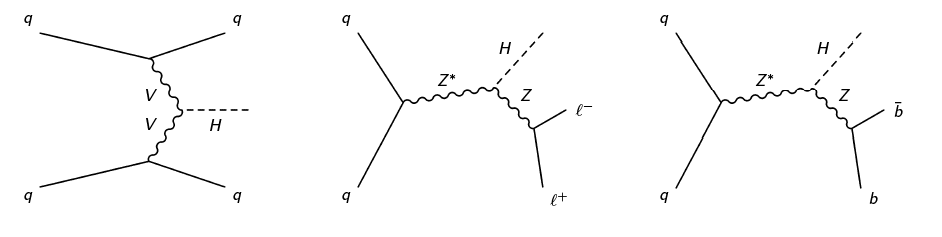
\includegraphics[width=\textwidth]{TalkPics/invcomb021213/feyndiags}
%% \begin{fmfgraph*}(100,70)
%%         \fmfleft{i1,i2}
%%         \fmfright{o1,o2,o3}
%%         \fmf{fermion}{i1,v1,o1}
%%         \fmf{fermion}{i2,v2,o3}
%%         \fmf{phantom,tension=4/5}{v1,v2}
%%         \fmffreeze
%%         \fmf{photon,label=$W,,Z$}{v1,v3}
%%         \fmf{photon,label=$W,,Z$}{v2,v3}
%%         \fmf{dashes}{v3,o2}
%%         \fmflabel{$q$}{i1}
%%         \fmflabel{$q$}{i2}
%%         \fmflabel{$q$}{o1}
%%         \fmflabel{$q$}{o3}
%%         \fmflabel{$H$}{o2}
%%       \end{fmfgraph*}
}
\date{}
\begin{document}
\begin{fmffile}{hig1330approvalfeynmandiags}

%TITLE PAGE
\section{Title}
\begin{frame}
  \titlepage
  
\end{frame}

%OUTLINE
\begin{frame}
  \frametitle{Overview}
  \begin{block}{}
    \scriptsize
    \begin{itemize}
    \item Fitted trigger efficiencies
    \item Look at some variants of the control plots
    \end{itemize}
  \end{block}
\end{frame}

\begin{frame}
  \frametitle{Trig Eff fit}
    \begin{block}{}
      \begin{itemize}
      \item Had problems with jumps in control plots
      \item[-] Jumps occured at trigger efficiency bin boundaries
      \item[-] Have fit error function to trigger turn on curves to try to solve problem
      \end{itemize}
    \end{block}
\end{frame}

%!!PUT SOME CONTROL PLOTS HERE
\begin{frame}
  \frametitle{L1 MET turn on}
  \begin{columns}
    \column{.5\textwidth}
    \begin{block}{L1 MET - full range}
      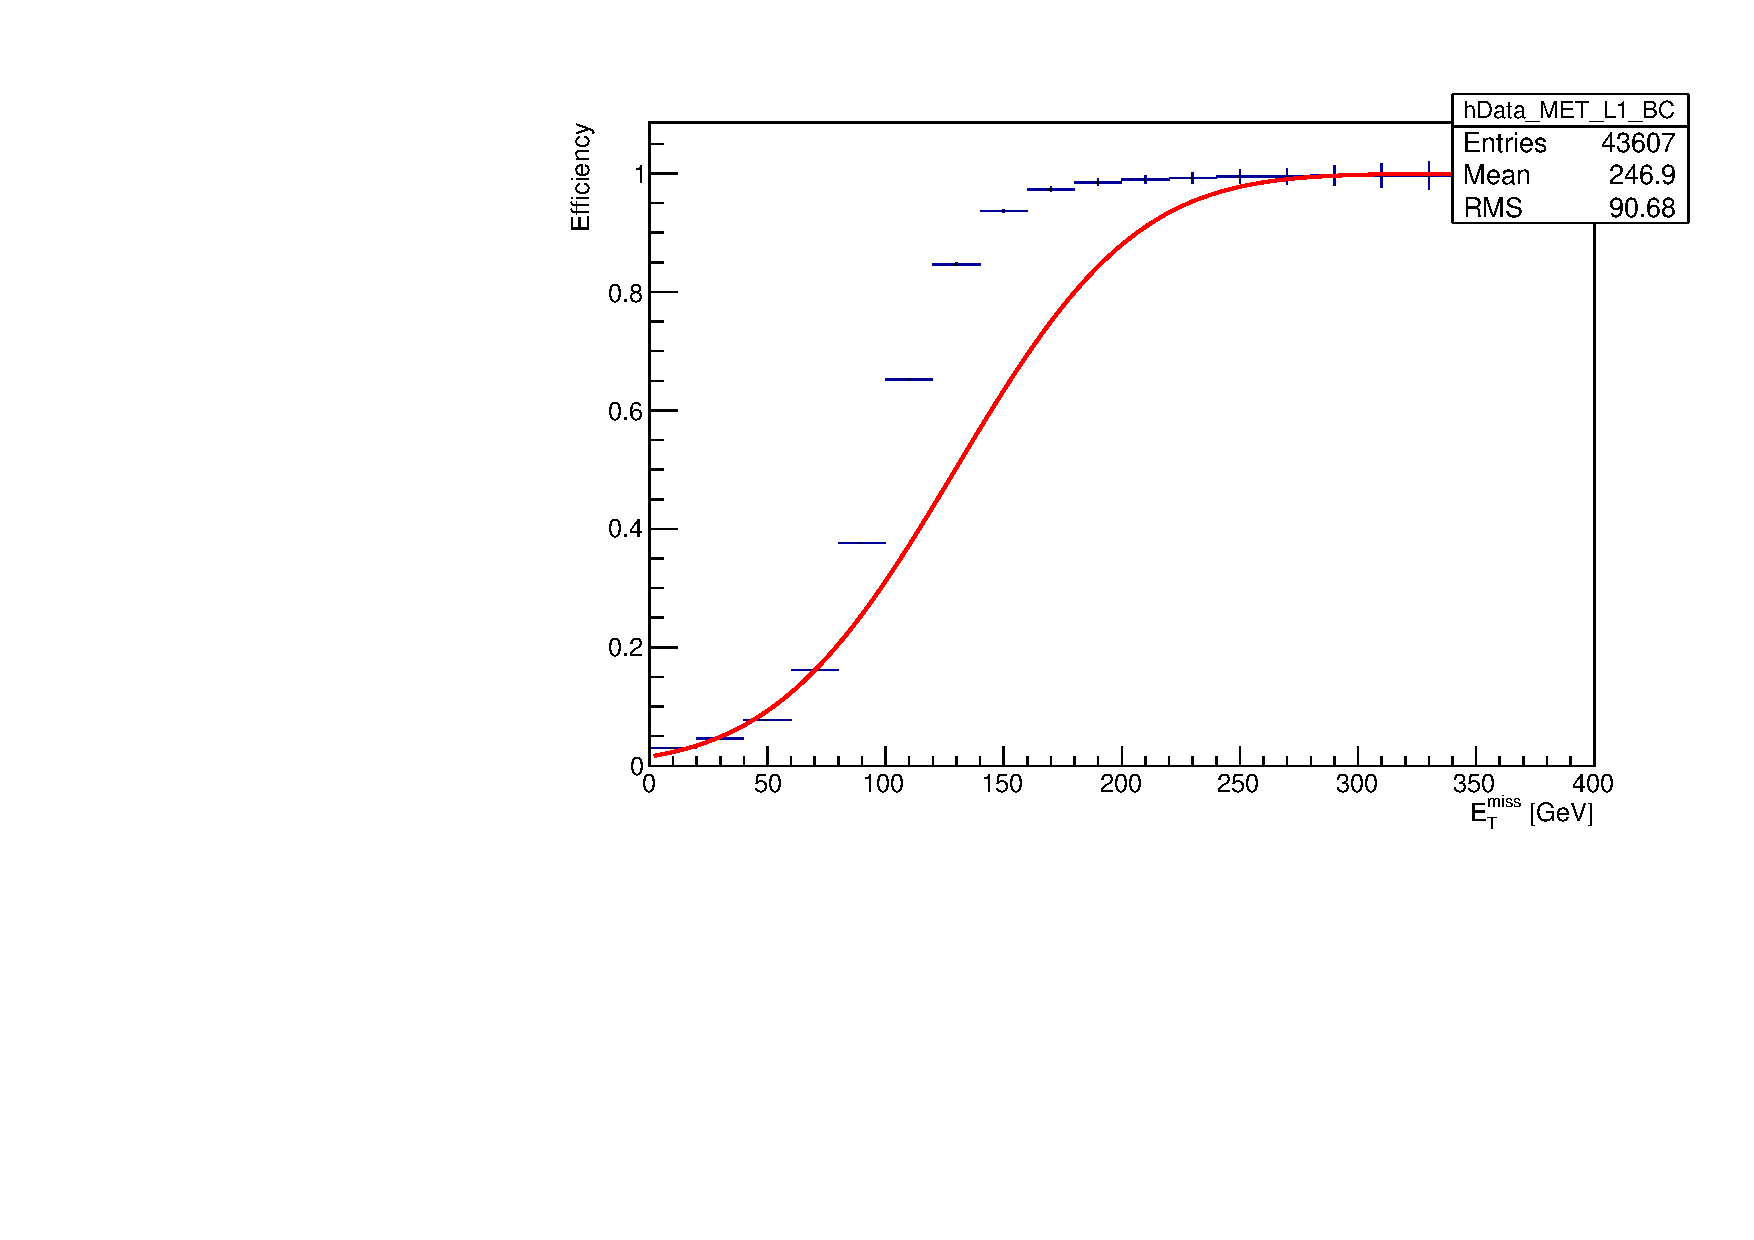
\includegraphics[width=\textwidth]{TalkPics/trigeffprog120814/0starthData_MET_L1_BC.pdf}
    \end{block}
    \column{.5\textwidth}
    \begin{block}{L1 MET - above 60}
      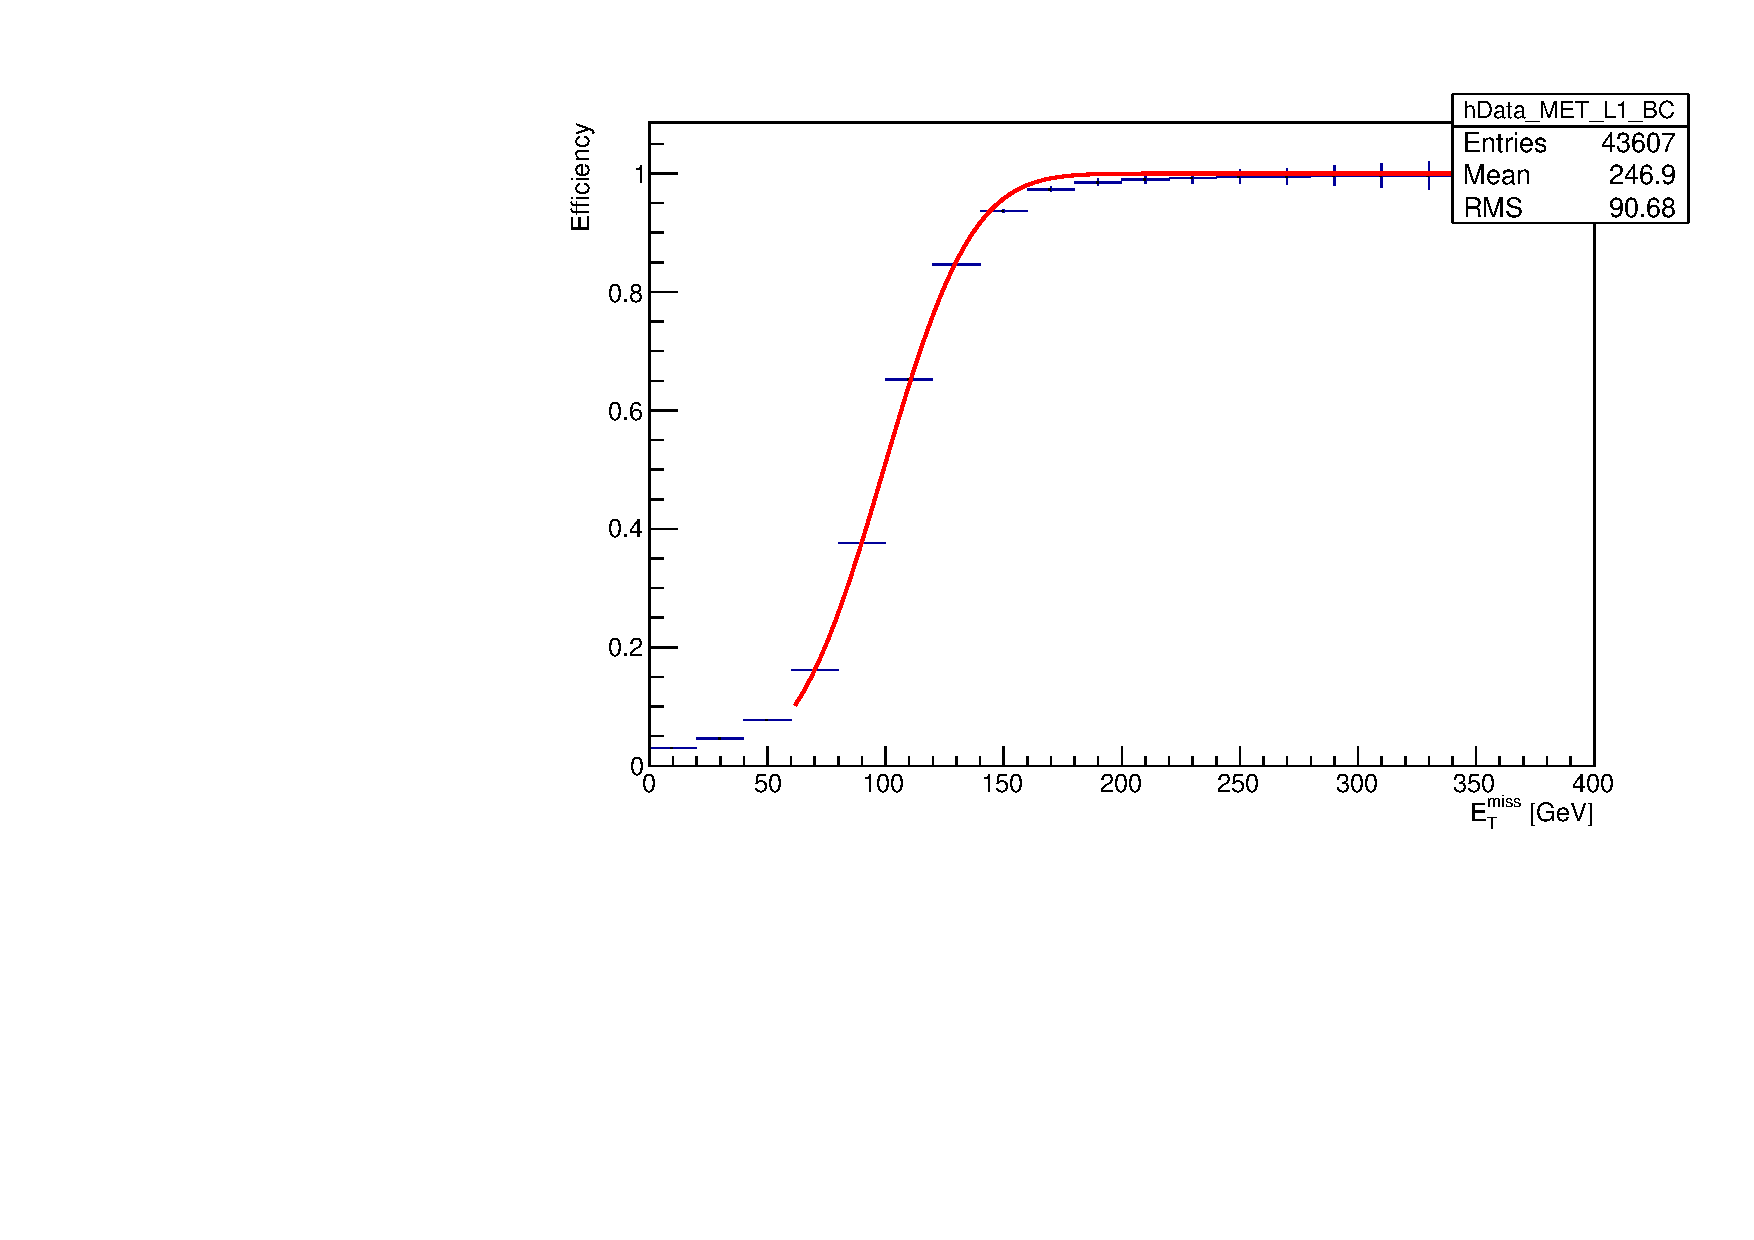
\includegraphics[width=\textwidth]{TalkPics/trigeffprog120814/hData_MET_L1_BC.pdf}
    \end{block}

  \end{columns}
\end{frame}

\begin{frame}
  \frametitle{L1 MET turn on}
  \begin{columns}
    \column{.5\textwidth}
    \begin{block}{L1 MET - A}
      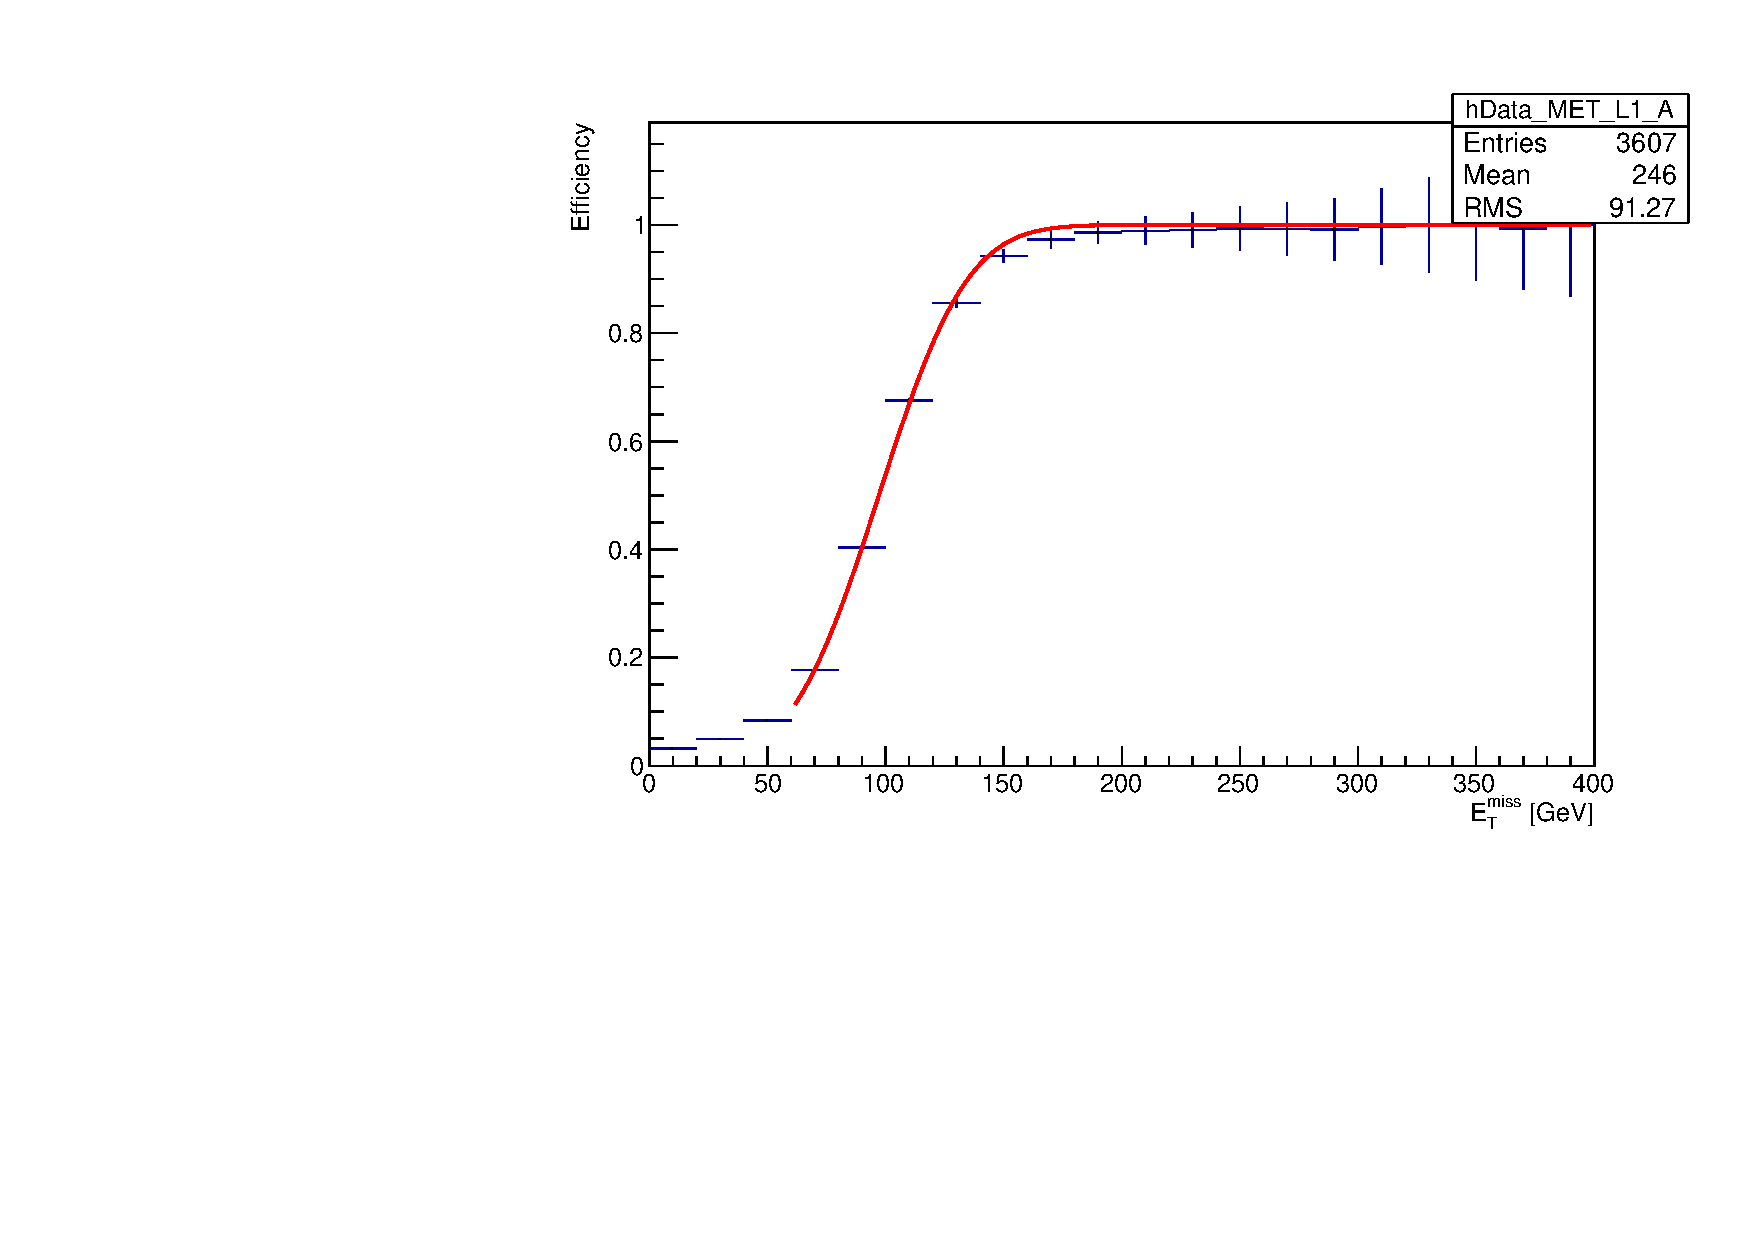
\includegraphics[width=\textwidth]{TalkPics/trigeffprog120814/hData_MET_L1_A.pdf}
    \end{block}
    \column{.5\textwidth}
    \begin{block}{L1 MET - BC}
      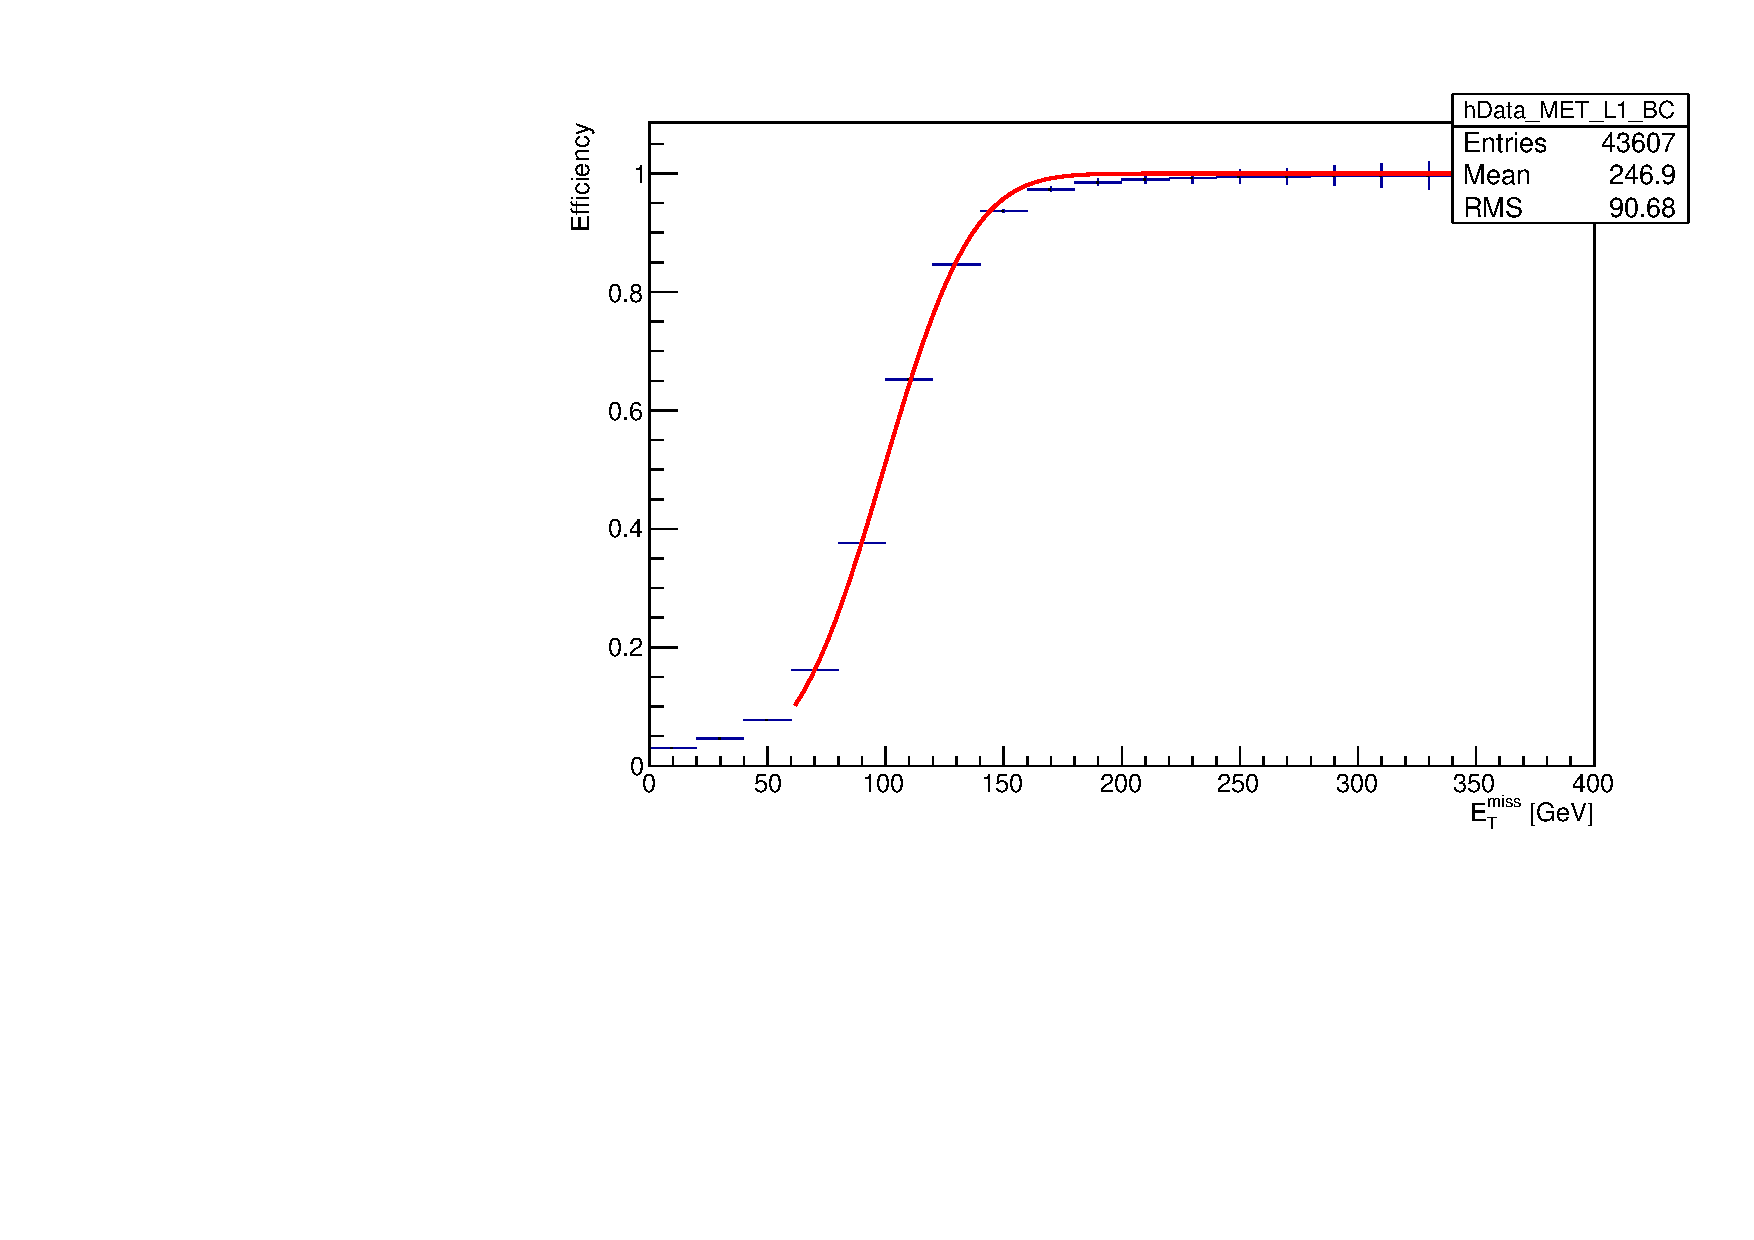
\includegraphics[width=\textwidth]{TalkPics/trigeffprog120814/hData_MET_L1_BC.pdf}
    \end{block}

  \end{columns}
\end{frame}

\begin{frame}
  \frametitle{L1 MET turn on}
  \begin{columns}
    \column{.5\textwidth}
    \begin{block}{L1 MET - D}
      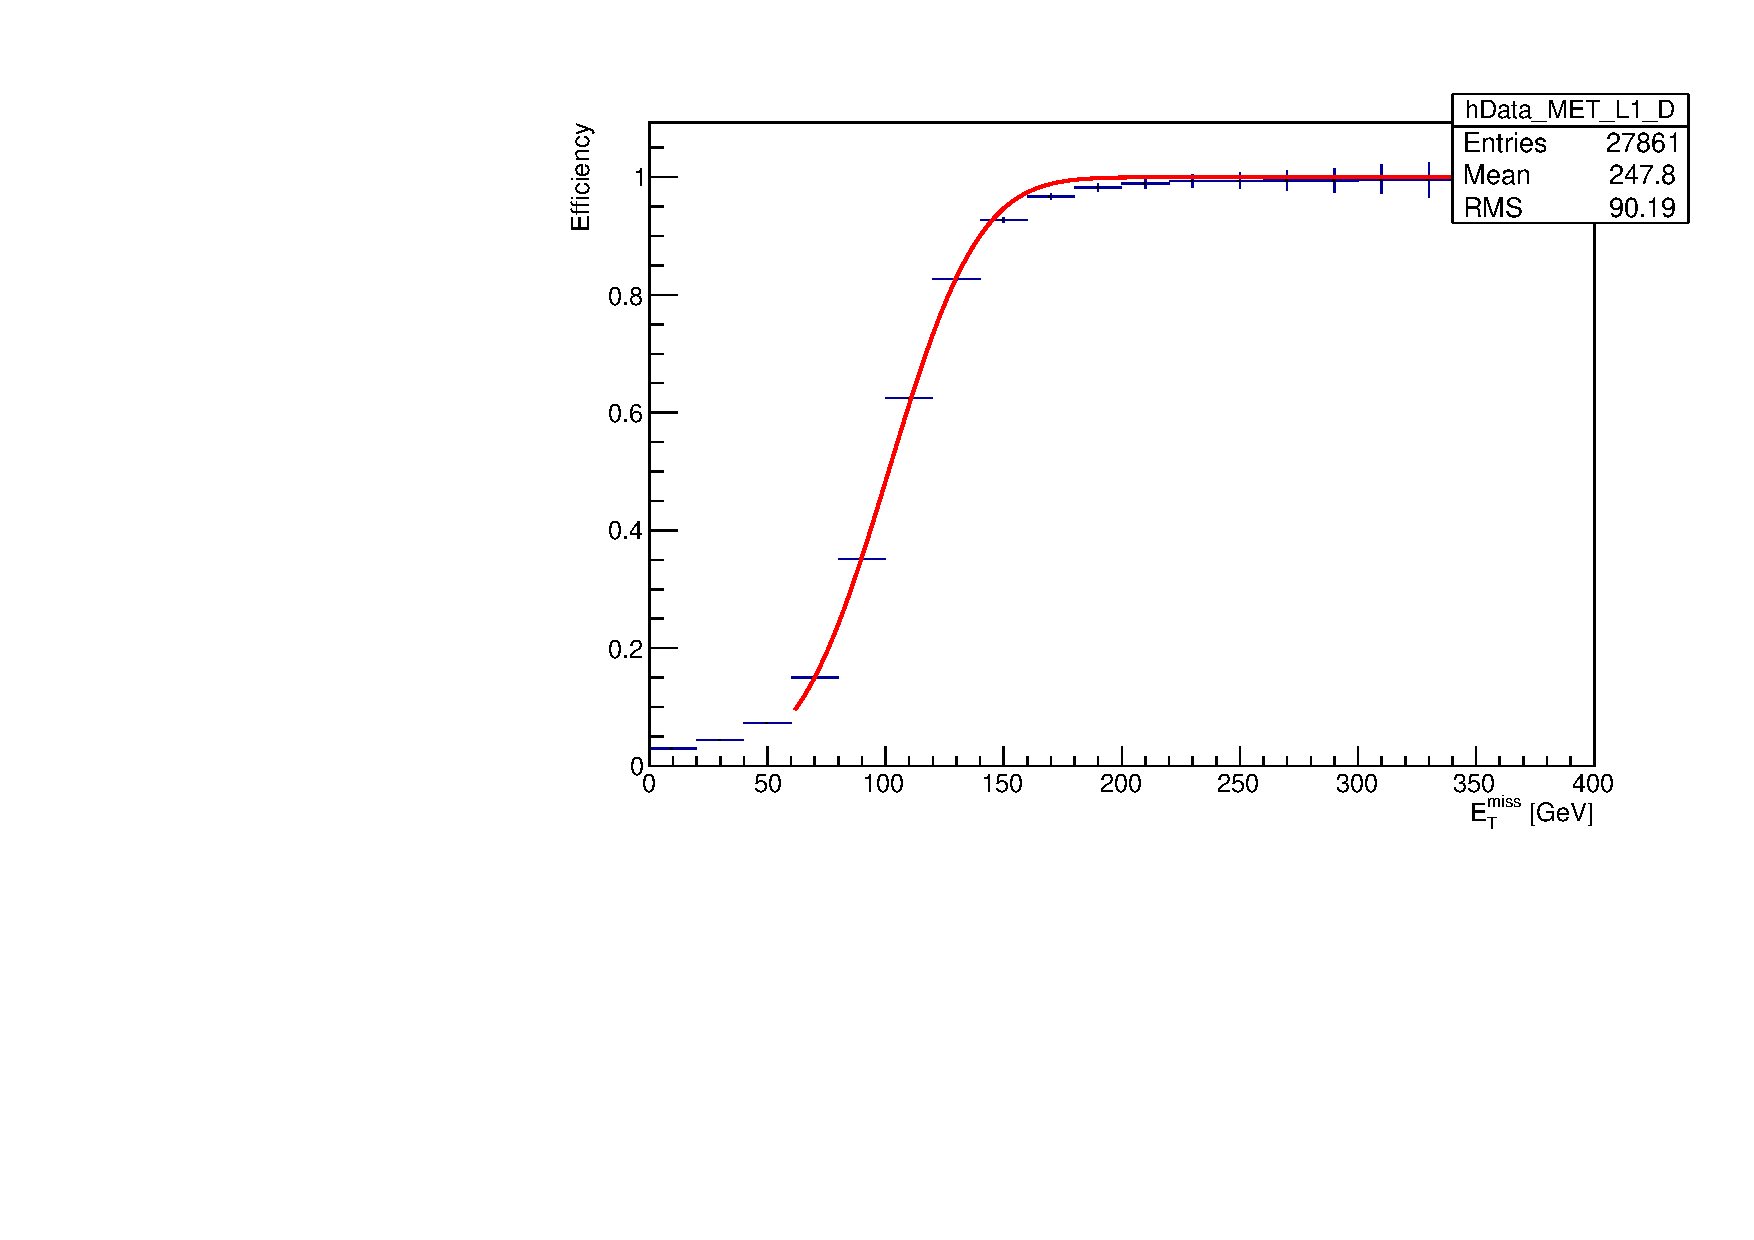
\includegraphics[width=\textwidth]{TalkPics/trigeffprog120814/hData_MET_L1_D.pdf}
    \end{block}
    \column{.5\textwidth}

  \end{columns}
\end{frame}

\begin{frame}
  \frametitle{HLT MET turn on}
  \begin{columns}
    \column{.5\textwidth}
    \begin{block}{HLT MET - A}
      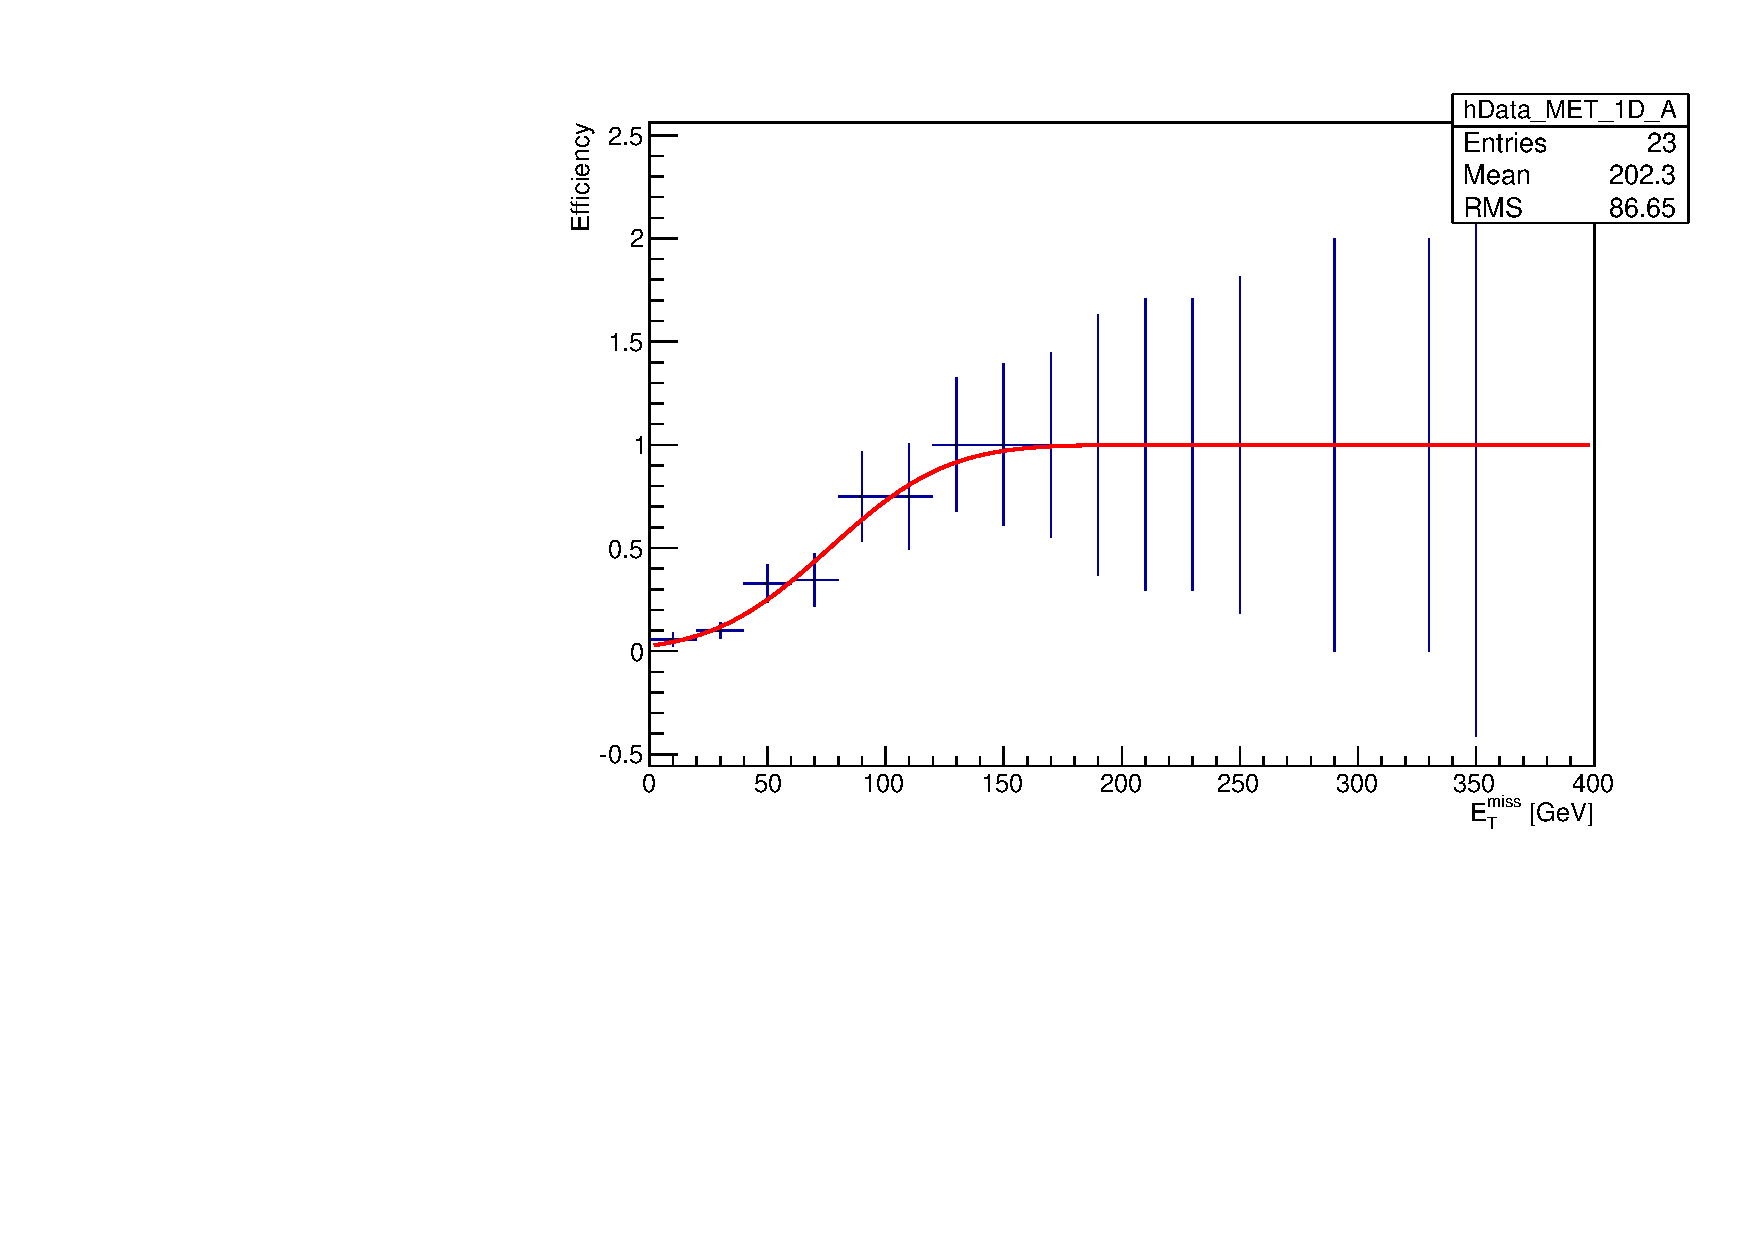
\includegraphics[width=\textwidth]{TalkPics/trigeffprog120814/hData_MET_1D_A.pdf}
    \end{block}
    \column{.5\textwidth}
    \begin{block}{HLT MET - BC}
      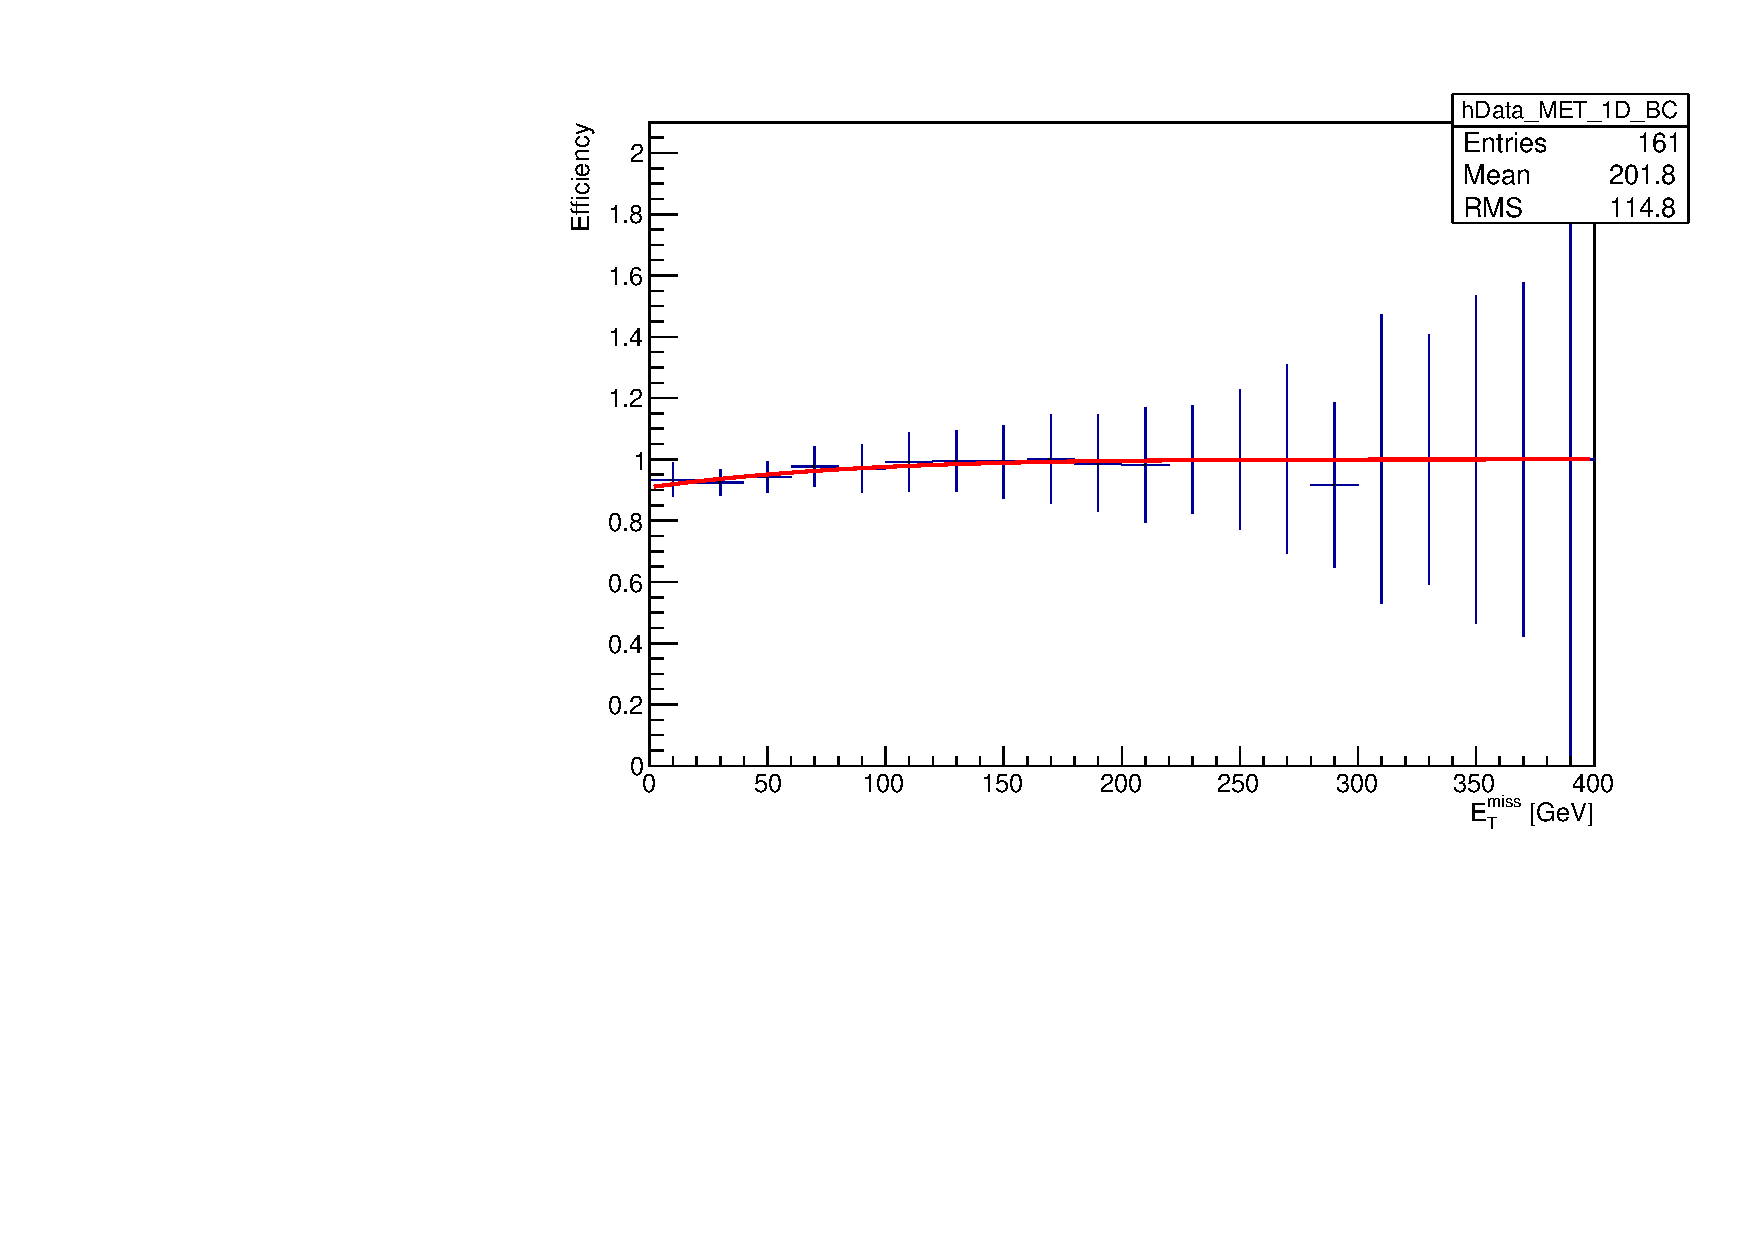
\includegraphics[width=\textwidth]{TalkPics/trigeffprog120814/hData_MET_1D_BC.pdf}
    \end{block}

  \end{columns}
\end{frame}

\begin{frame}
  \frametitle{HLT MET turn on}
  \begin{columns}
    \column{.5\textwidth}
    \begin{block}{HLT MET - D}
      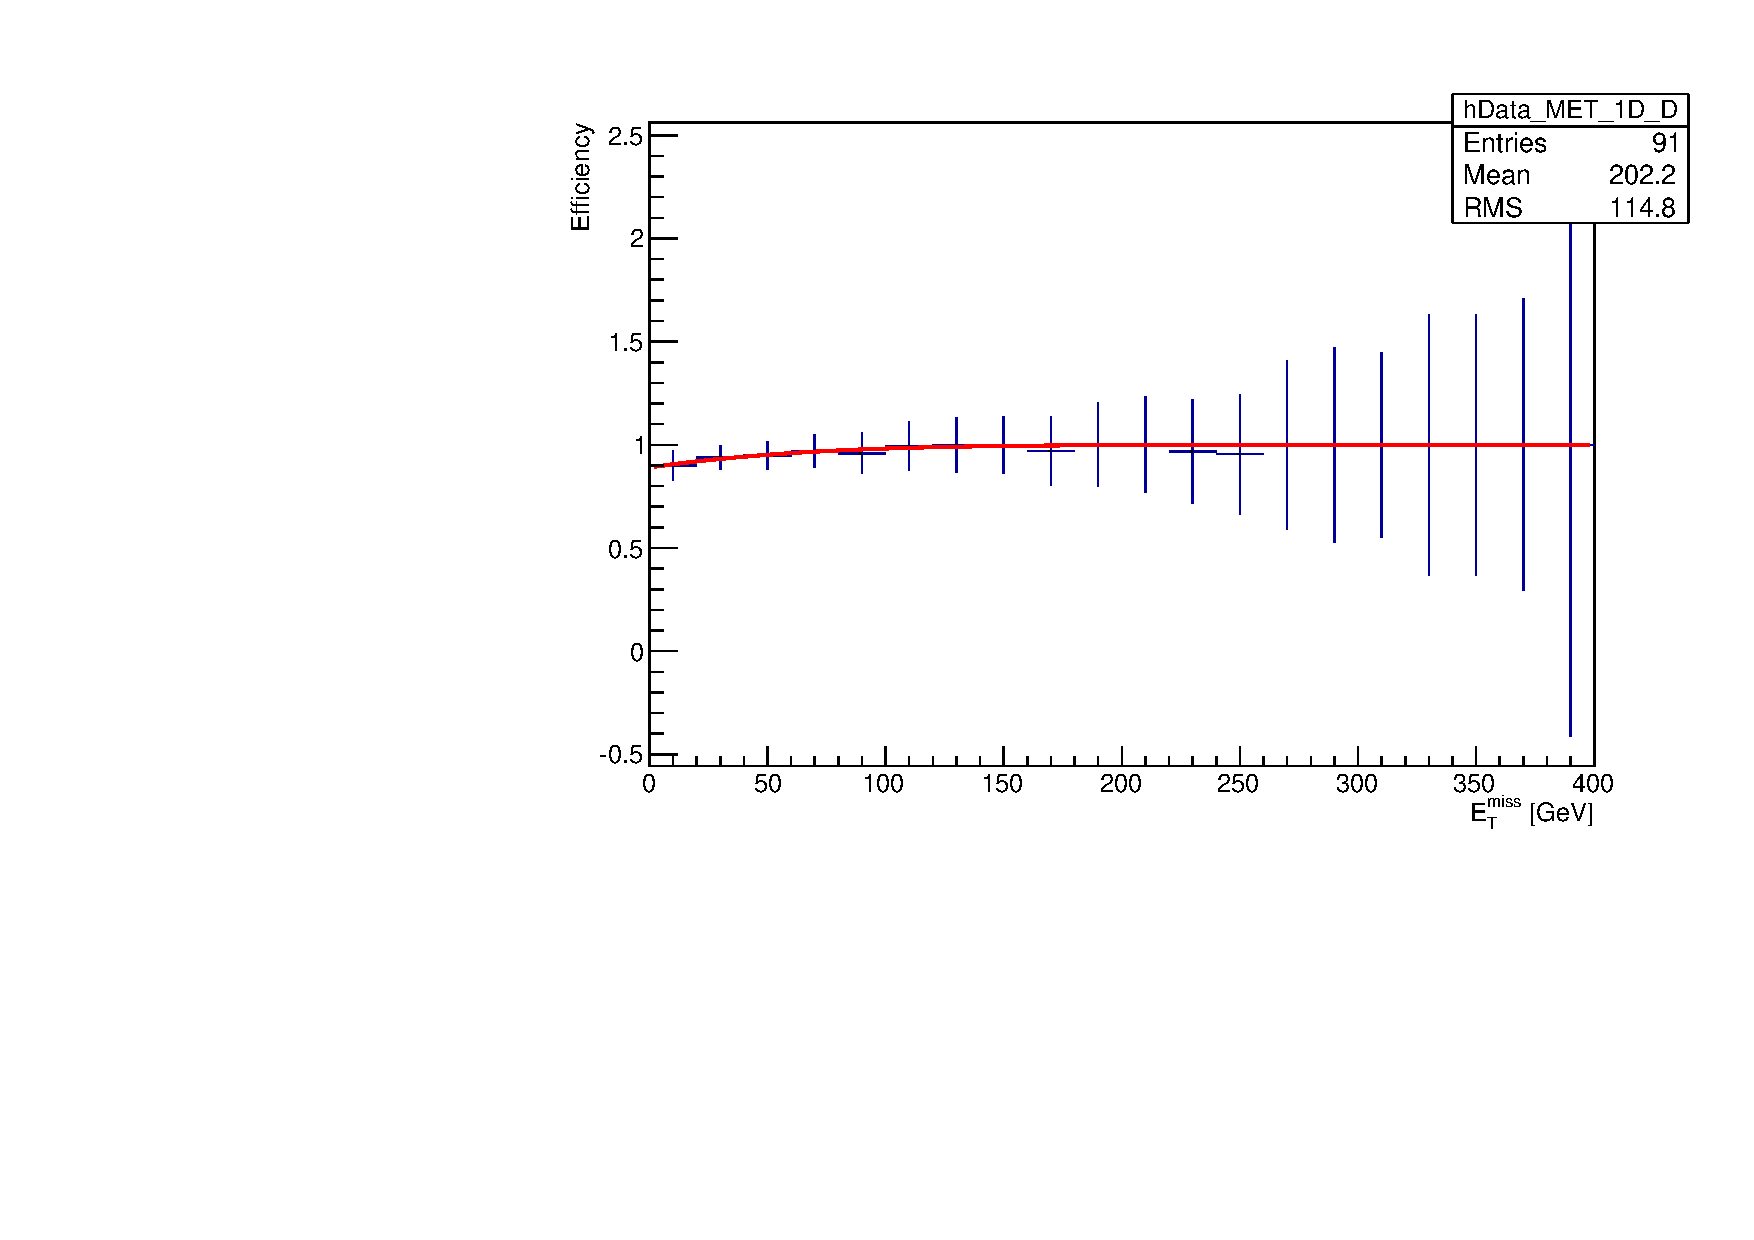
\includegraphics[width=\textwidth]{TalkPics/trigeffprog120814/hData_MET_1D_D.pdf}
    \end{block}
    \column{.5\textwidth}

  \end{columns}
\end{frame}

\begin{frame}
  \frametitle{HLT MJJ turn on}
  \begin{columns}
    \column{.5\textwidth}
    \begin{block}{HLT MJJ - A}
      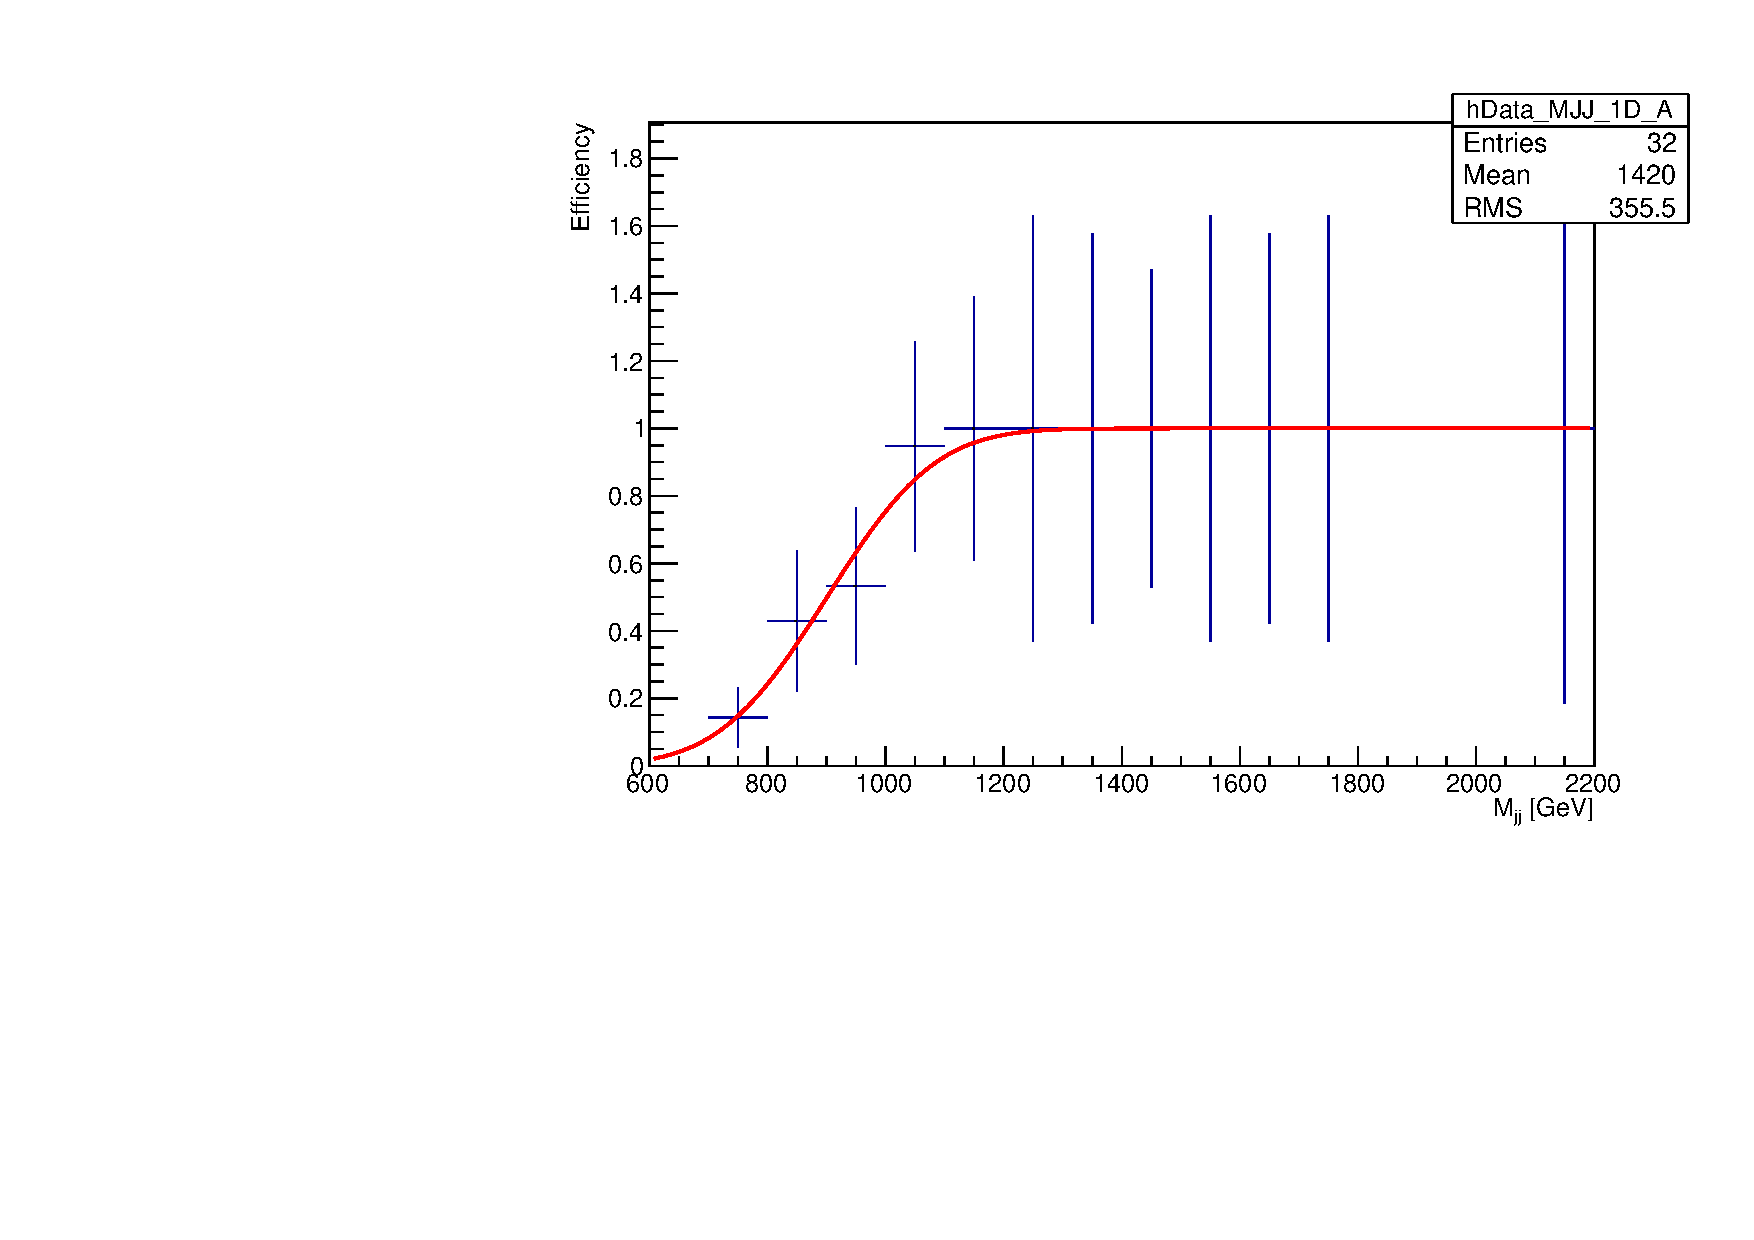
\includegraphics[width=\textwidth]{TalkPics/trigeffprog120814/hData_MJJ_1D_A.pdf}
    \end{block}
    \column{.5\textwidth}
    \begin{block}{HLT MJJ - BC}
      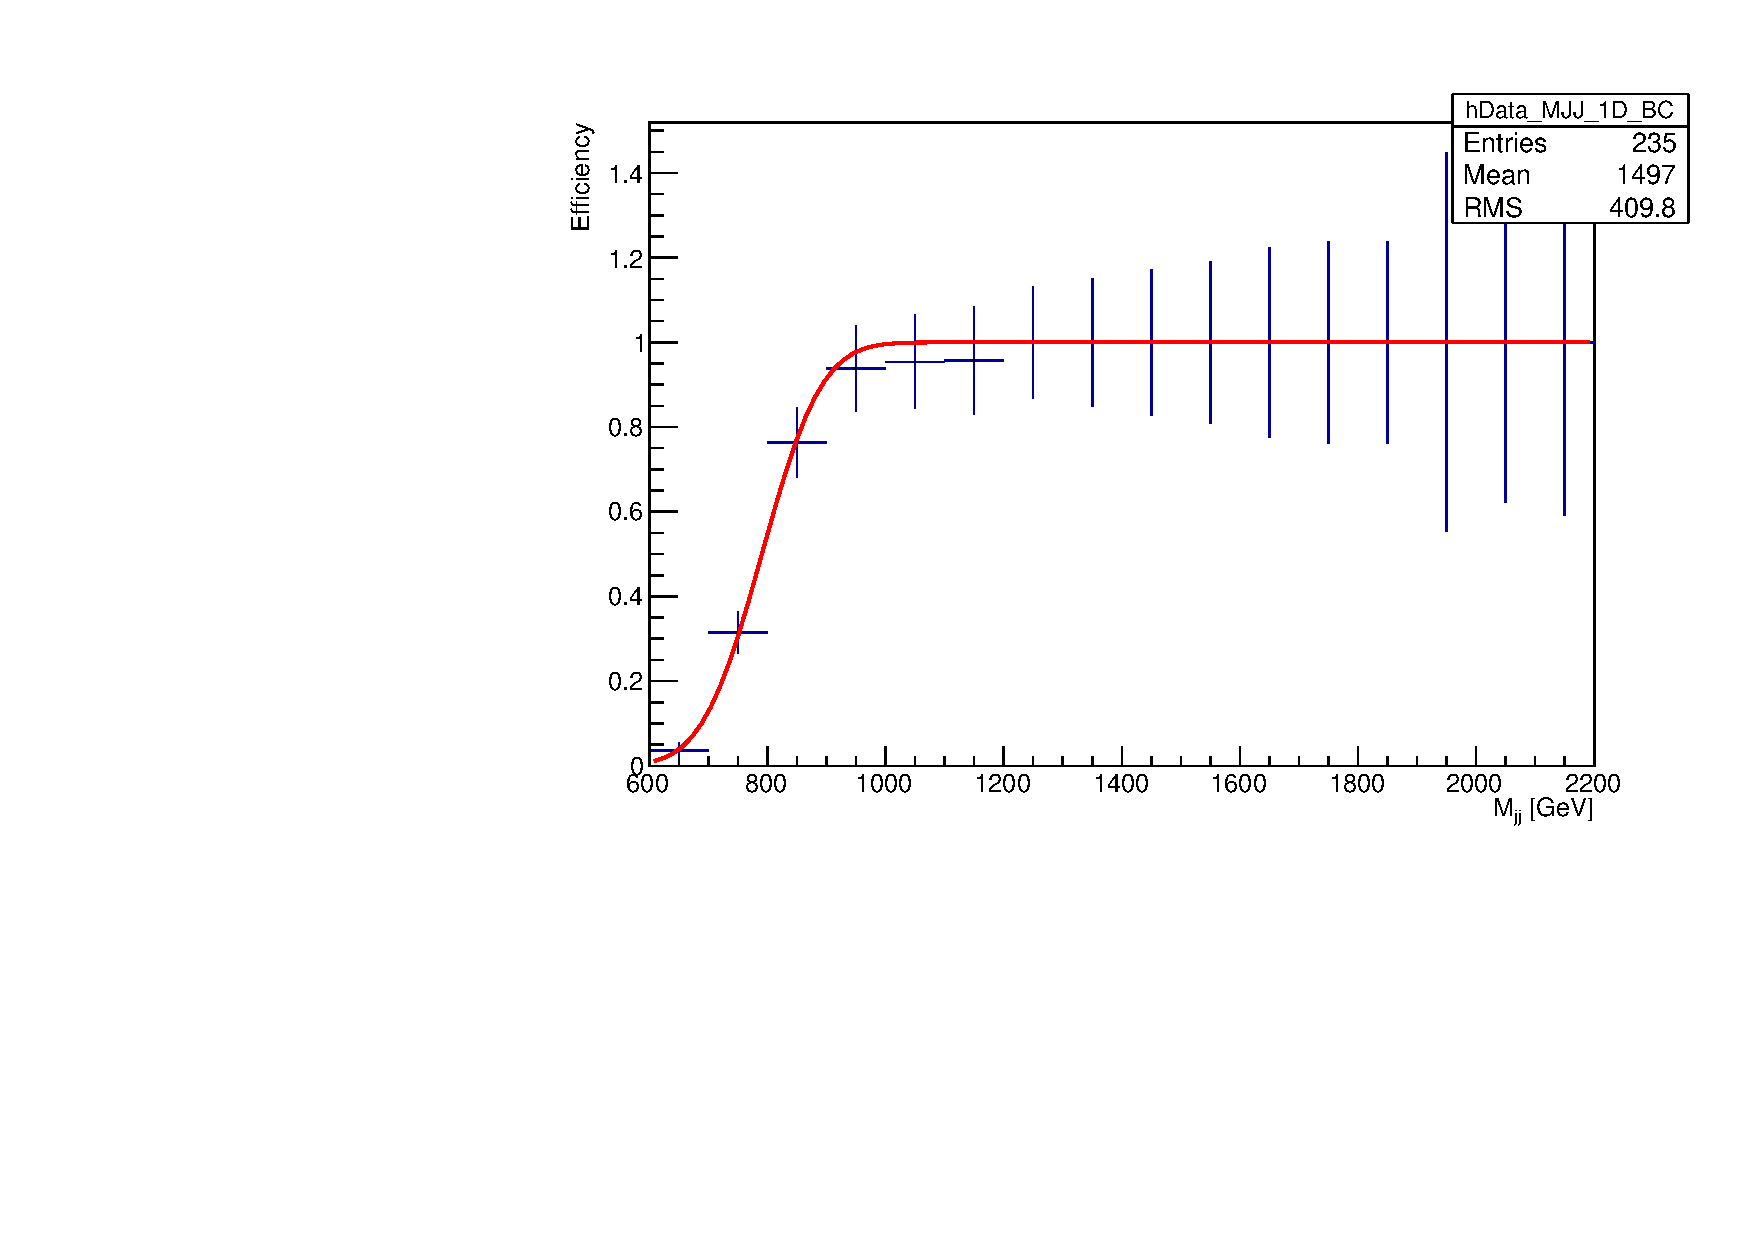
\includegraphics[width=\textwidth]{TalkPics/trigeffprog120814/hData_MJJ_1D_BC.pdf}
    \end{block}

  \end{columns}
\end{frame}

\begin{frame}
  \frametitle{HLT MJJ turn on}
  \begin{columns}
    \column{.5\textwidth}
    \begin{block}{HLT MJJ - D}
      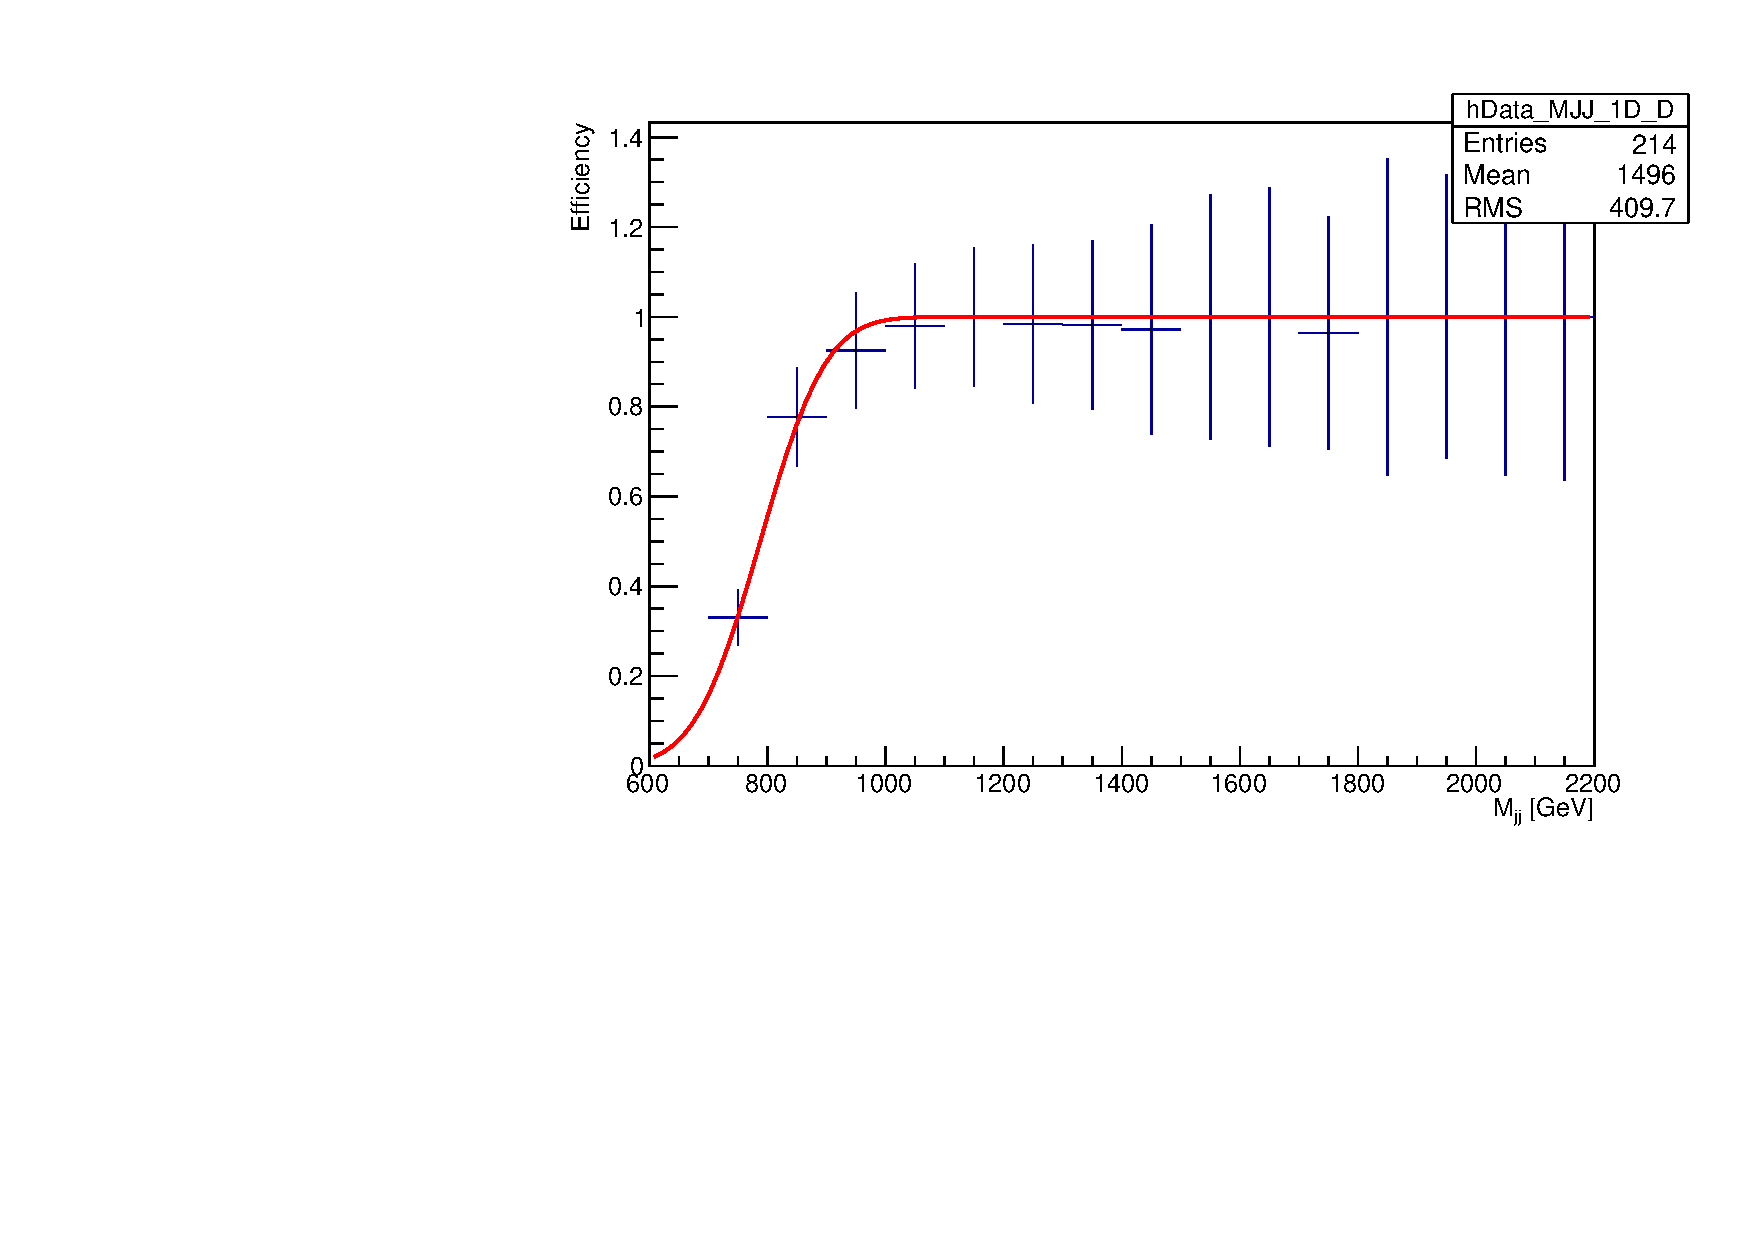
\includegraphics[width=\textwidth]{TalkPics/trigeffprog120814/hData_MJJ_1D_D.pdf}
    \end{block}
    \column{.5\textwidth}

  \end{columns}
\end{frame}

\begin{frame}
  \frametitle{HLT JET2 turn on}
  \begin{columns}
    \column{.5\textwidth}
    \begin{block}{HLT JET2 - A}
      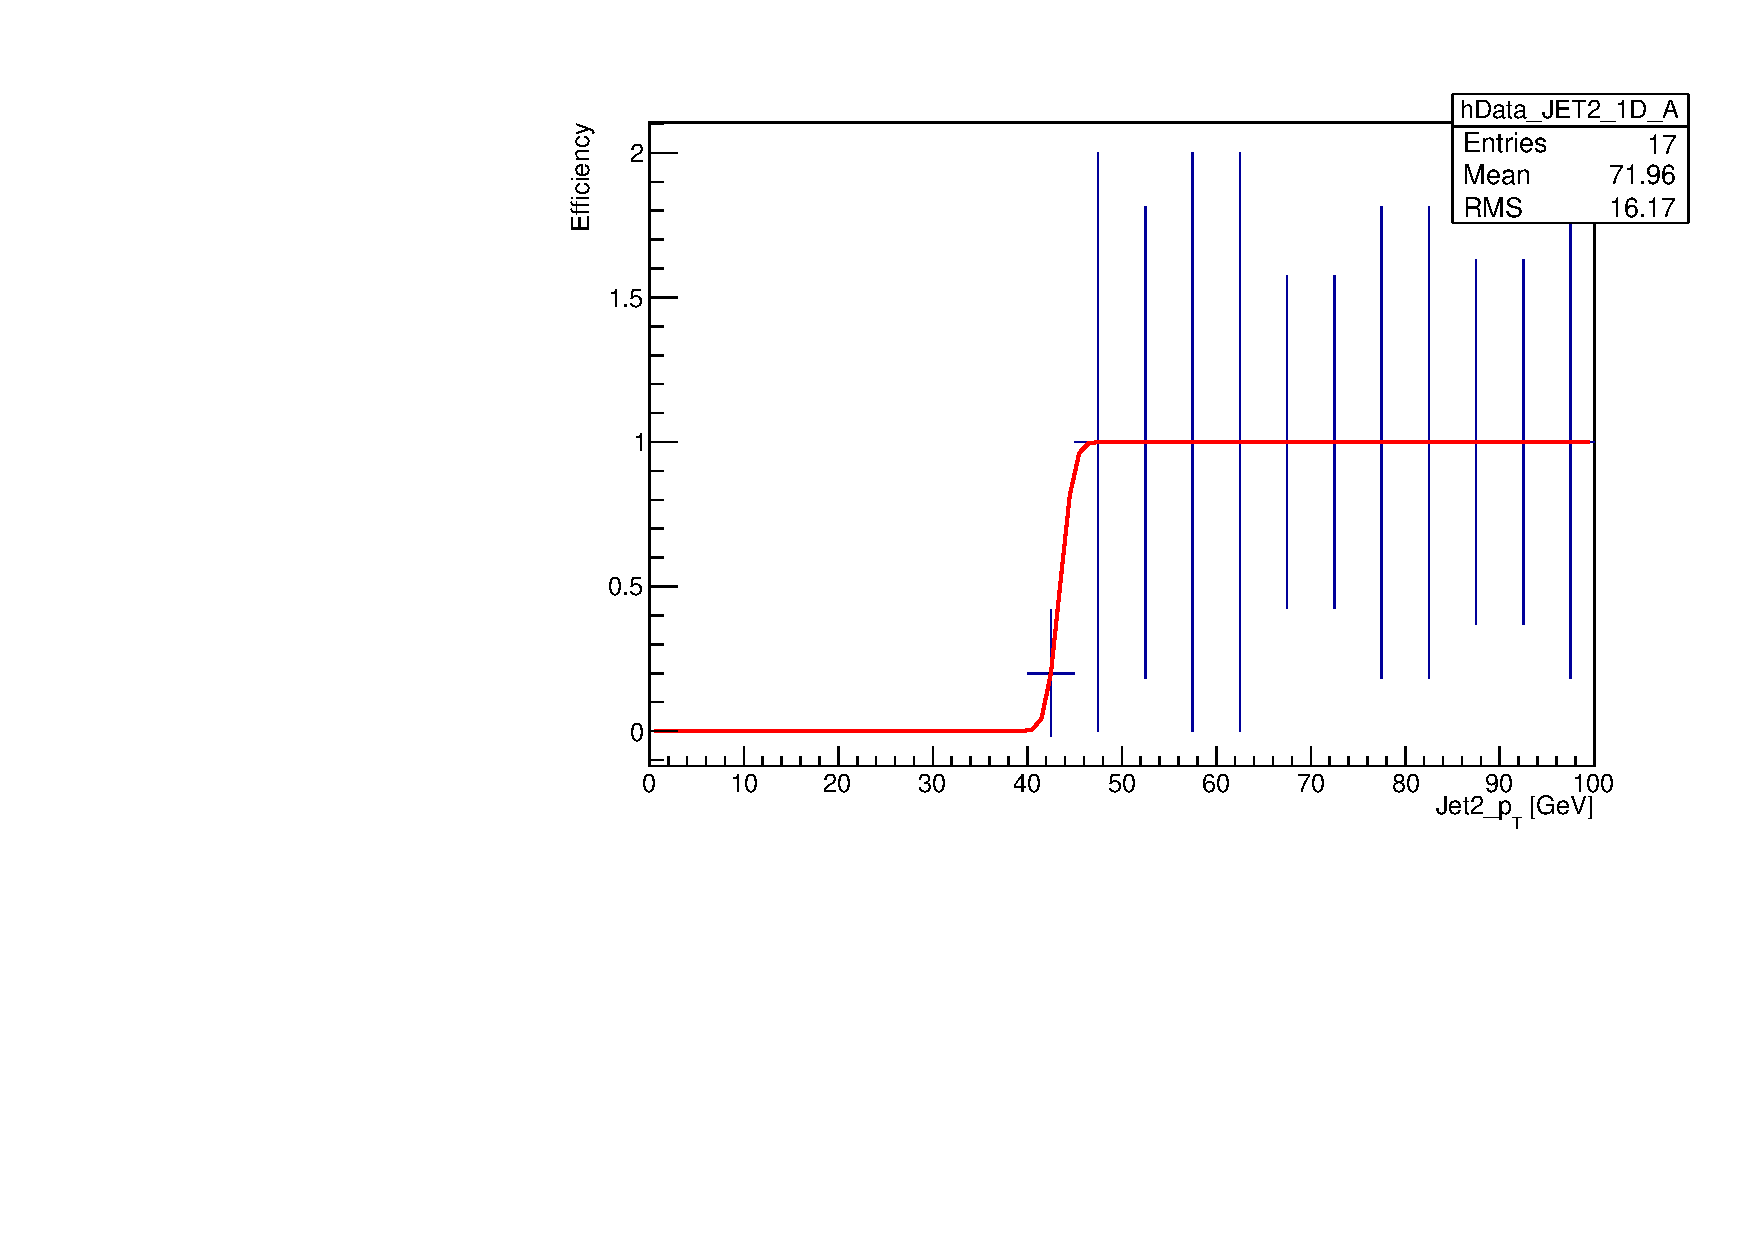
\includegraphics[width=\textwidth]{TalkPics/trigeffprog120814/hData_JET2_1D_A.pdf}
    \end{block}
    \column{.5\textwidth}
    \begin{block}{HLT JET2 - BC}
      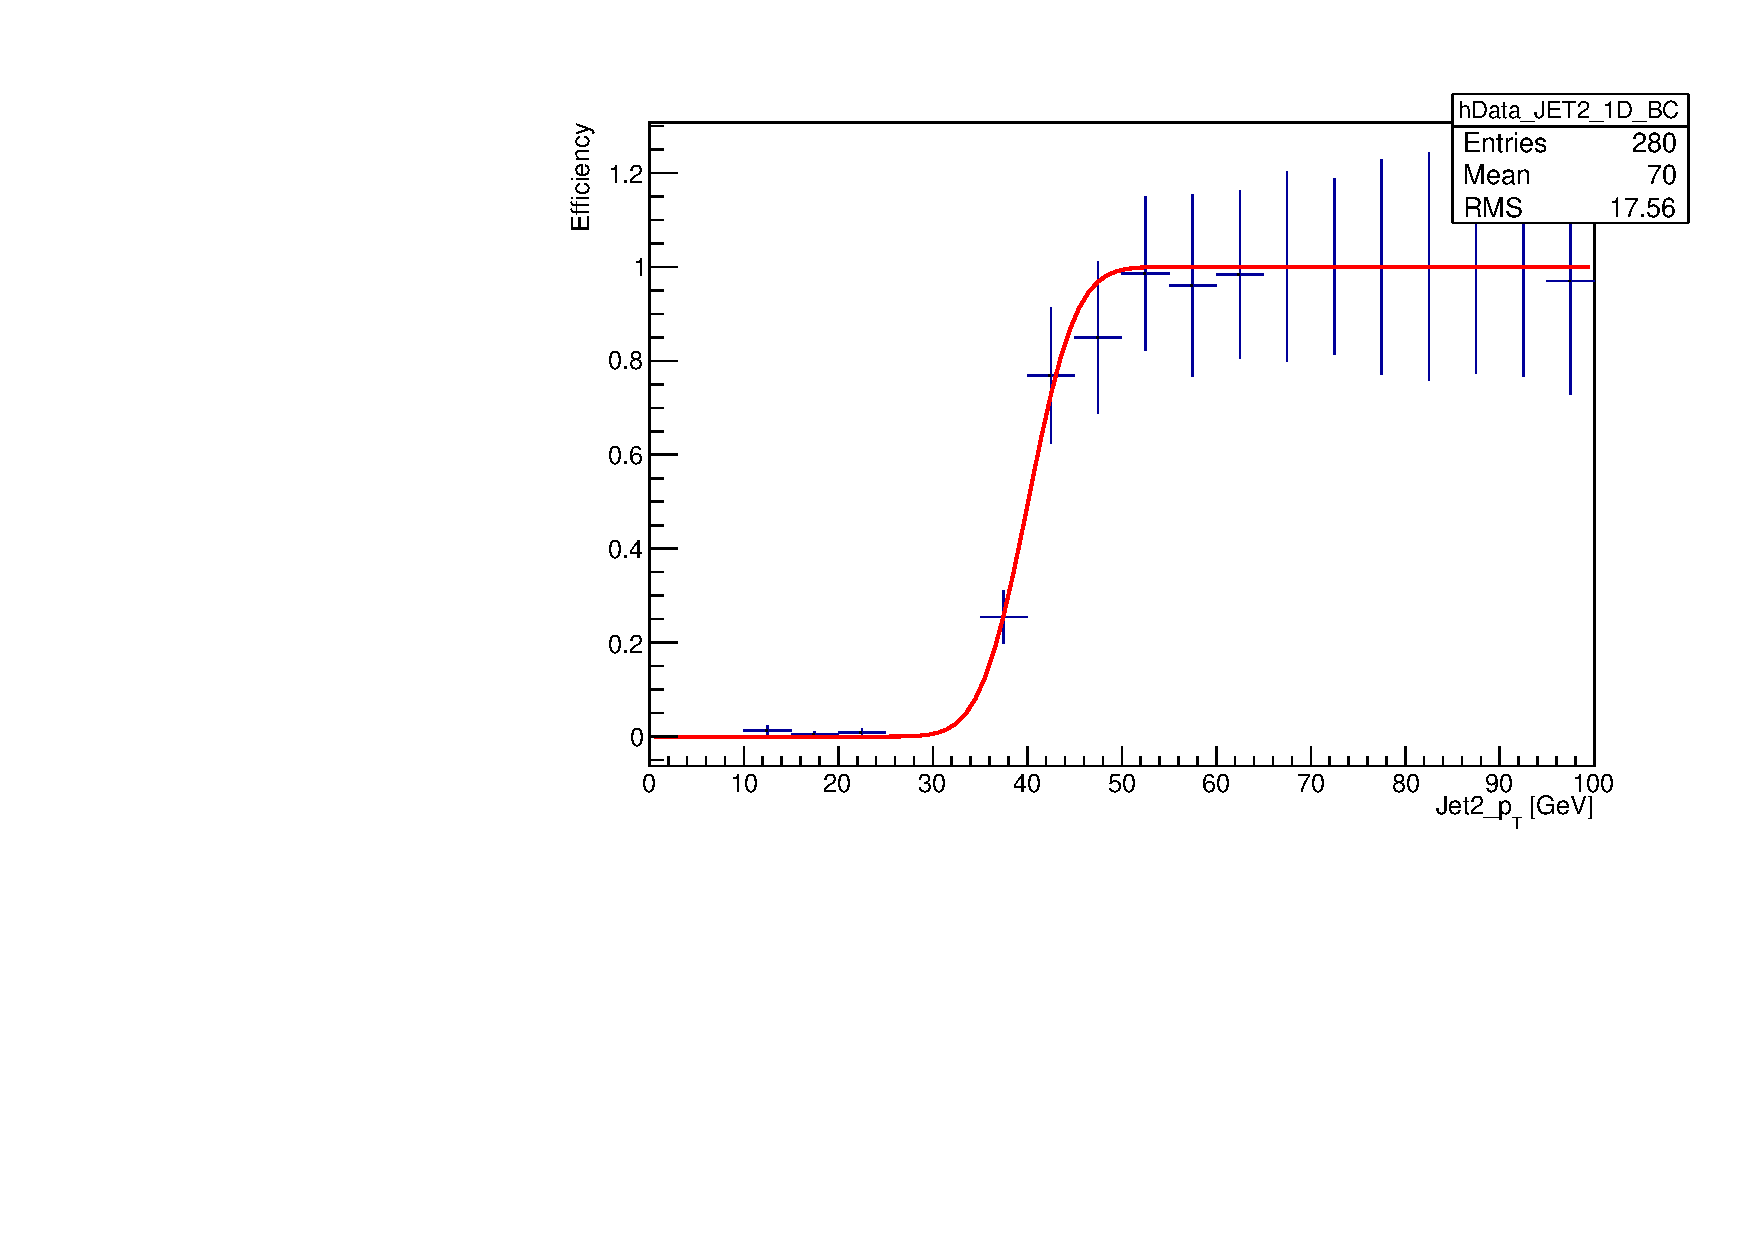
\includegraphics[width=\textwidth]{TalkPics/trigeffprog120814/hData_JET2_1D_BC.pdf}
    \end{block}

  \end{columns}
\end{frame}

\begin{frame}
  \frametitle{HLT JET2 turn on}
  \begin{columns}
    \column{.5\textwidth}
    \begin{block}{HLT JET2 - D}
      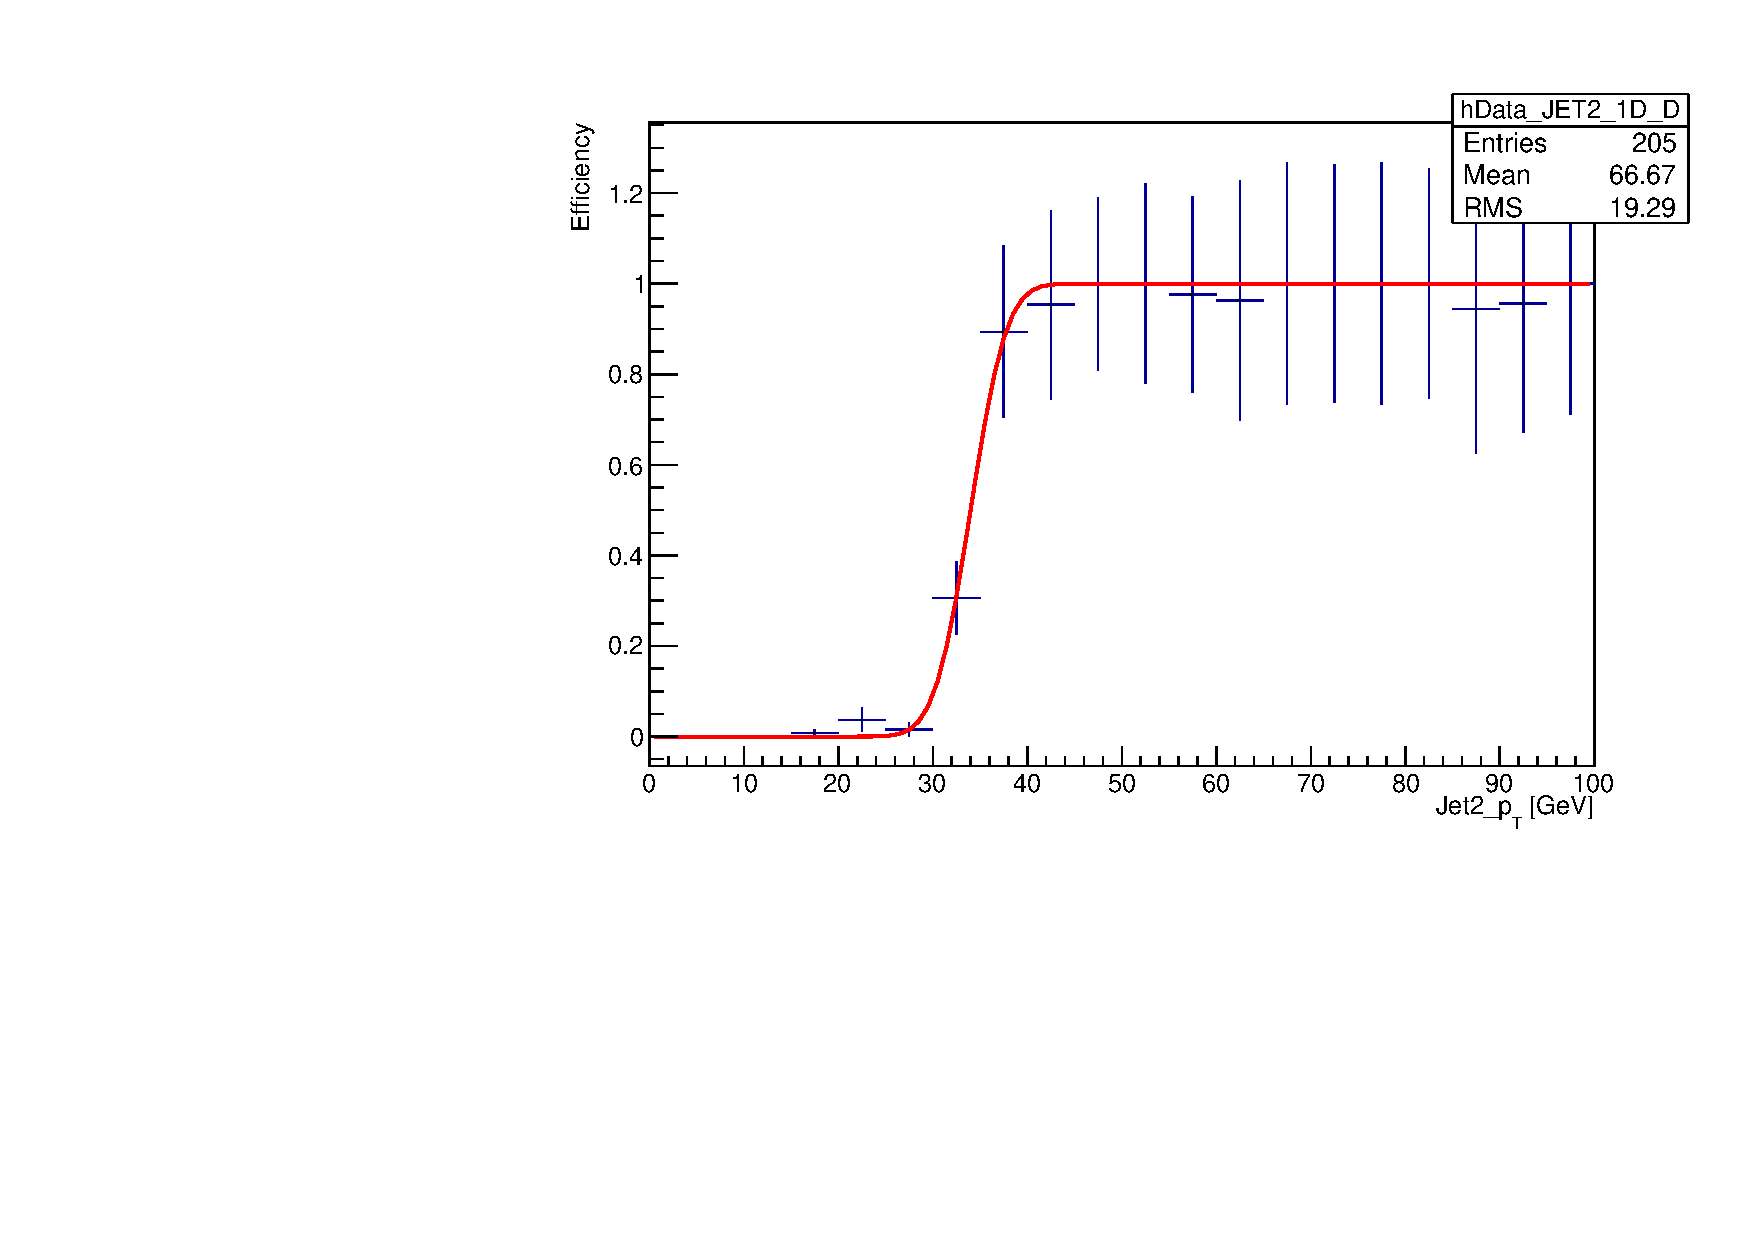
\includegraphics[width=\textwidth]{TalkPics/trigeffprog120814/hData_JET2_1D_D.pdf}
    \end{block}
    \column{.5\textwidth}

  \end{columns}
\end{frame}

\begin{frame}
  \frametitle{New Control Plots}
    \begin{block}{}
      \begin{itemize}
      \item Add met$>60$ cut because of trigger turn on fit
      \item Other cuts are: $jet1_pt>50,jet2_pt>50,dijet_deta>3.6,metnomu_significance>3,jetmetnomu_mindphi>1.5$
      \item Later plots also have: $!(metnomuons<130\&\&dijet_M<1100)$
      \end{itemize}
    \end{block}
\end{frame}

\begin{frame}
  \frametitle{New control plots}
  \begin{columns}
    \column{.5\textwidth}
    \begin{block}{Jet 1 pt}
      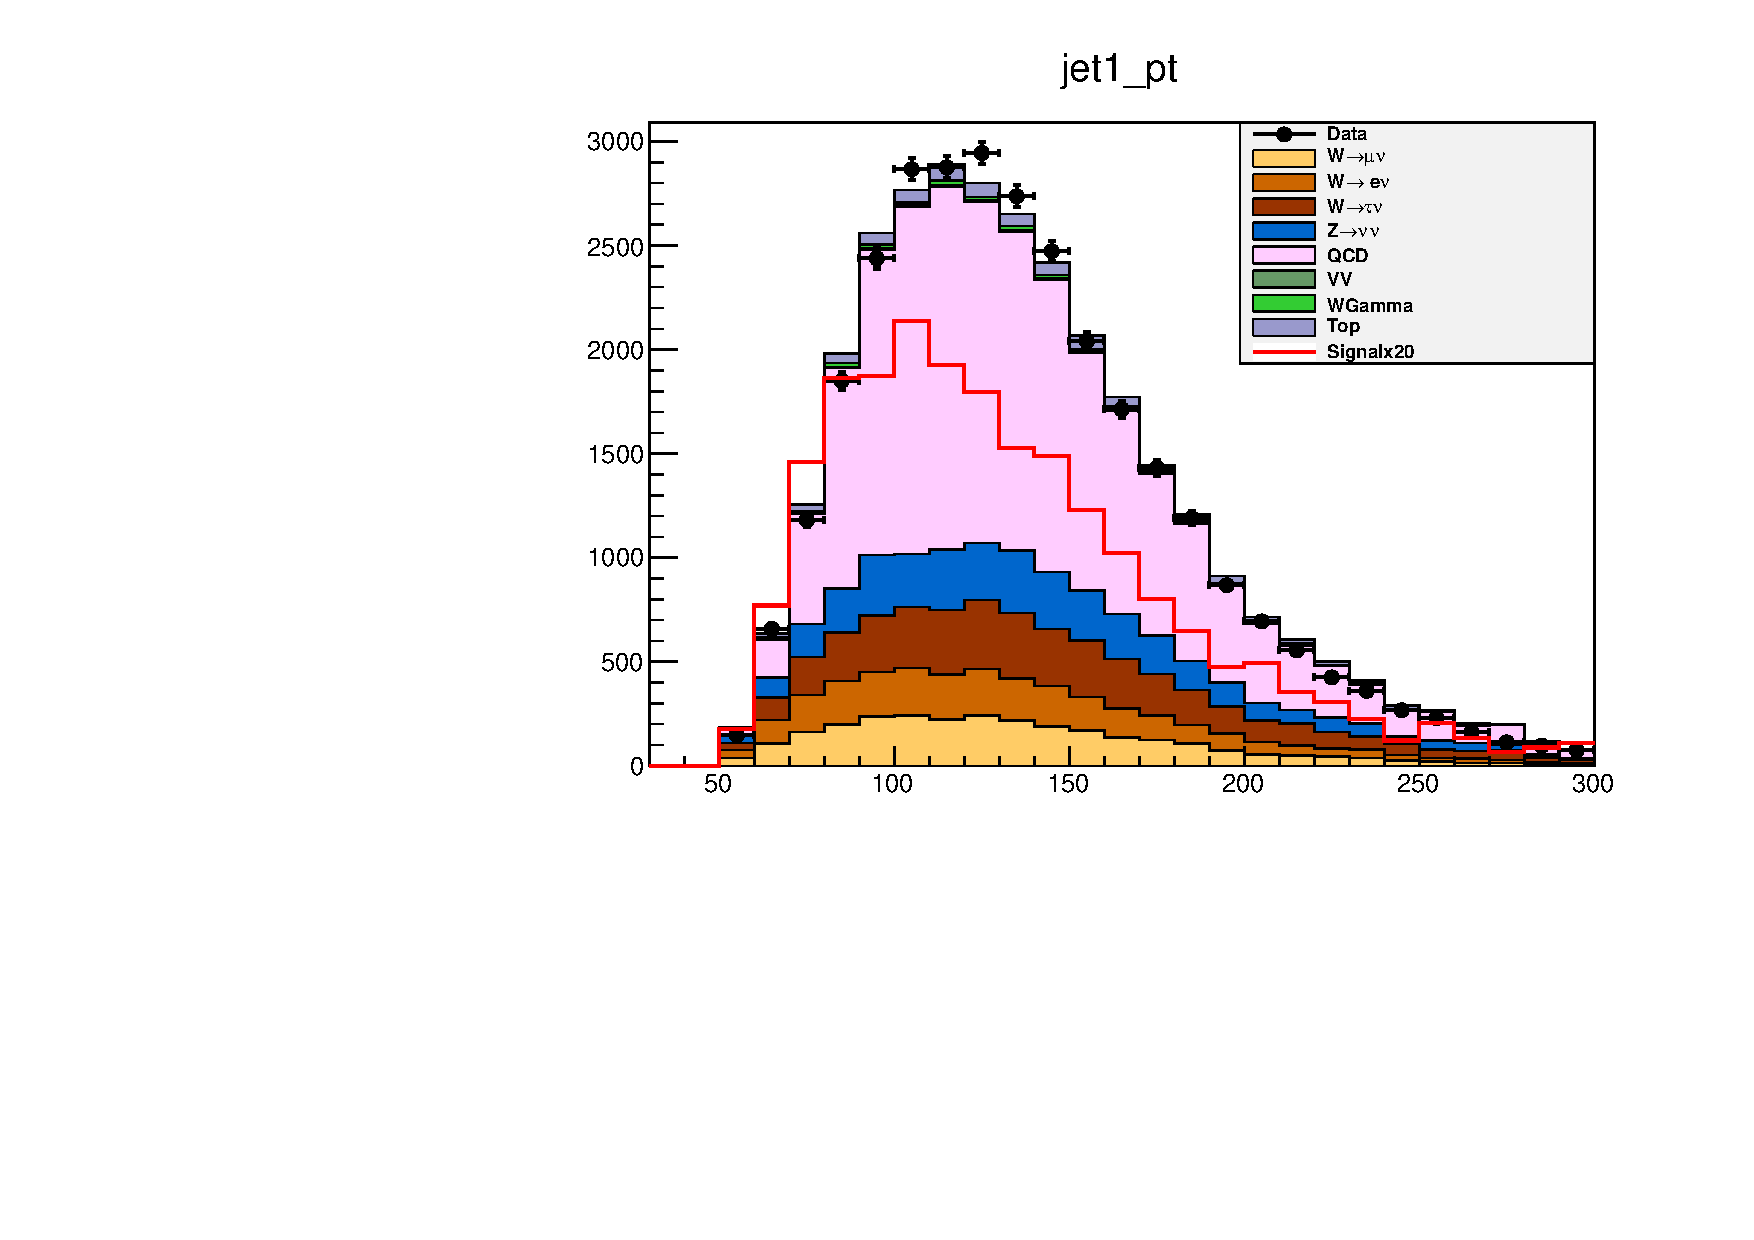
\includegraphics[width=\textwidth]{TalkPics/trigeffprog120814/nometmjjcutsig_jet1pt.pdf}
    \end{block}
    \column{.5\textwidth}
    \begin{block}{Jet 2 pt}
      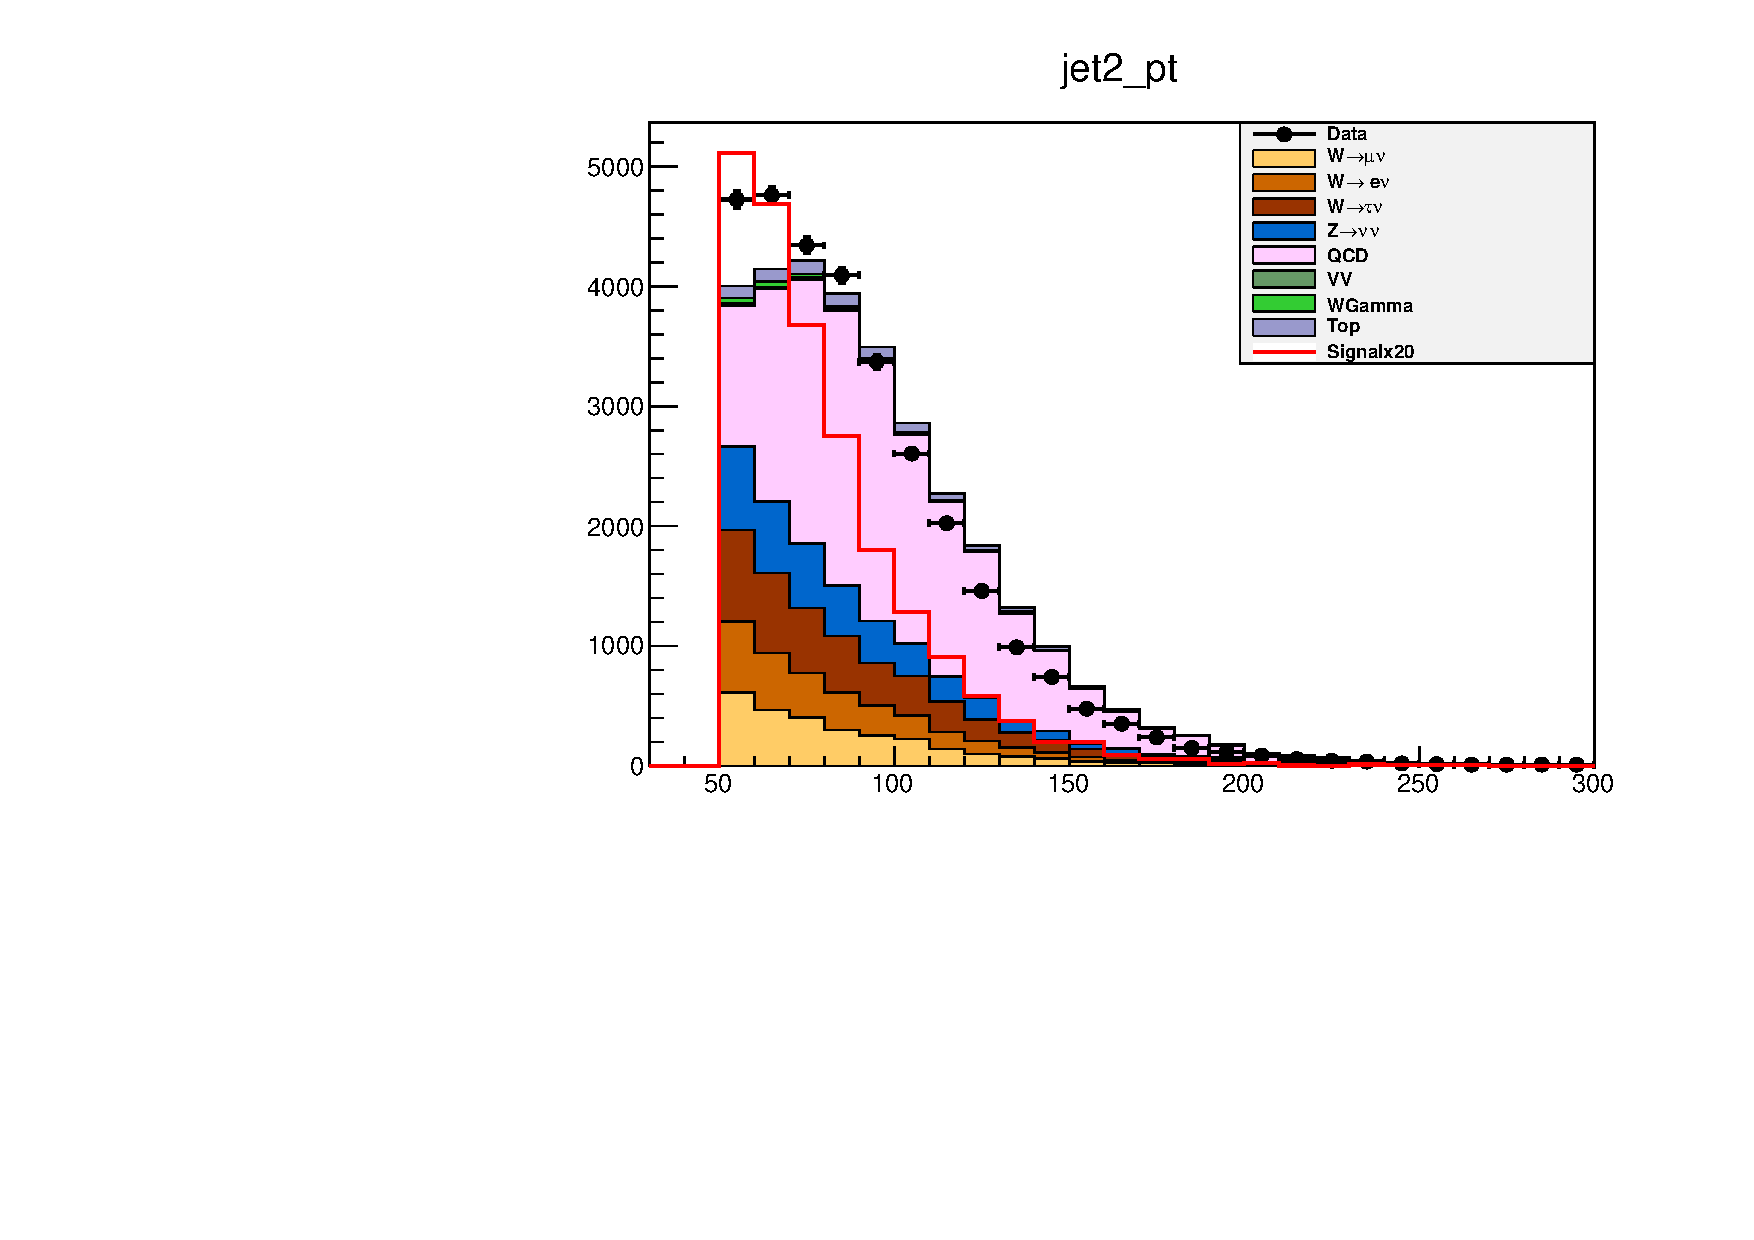
\includegraphics[width=\textwidth]{TalkPics/trigeffprog120814/nometmjjcutsig_jet2pt.pdf}
    \end{block}

  \end{columns}
\end{frame}

\begin{frame}
  \frametitle{New control plots}
  \begin{columns}
    \column{.5\textwidth}
    \begin{block}{METnomu}
      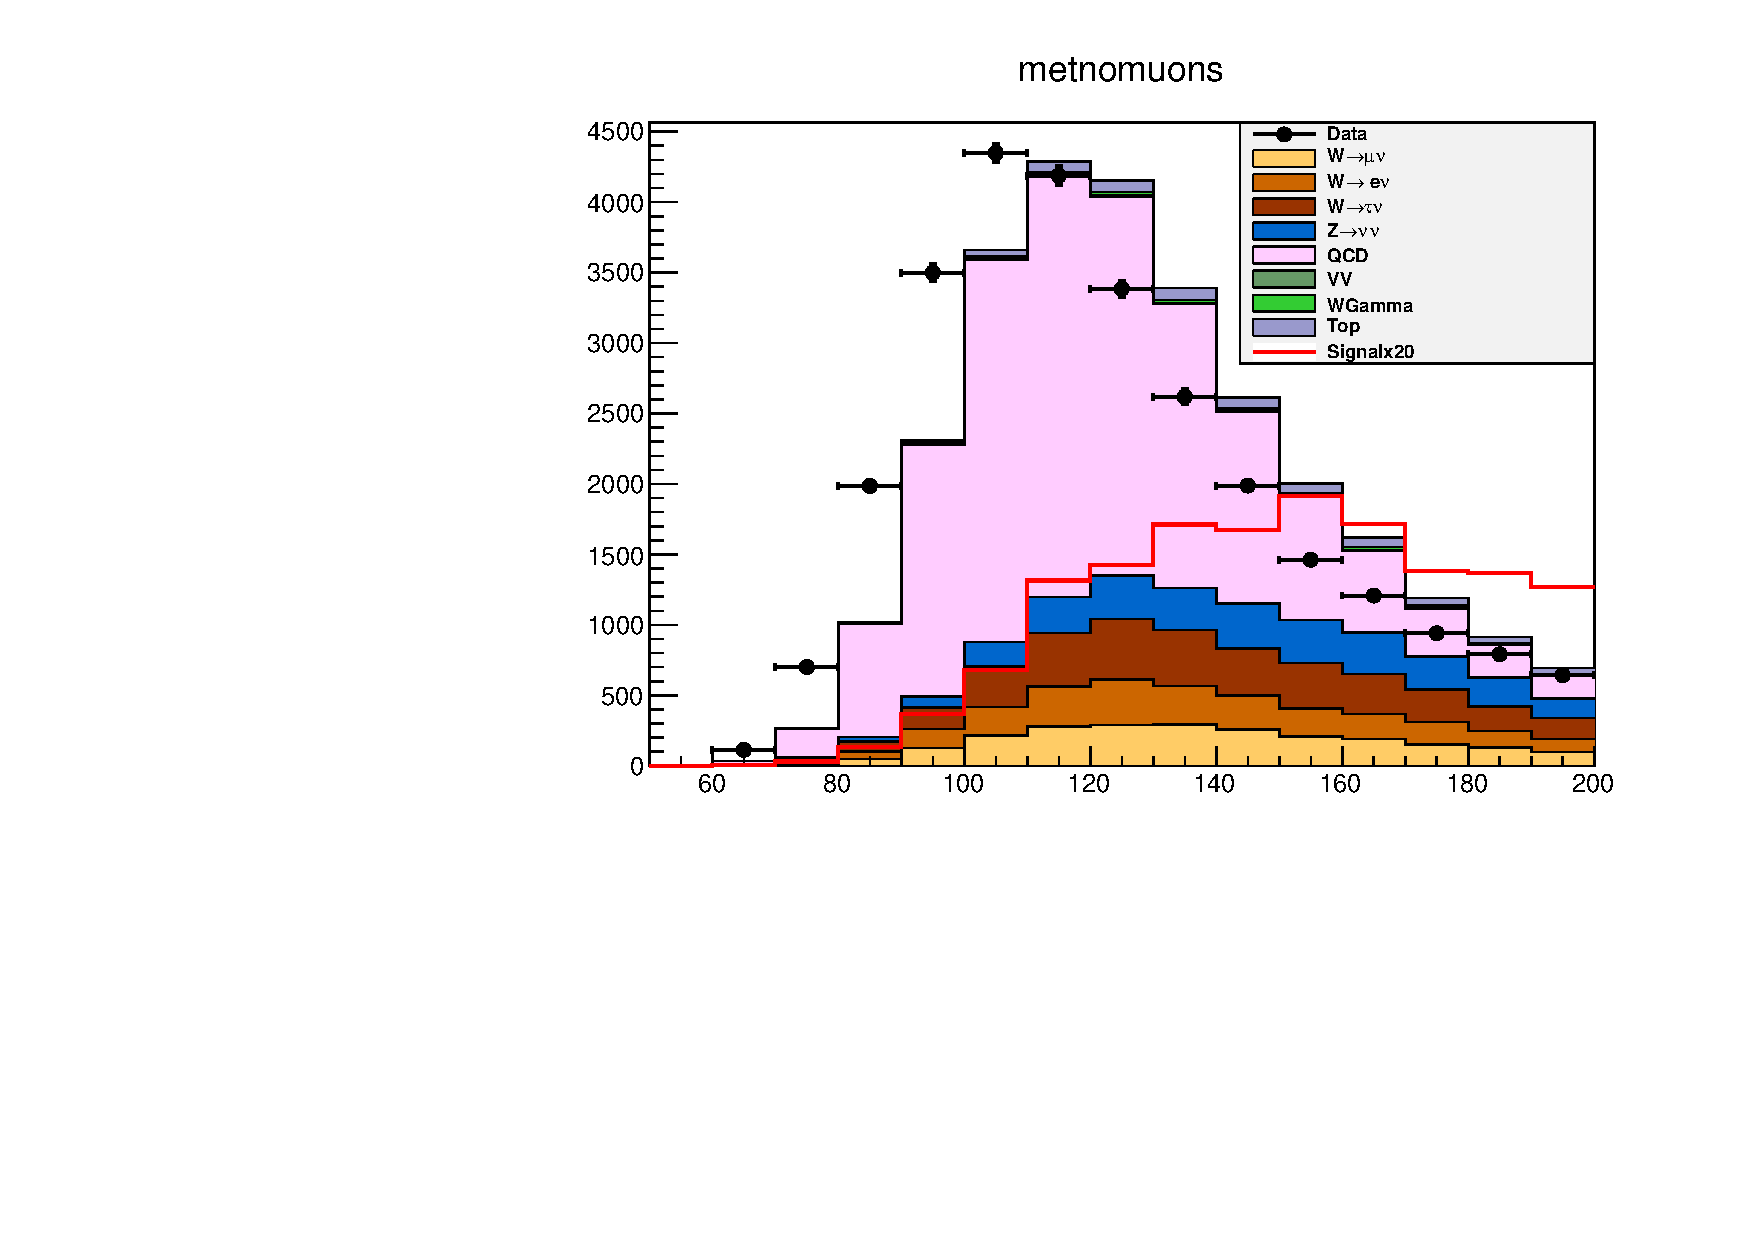
\includegraphics[width=\textwidth]{TalkPics/trigeffprog120814/nometmjjcutsig_metnomu.pdf}
    \end{block}
    \column{.5\textwidth}
    \begin{block}{METnomusig}
      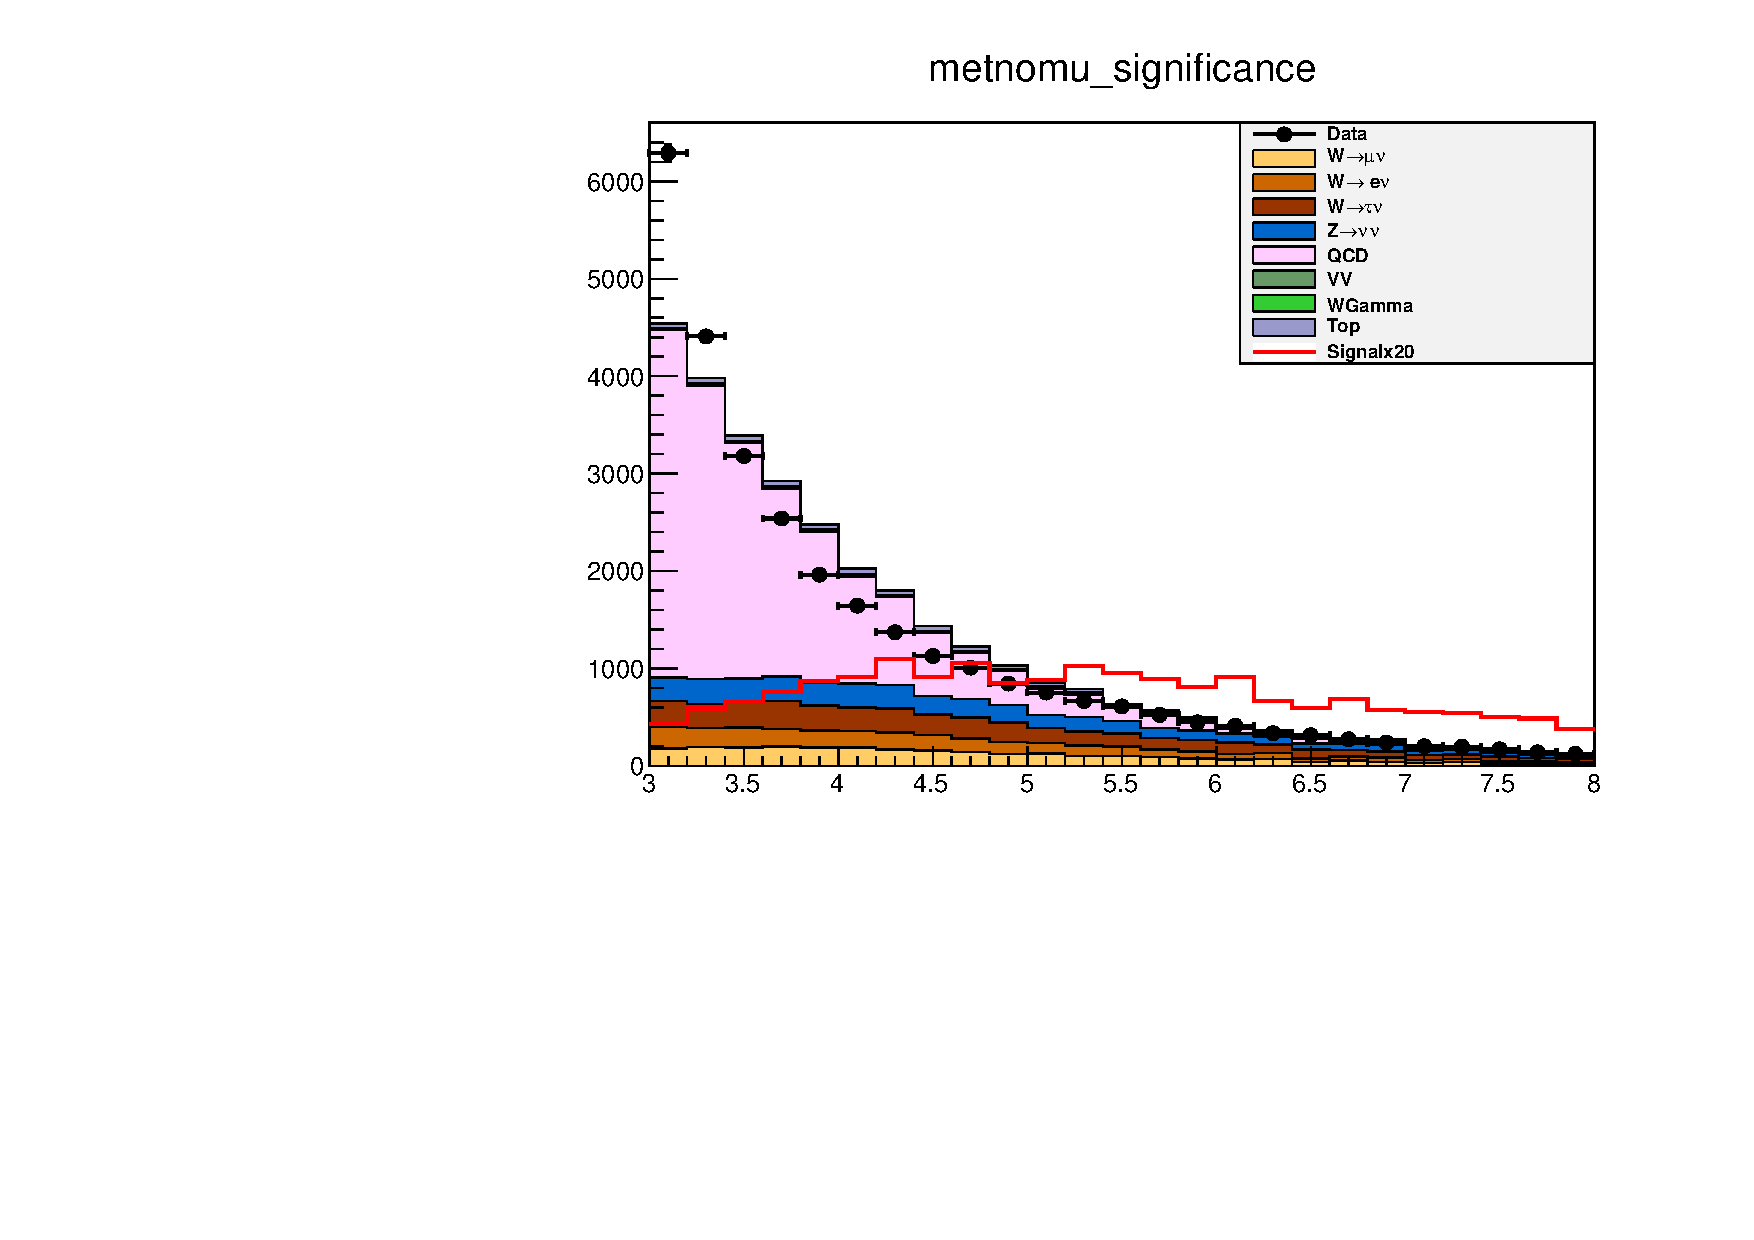
\includegraphics[width=\textwidth]{TalkPics/trigeffprog120814/nometmjjcutsig_metnomusig.pdf}
    \end{block}

  \end{columns}
\end{frame}

\begin{frame}
  \frametitle{New control plots}
  \begin{columns}
    \column{.5\textwidth}
    \begin{block}{Mjj}
      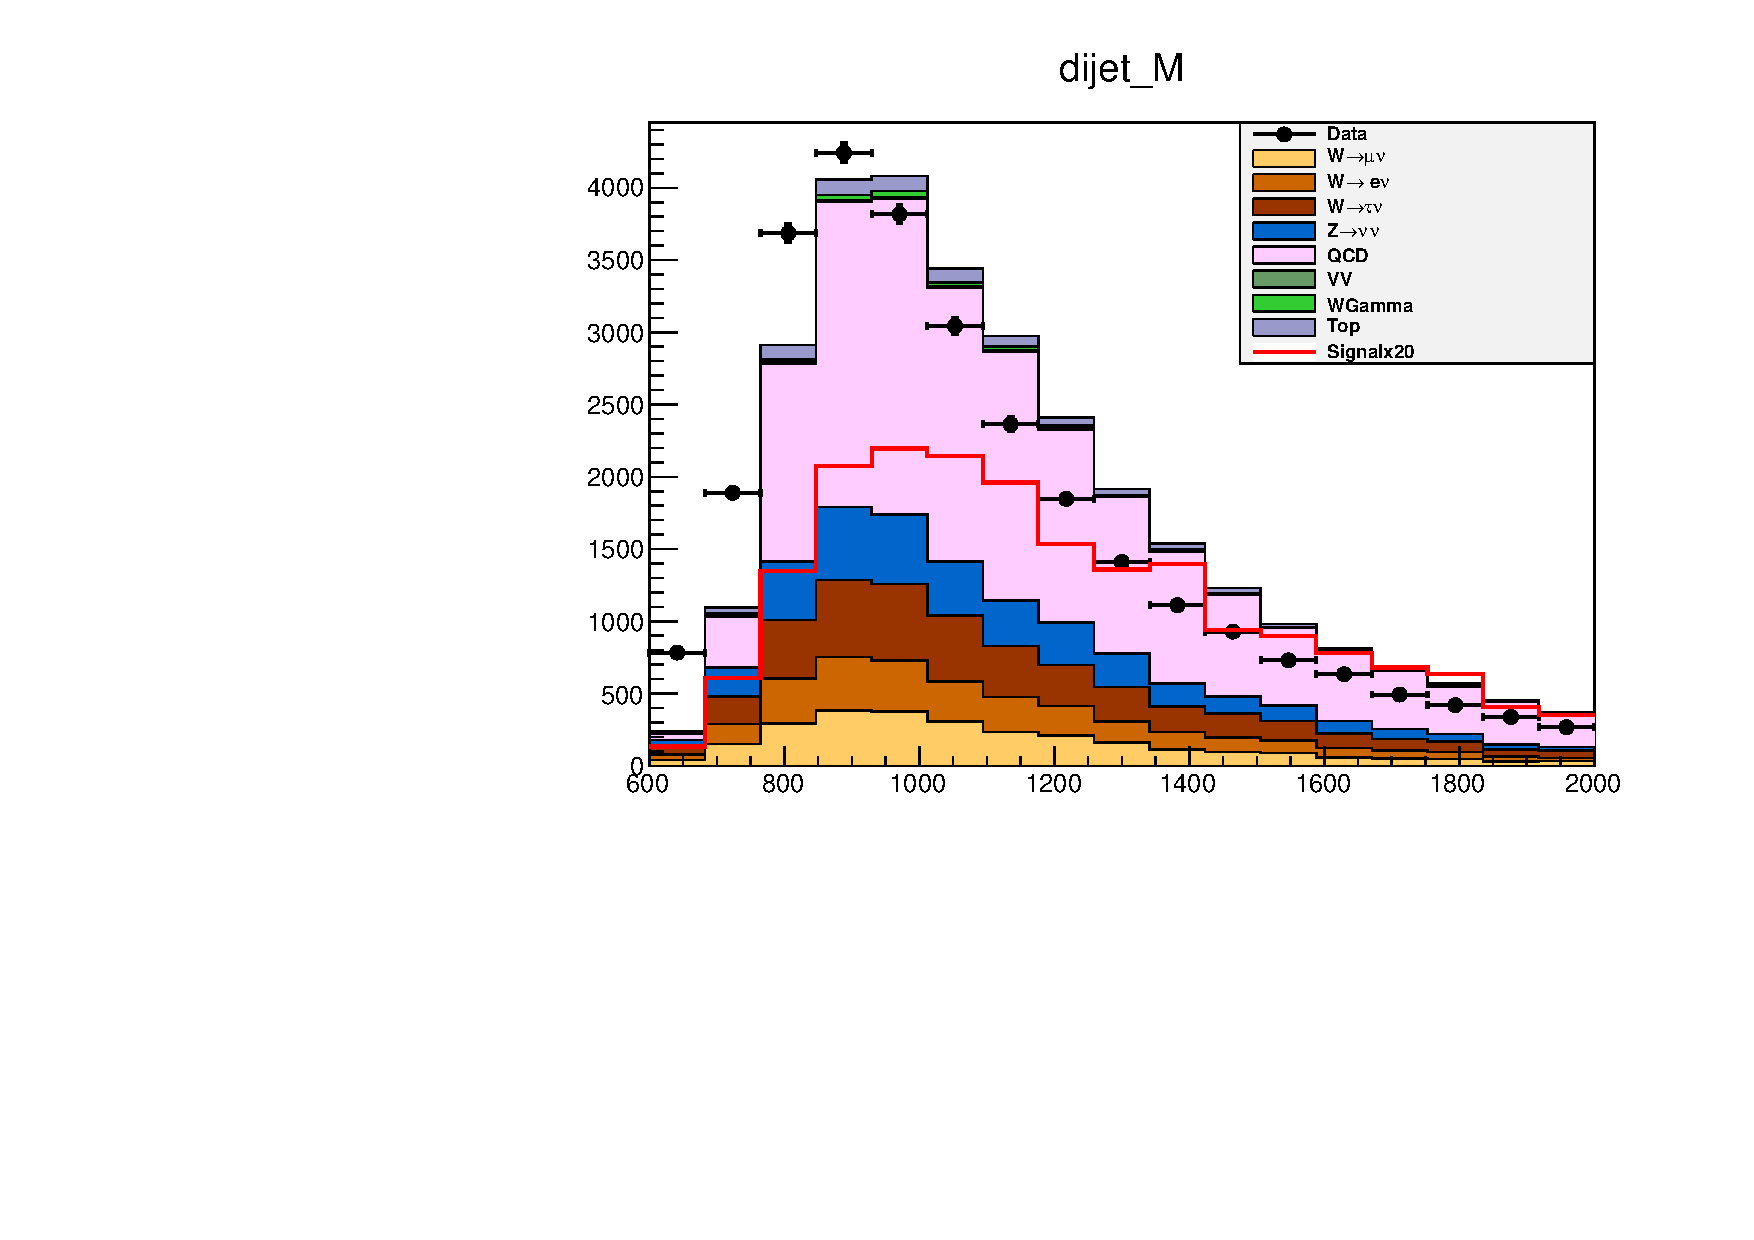
\includegraphics[width=\textwidth]{TalkPics/trigeffprog120814/nometmjjcutsig_mjj.pdf}
    \end{block}
    \column{.5\textwidth}
  \end{columns}
\end{frame}

\begin{frame}
  \frametitle{New control plots}
  \begin{columns}
    \column{.5\textwidth}
    \begin{block}{Dphijj}
      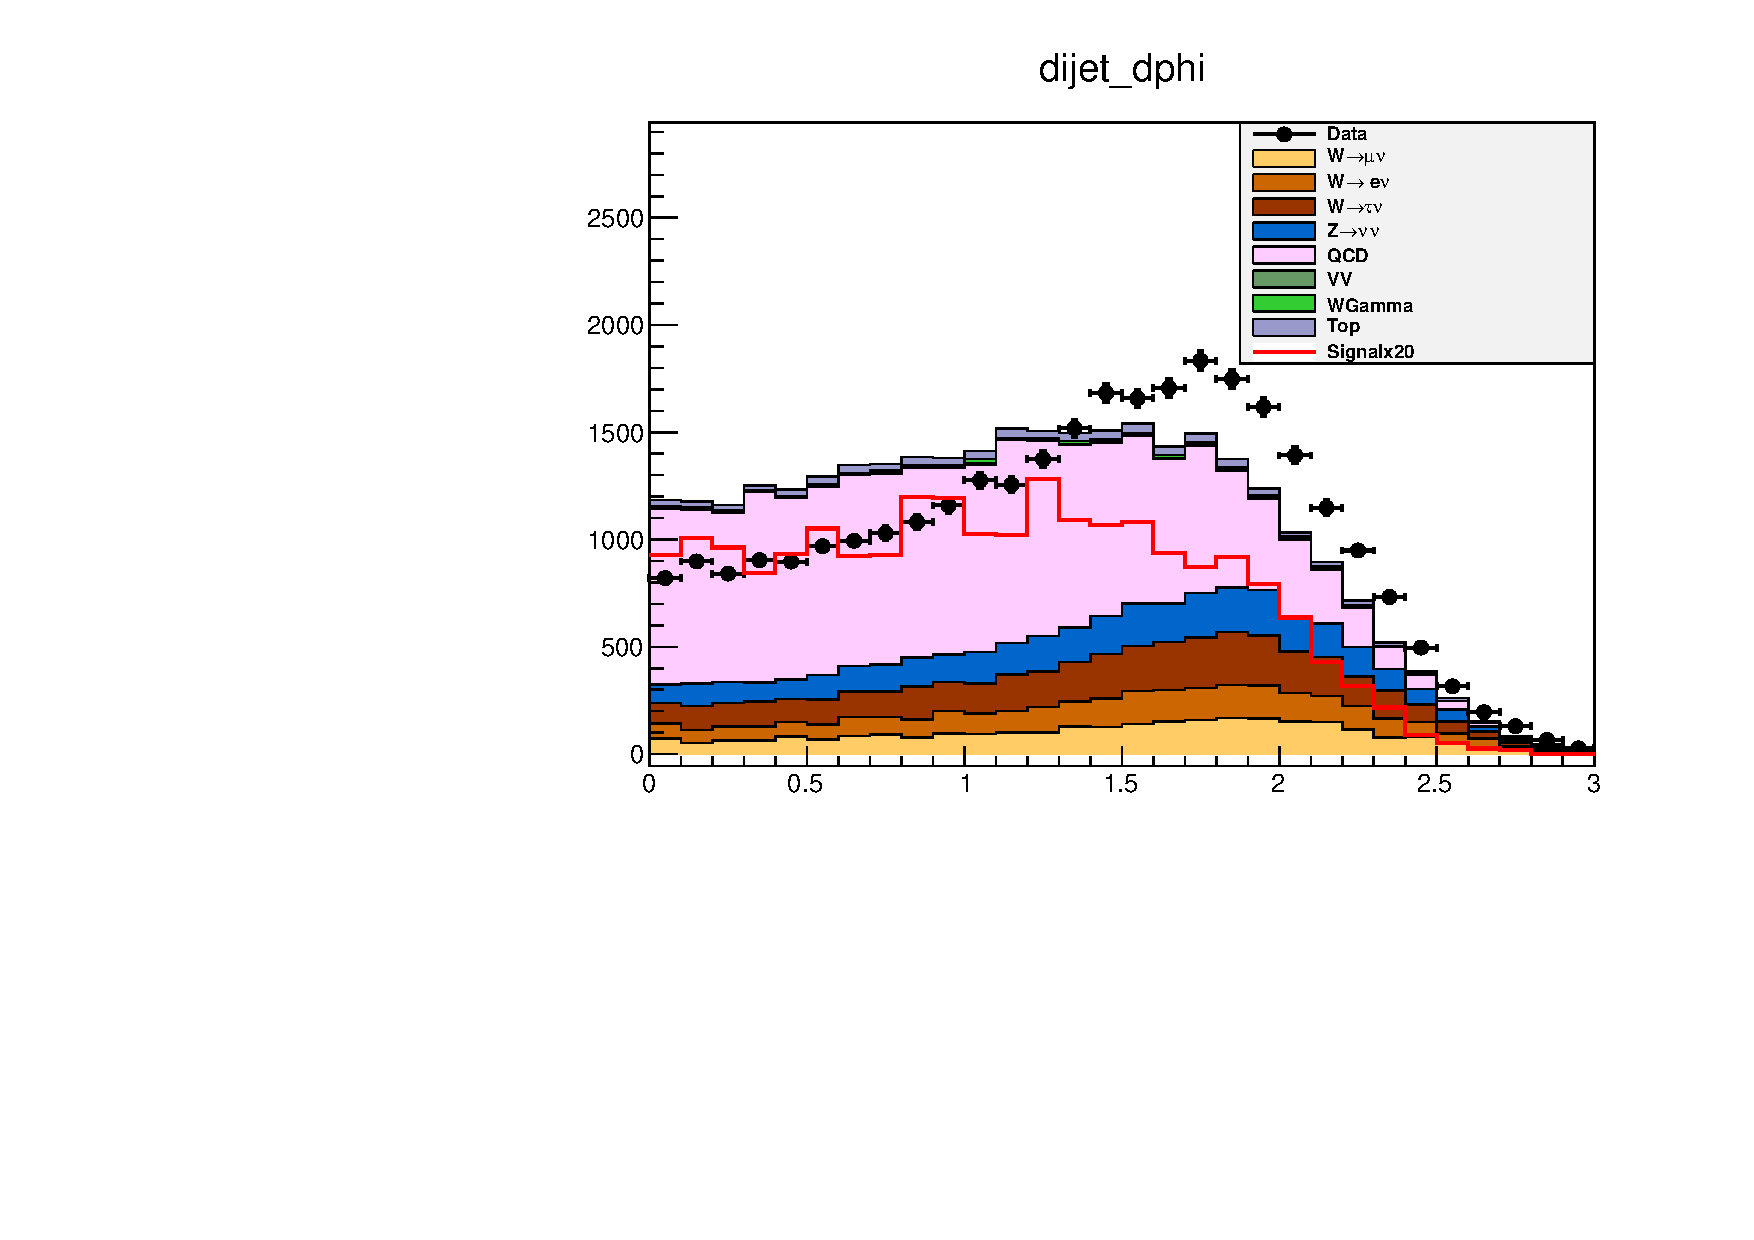
\includegraphics[width=\textwidth]{TalkPics/trigeffprog120814/nometmjjcutsig_dphijj.pdf}
    \end{block}
    \column{.5\textwidth}
    \begin{block}{Detajj}
      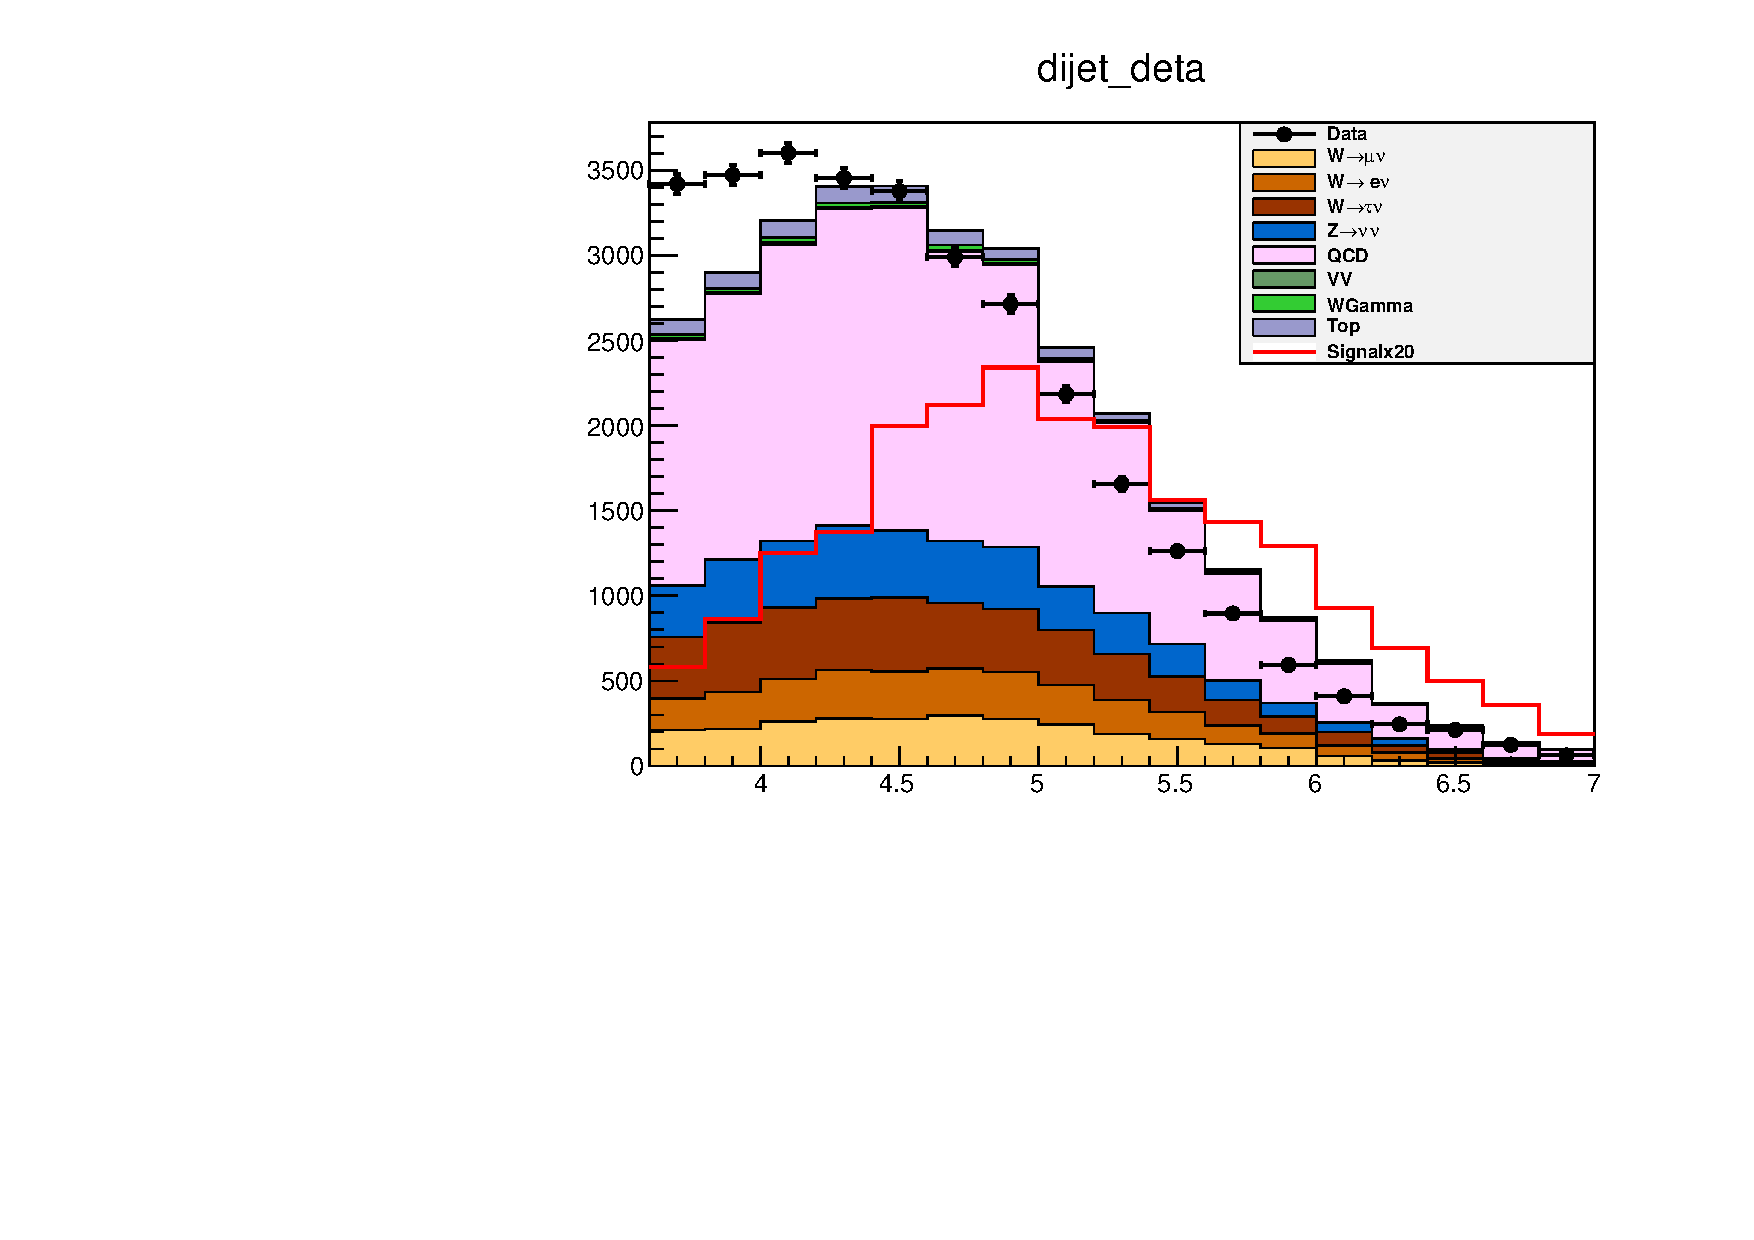
\includegraphics[width=\textwidth]{TalkPics/trigeffprog120814/nometmjjcutsig_detajj.pdf}
    \end{block}

  \end{columns}
\end{frame}

\begin{frame}
  \frametitle{New control plots}
  \begin{columns}
    \column{.5\textwidth}
    \begin{block}{Jet-met mindphi}
      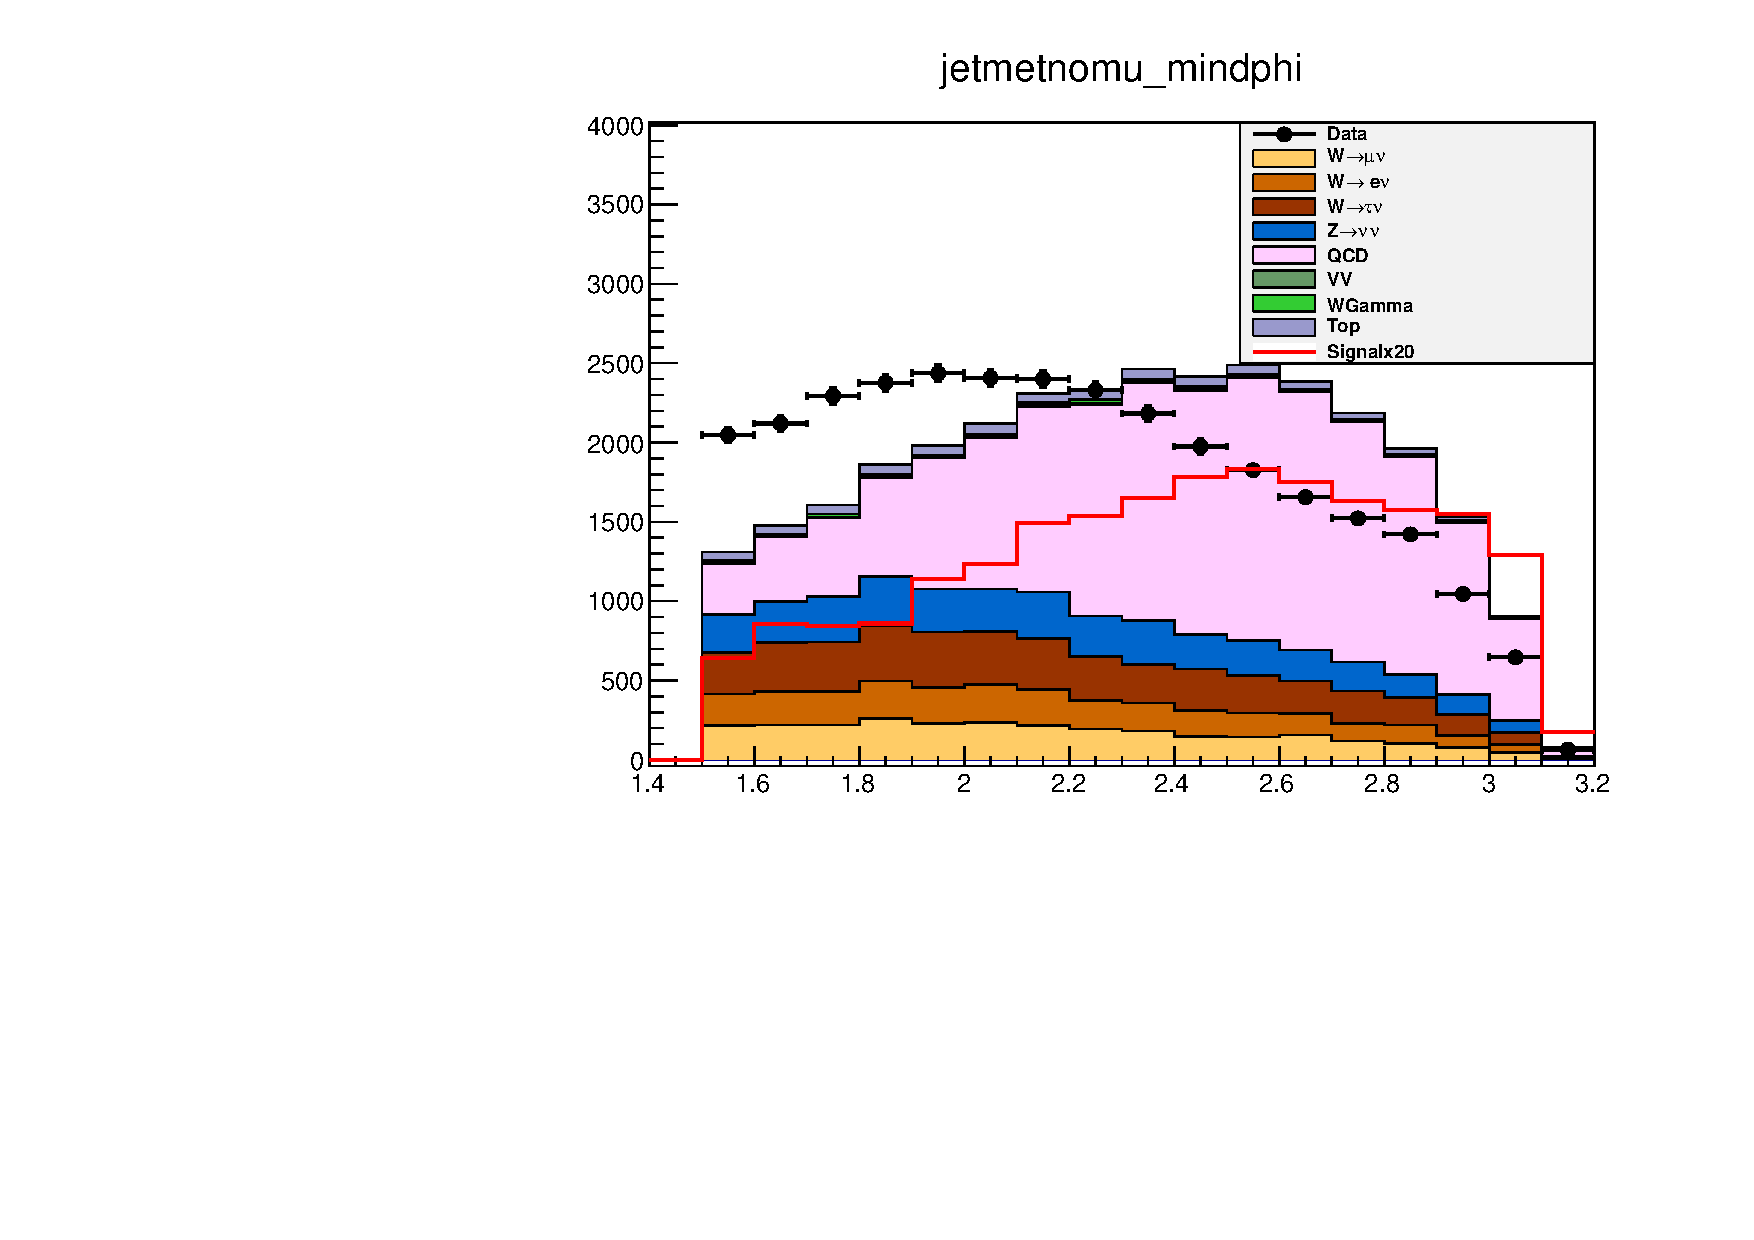
\includegraphics[width=\textwidth]{TalkPics/trigeffprog120814/nometmjjcutsig_jetmetmindphi.pdf}
    \end{block}
    \column{.5\textwidth}
    \begin{block}{dijet-metnomu pt fraction}
      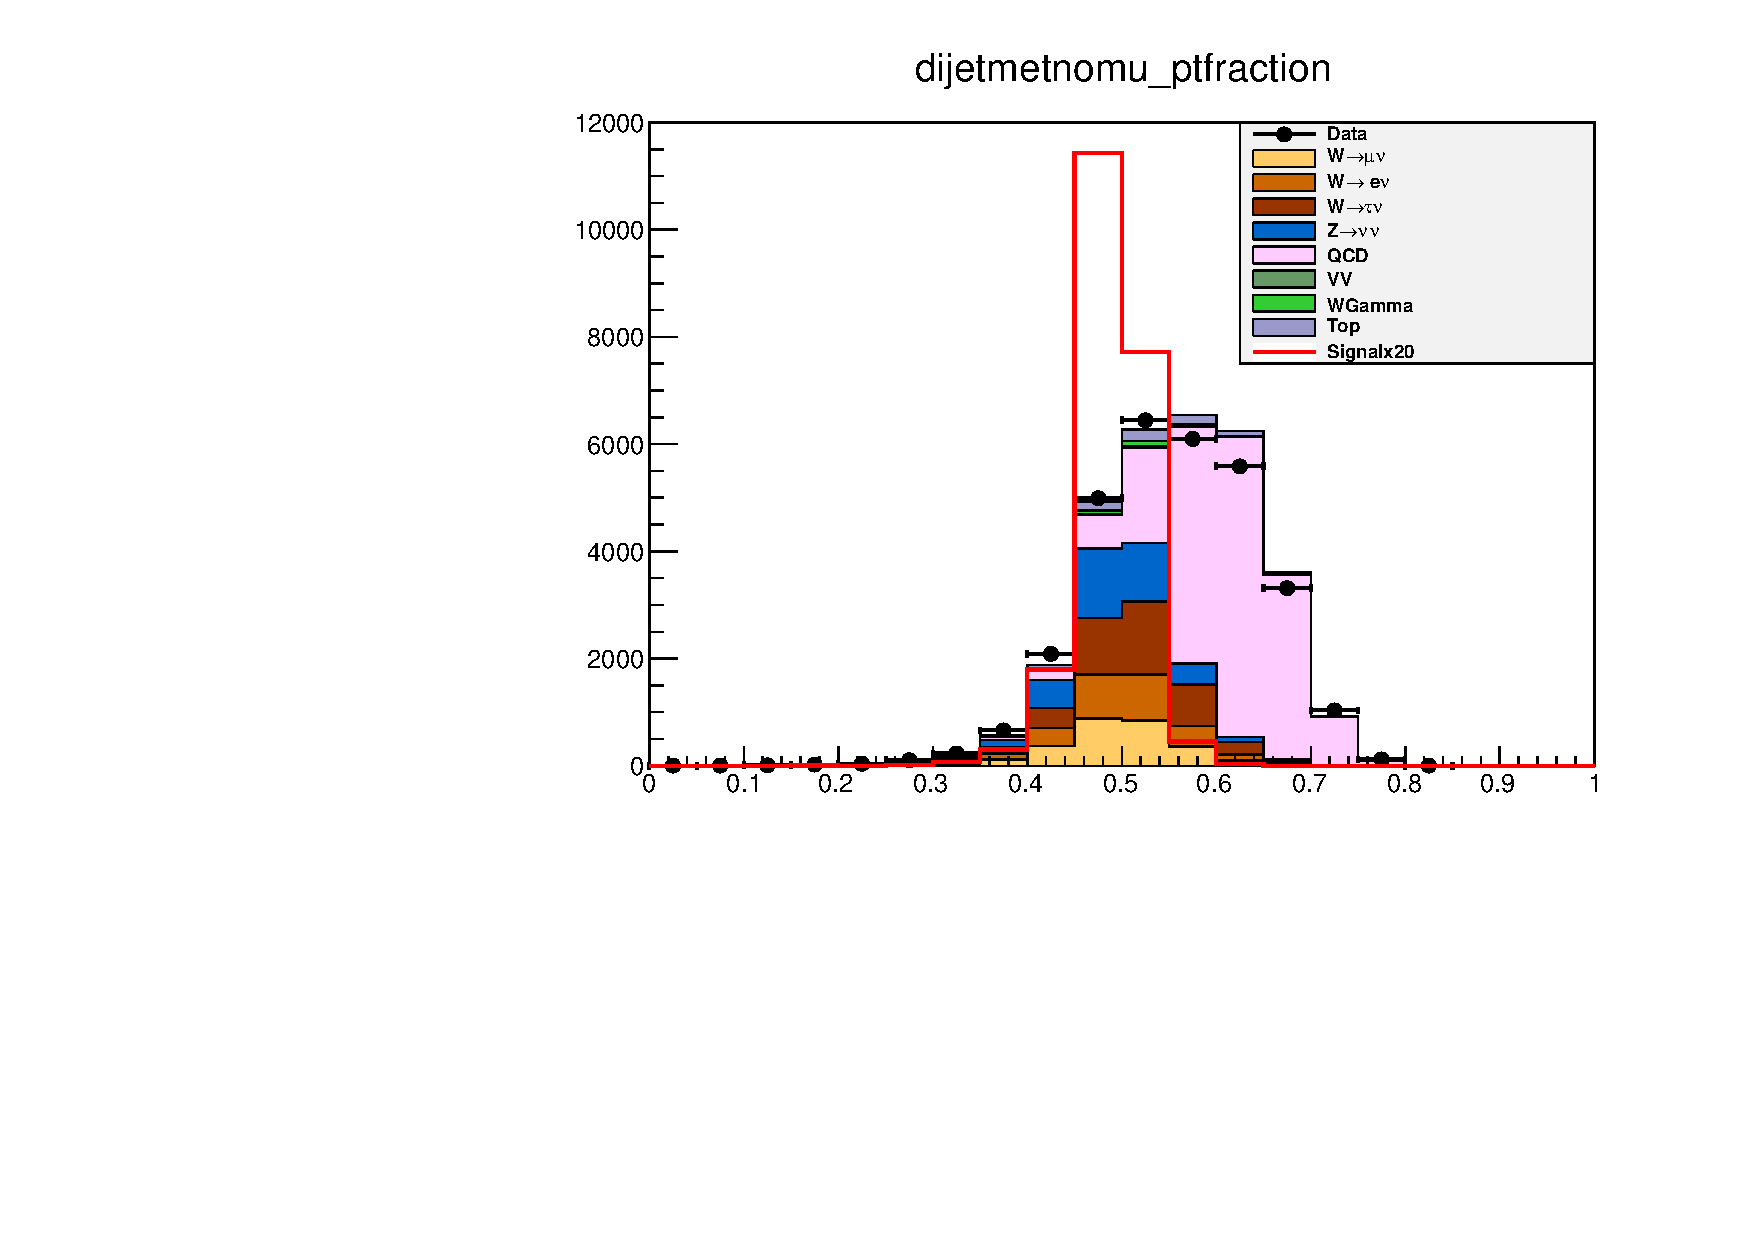
\includegraphics[width=\textwidth]{TalkPics/trigeffprog120814/nometmjjcutsig_dijetmetnomuptfrac.pdf}
    \end{block}

  \end{columns}
\end{frame}

\begin{frame}
  \frametitle{Control regions - Wmu}
  \begin{columns}
    \column{.5\textwidth}
    \begin{block}{Dphijj}
      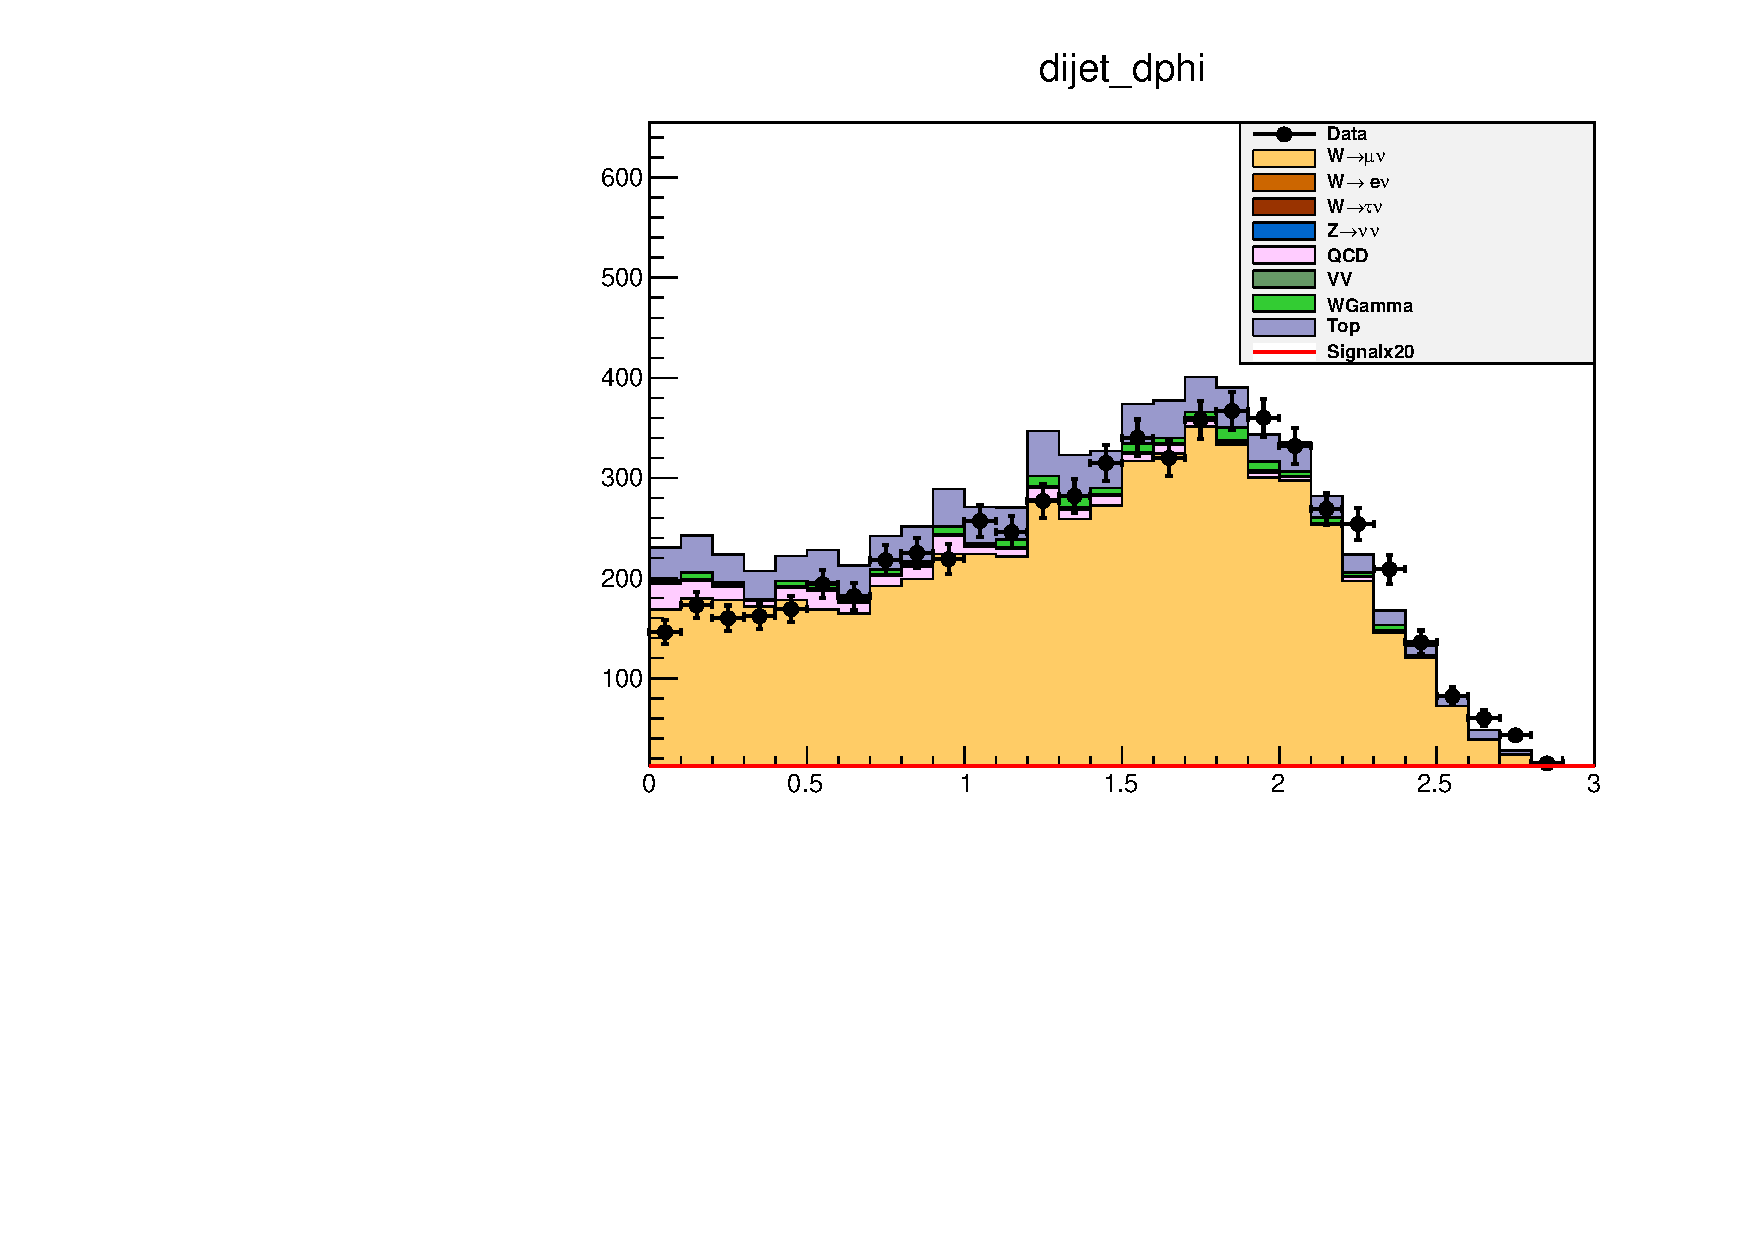
\includegraphics[width=\textwidth]{TalkPics/trigeffprog120814/wmu_dphijj.pdf}
    \end{block}
    \column{.5\textwidth}
    \begin{block}{Jet-MET mindphi}
      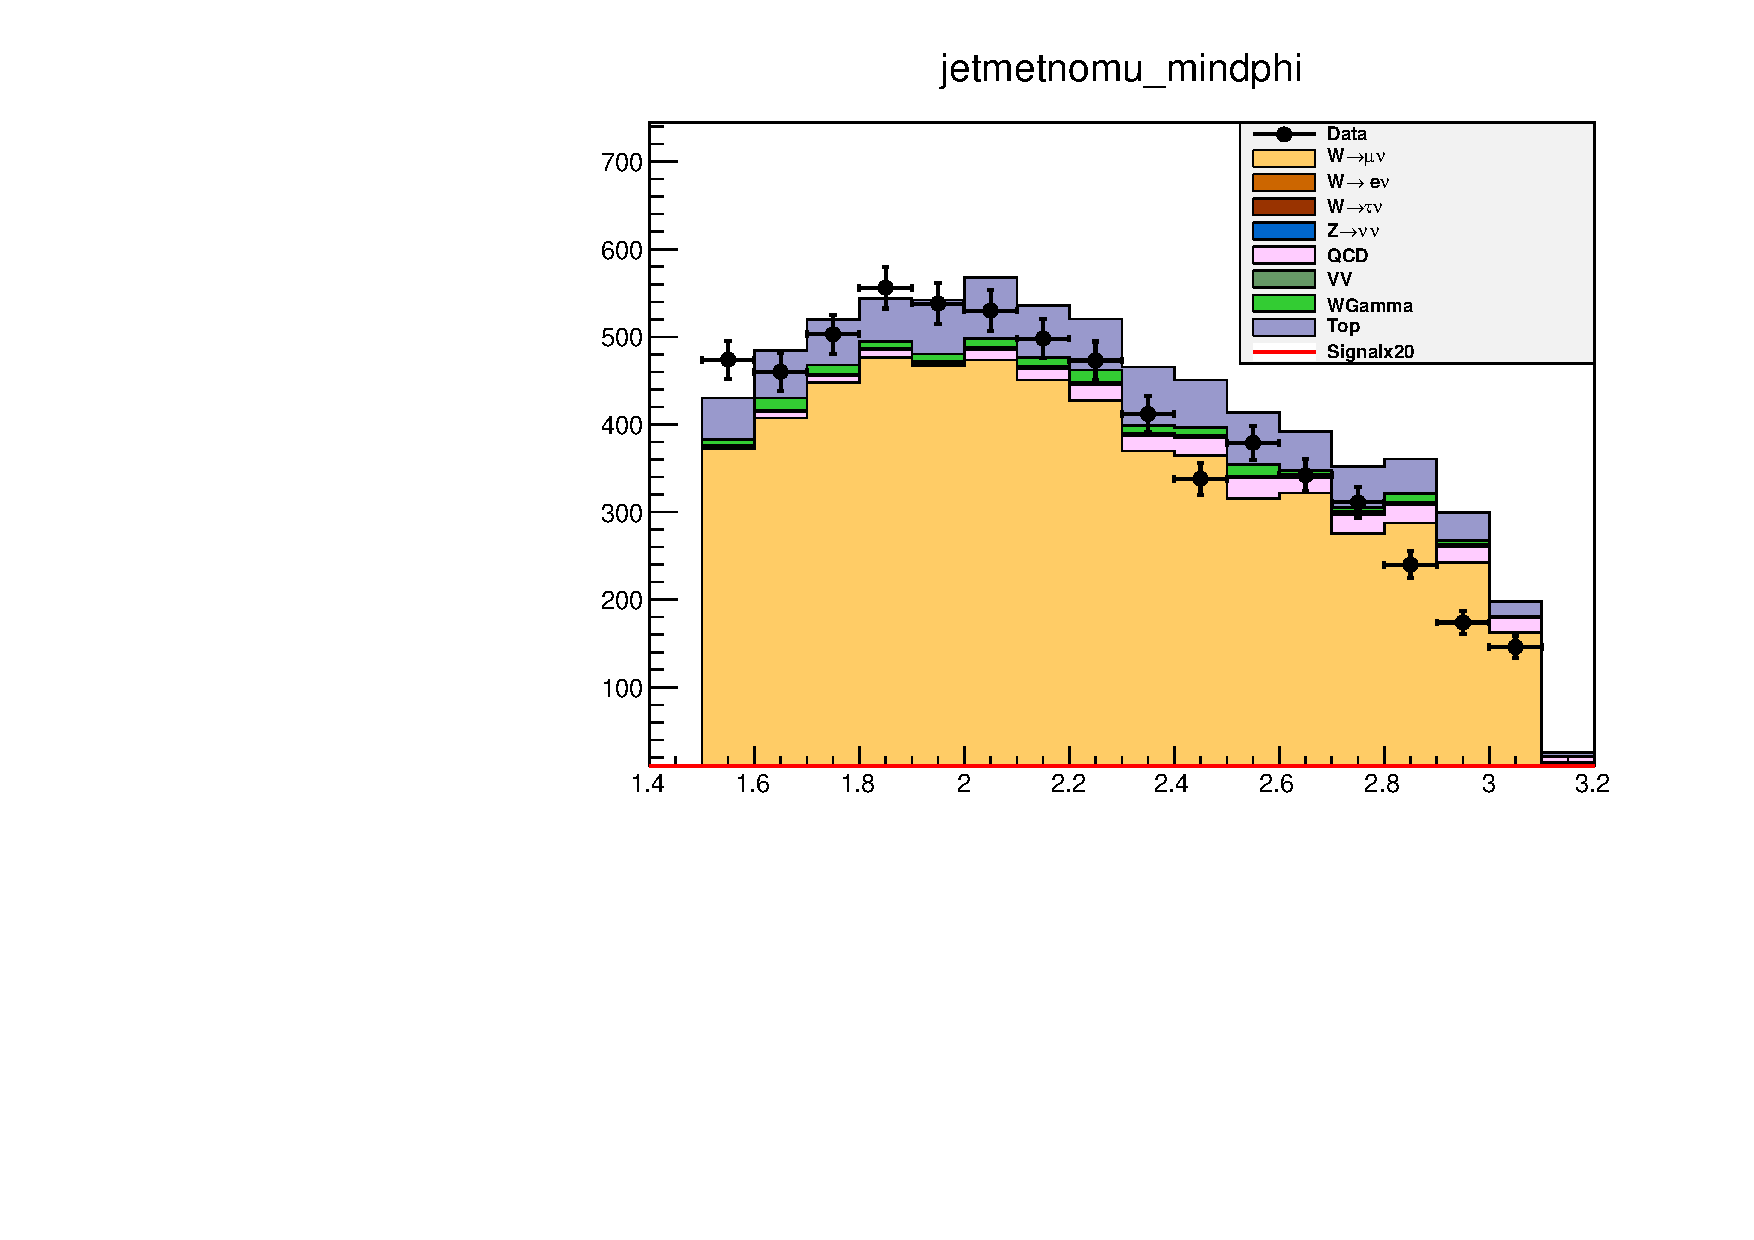
\includegraphics[width=\textwidth]{TalkPics/trigeffprog120814/wmu_jetmetmindphi.pdf}
    \end{block}

  \end{columns}
\end{frame}

\begin{frame}
  \frametitle{Control regions - Wel}
  \begin{columns}
    \column{.5\textwidth}
    \begin{block}{Dphijj}
      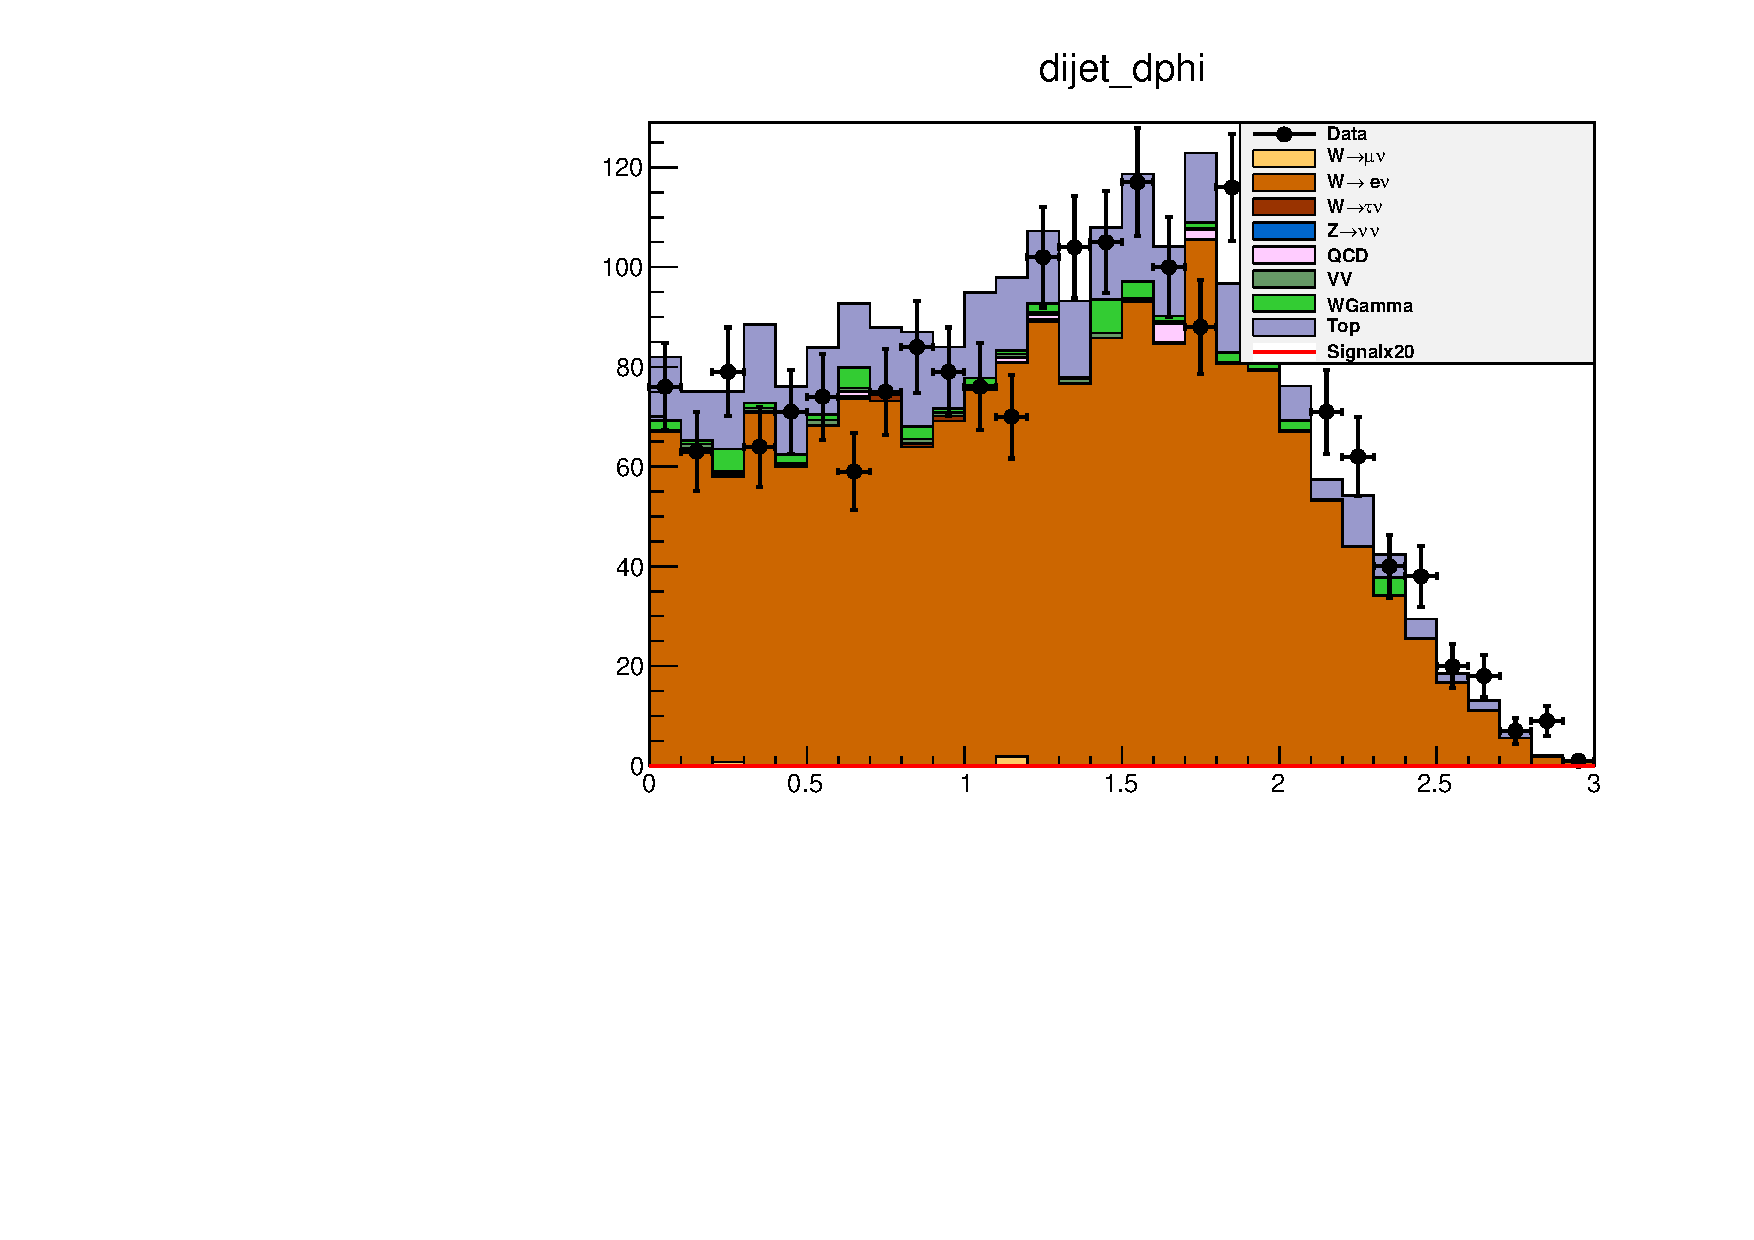
\includegraphics[width=\textwidth]{TalkPics/trigeffprog120814/wel_dphijj.pdf}
    \end{block}
    \column{.5\textwidth}
    \begin{block}{Jet-MET mindphi}
      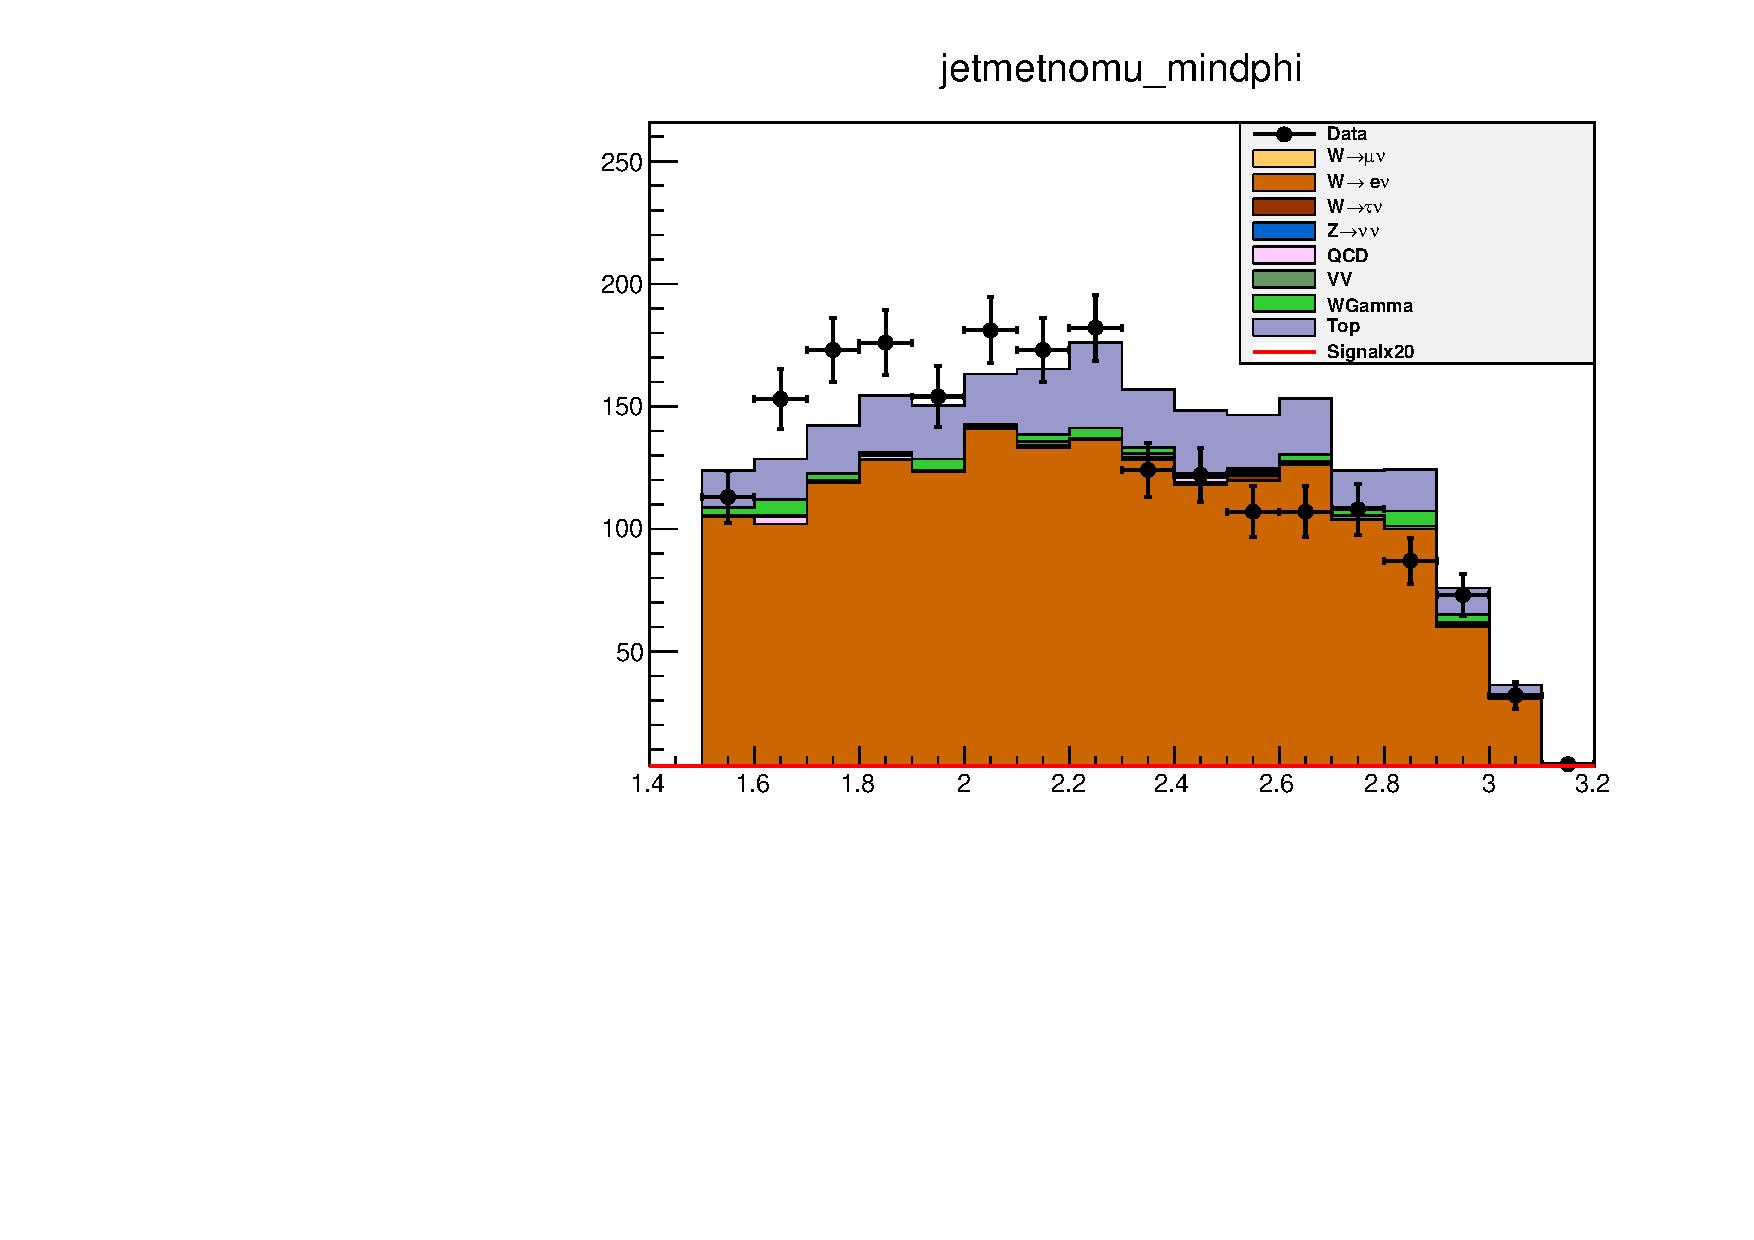
\includegraphics[width=\textwidth]{TalkPics/trigeffprog120814/wel_jetmetmindphi.pdf}
    \end{block}

  \end{columns}
\end{frame}

\begin{frame}
  \frametitle{Control regions - Wtau}
  \begin{columns}
    \column{.5\textwidth}
    \begin{block}{Dphijj}
      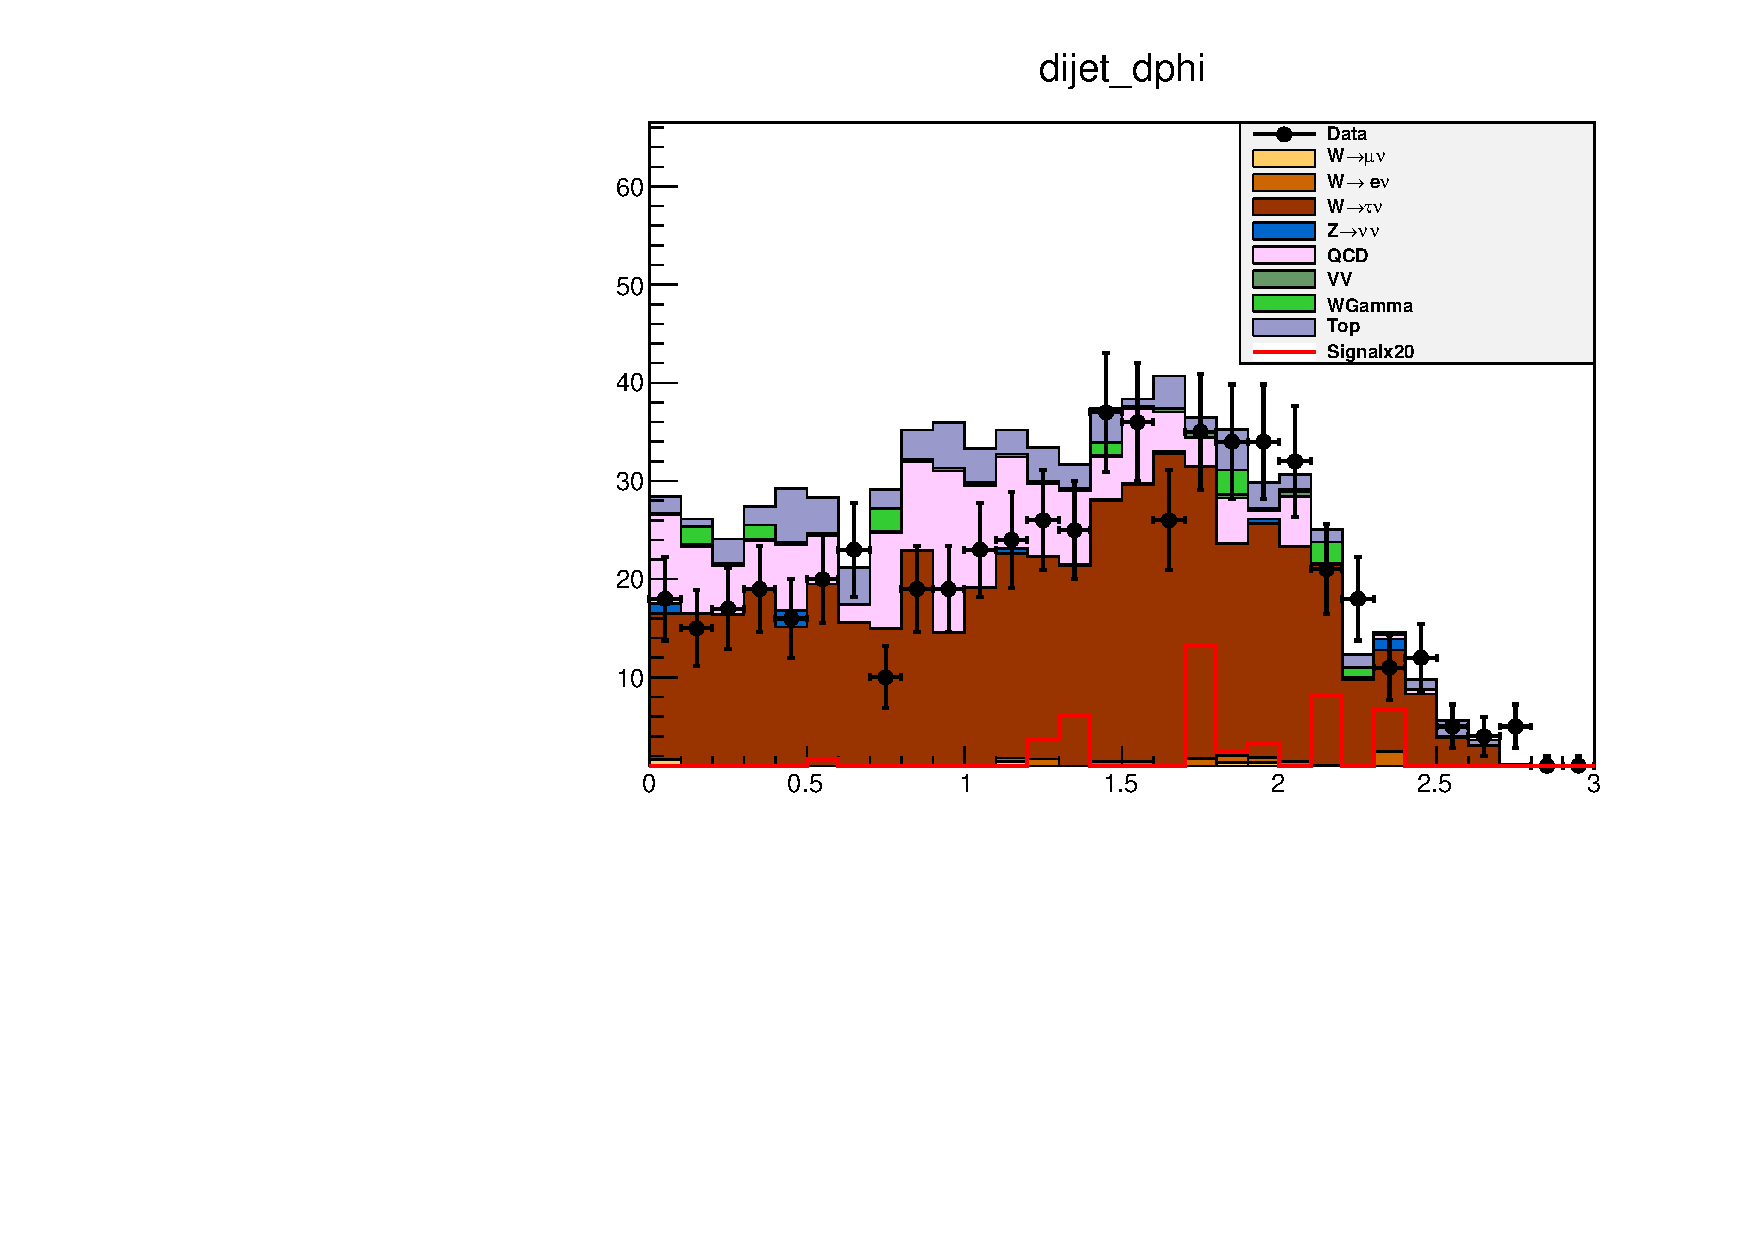
\includegraphics[width=\textwidth]{TalkPics/trigeffprog120814/wtau_dphijj.pdf}
    \end{block}
    \column{.5\textwidth}
    \begin{block}{Jet-MET mindphi}
      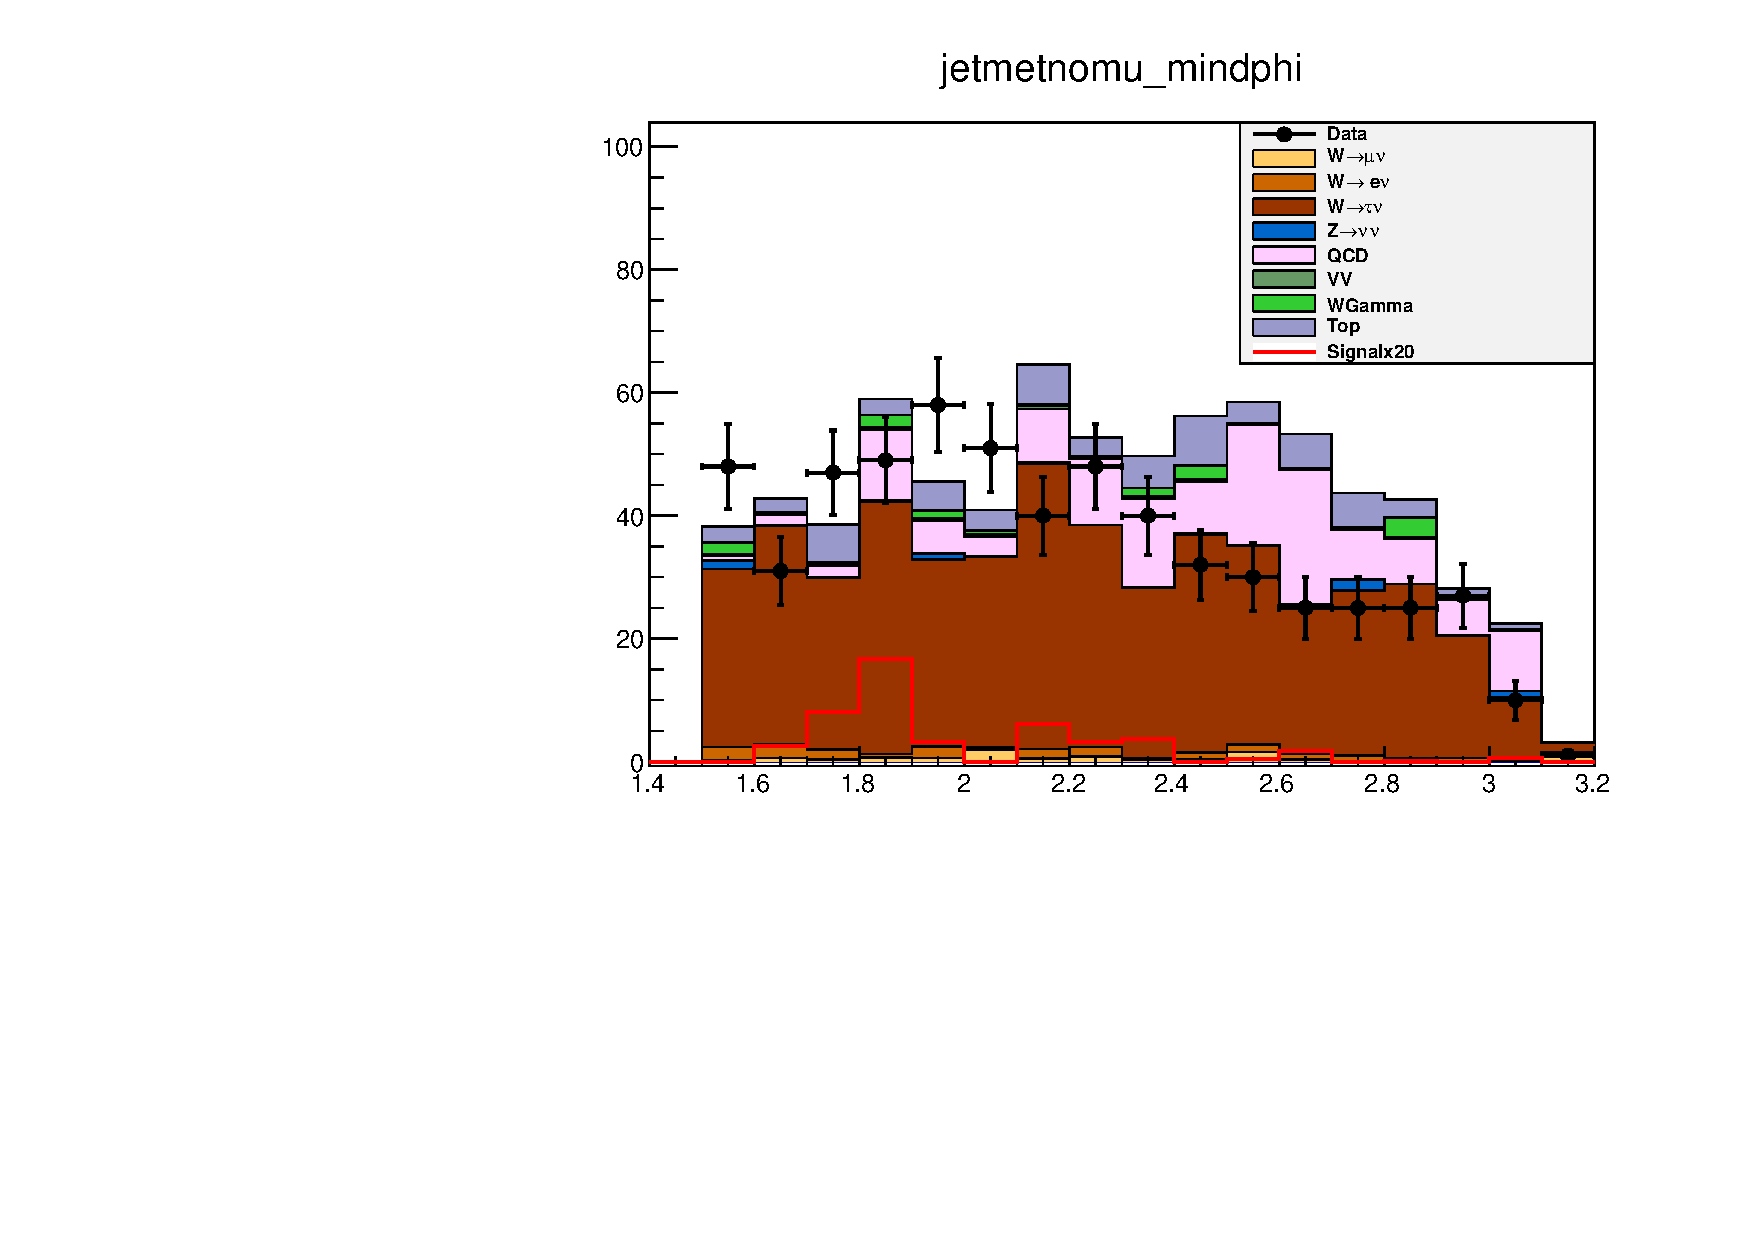
\includegraphics[width=\textwidth]{TalkPics/trigeffprog120814/wtau_jetmetmindphi.pdf}
    \end{block}

  \end{columns}
\end{frame}

\begin{frame}
  \frametitle{Control regions - Zmumu}
  \begin{columns}
    \column{.5\textwidth}
    \begin{block}{Dphijj}
      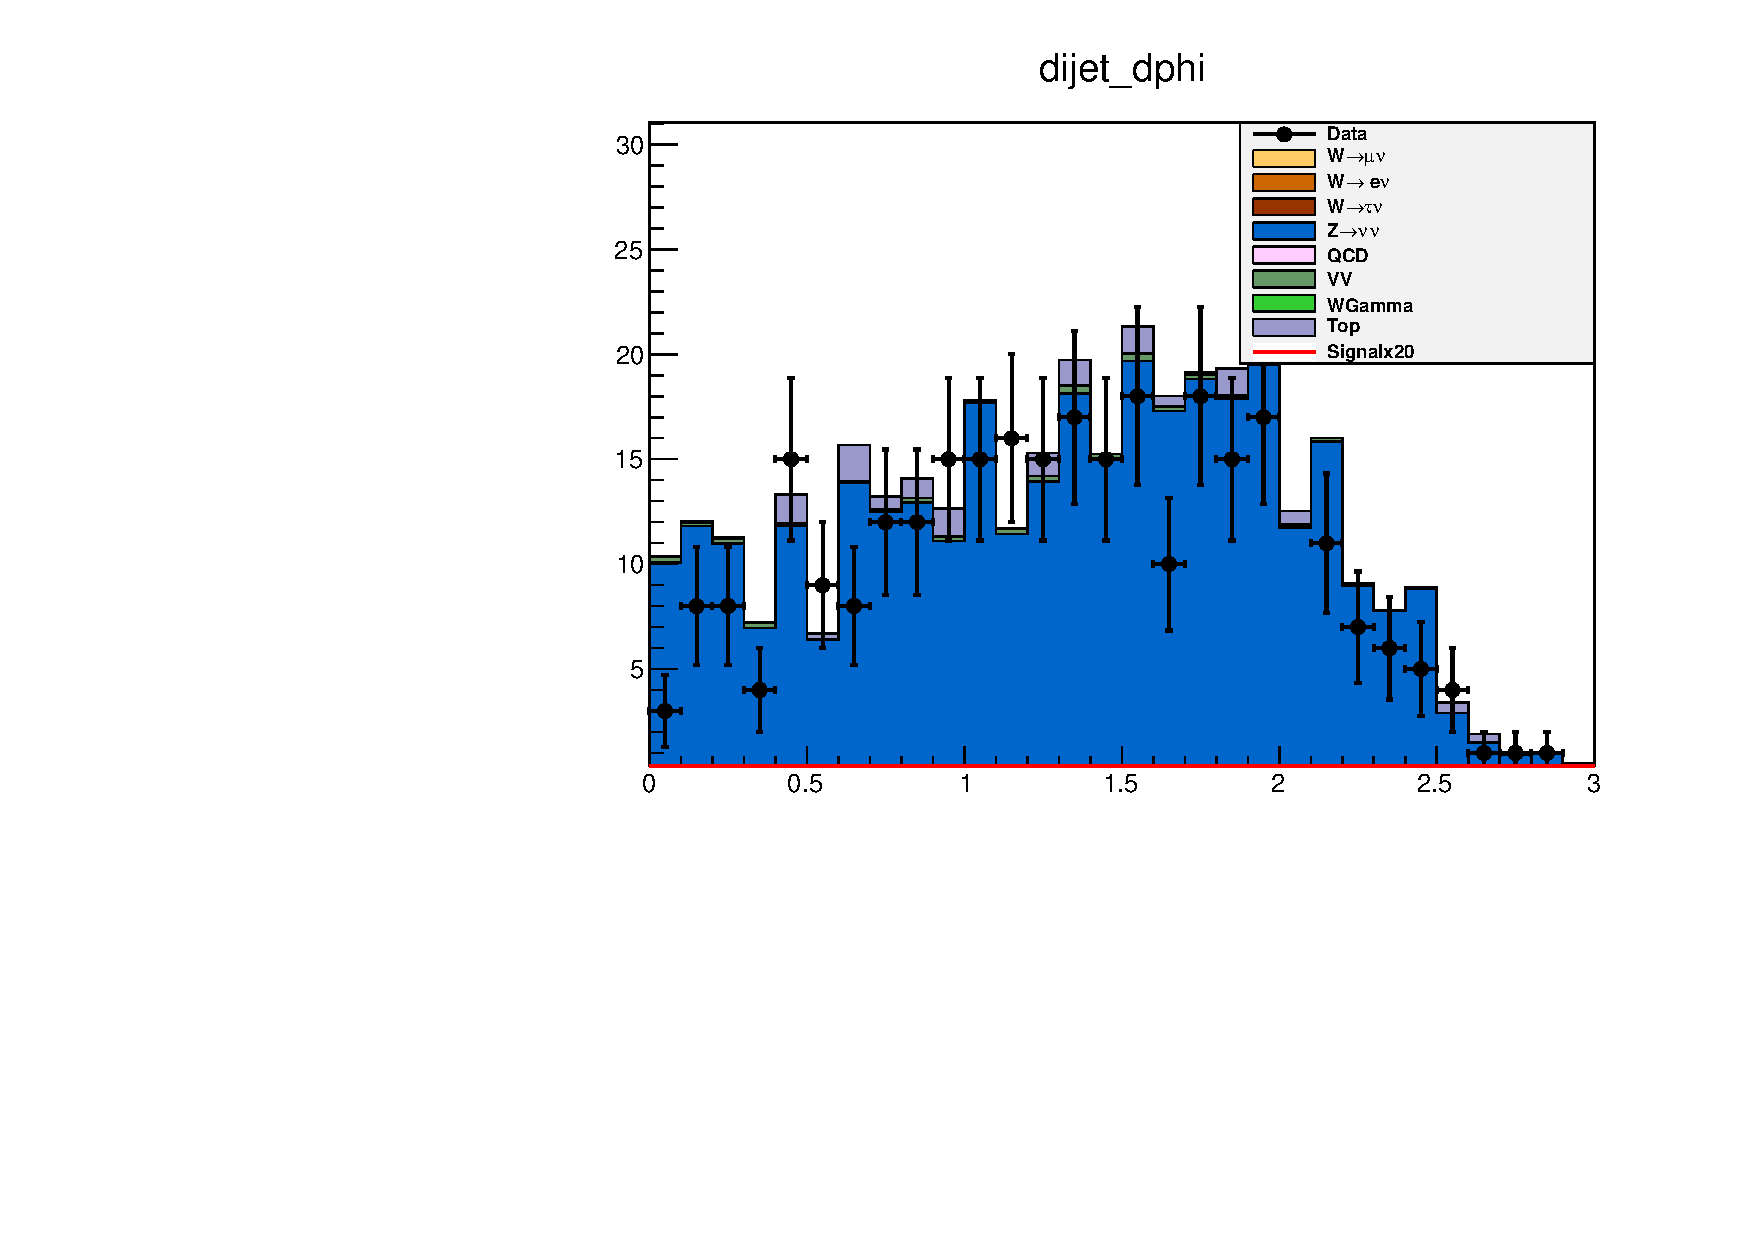
\includegraphics[width=\textwidth]{TalkPics/trigeffprog120814/zmumu_dphijj.pdf}
    \end{block}
    \column{.5\textwidth}
    \begin{block}{Jet-MET mindphi}
      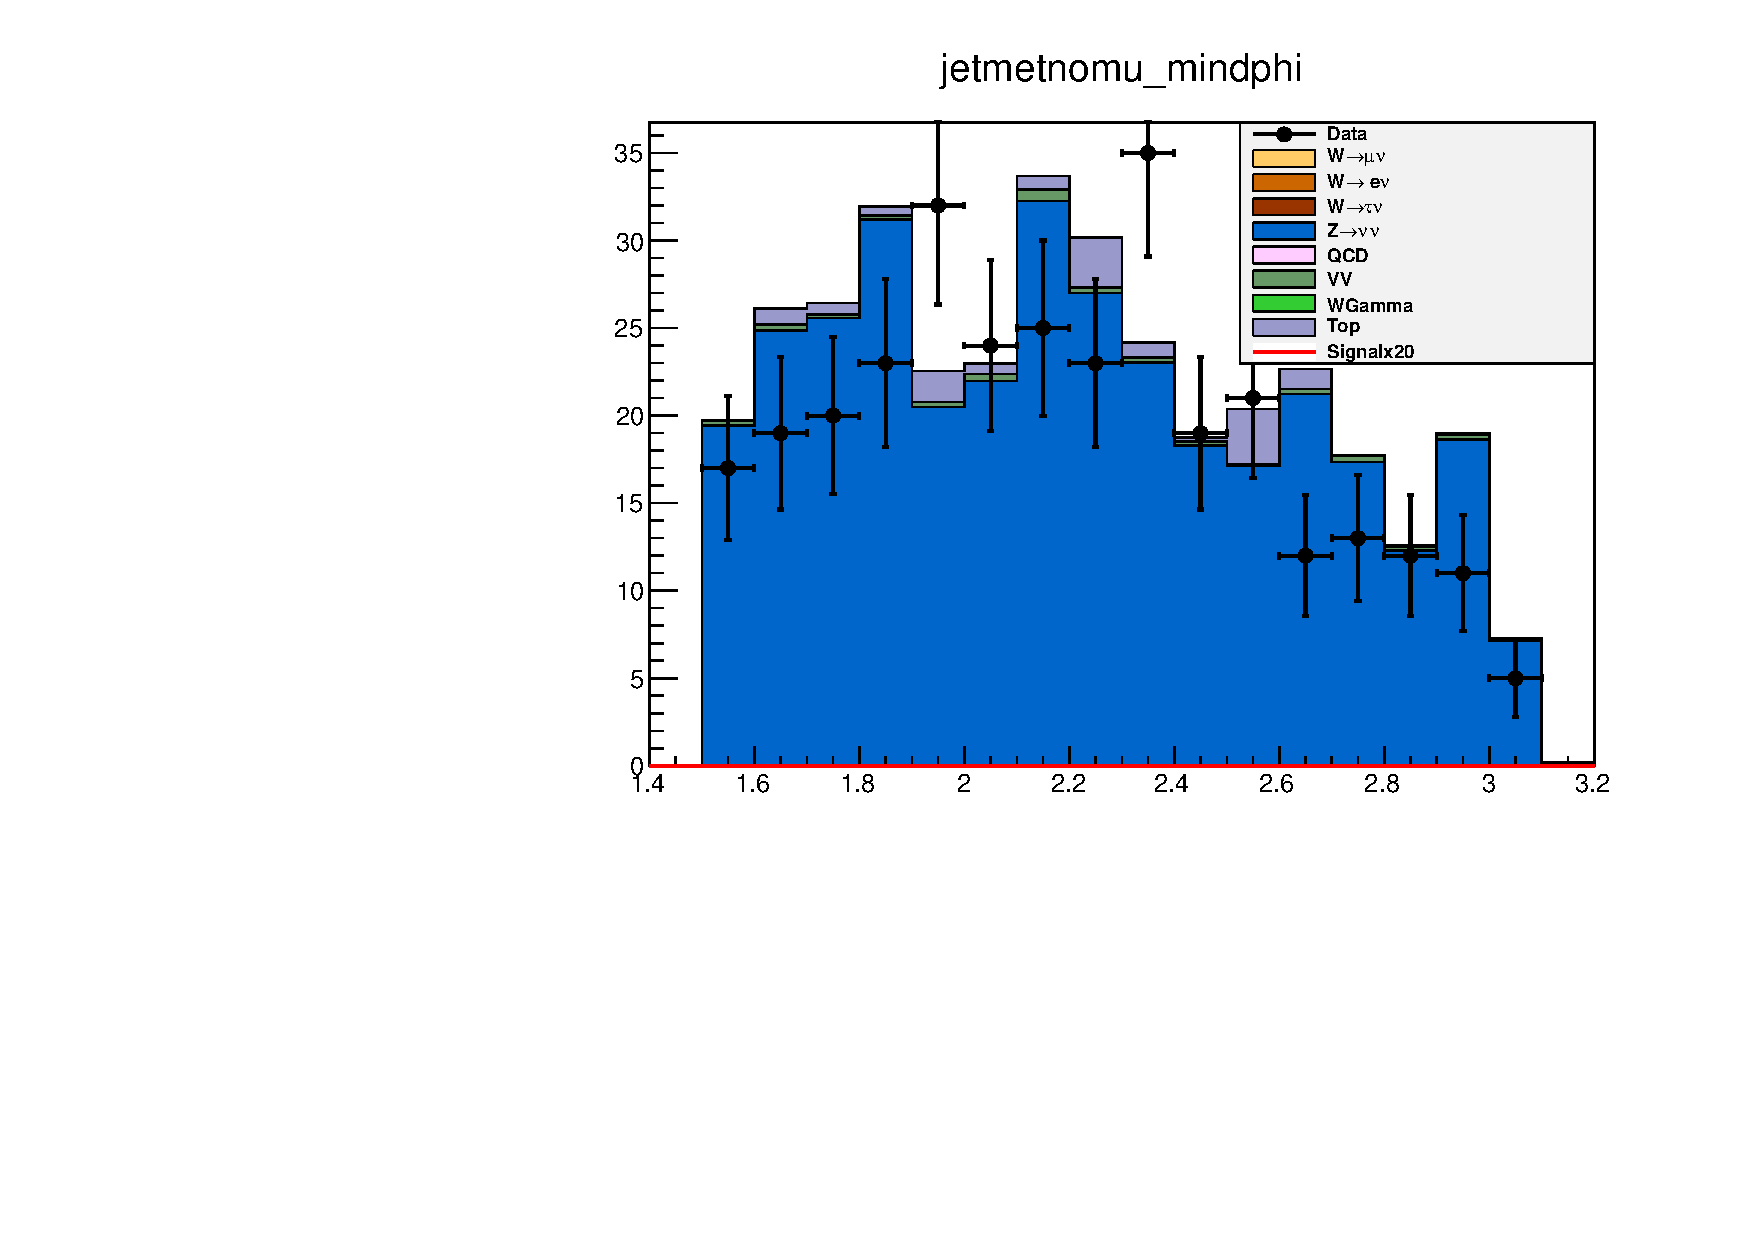
\includegraphics[width=\textwidth]{TalkPics/trigeffprog120814/zmumu_jetmetmindphi.pdf}
    \end{block}

  \end{columns}
\end{frame}

\begin{frame}
  \frametitle{Control regions - QCD}
  \begin{columns}
    \column{.5\textwidth}
    \begin{block}{Dphijj}
      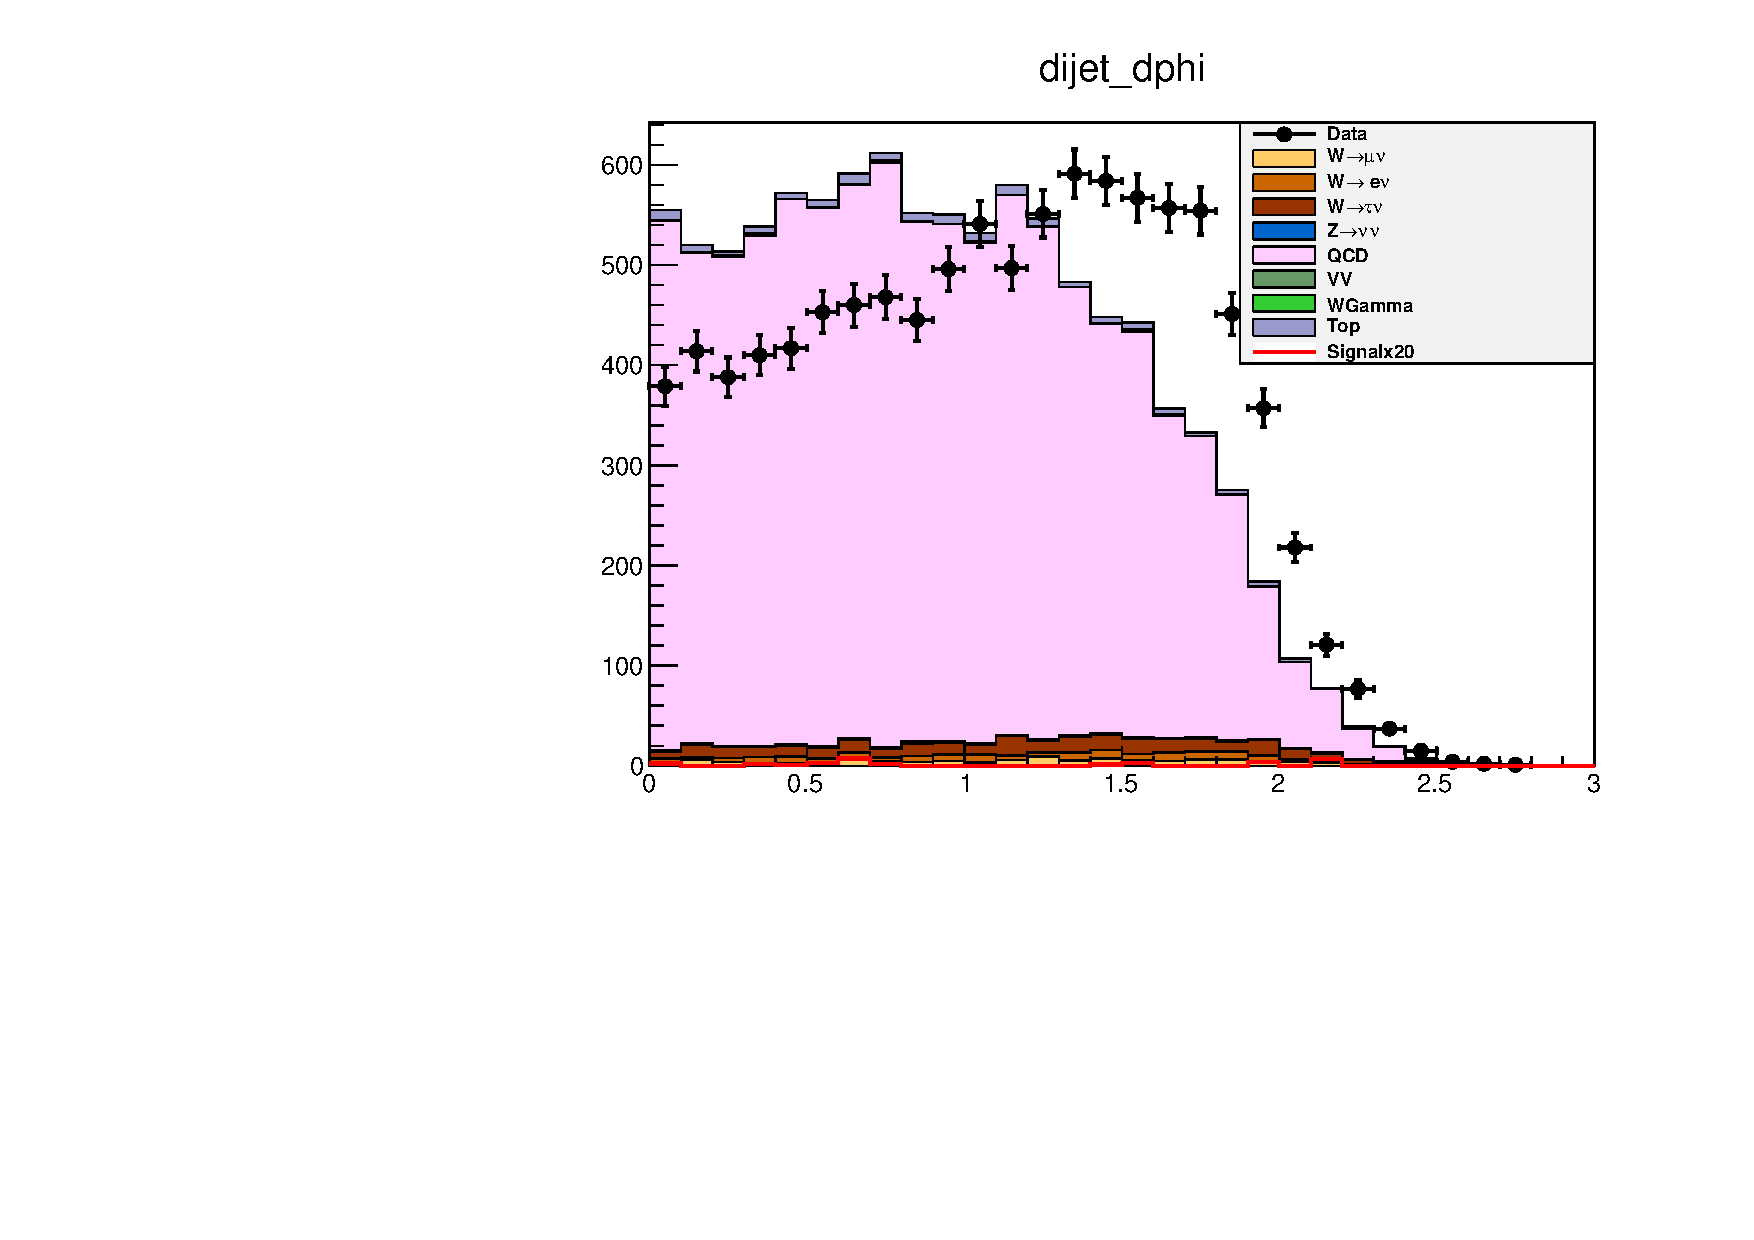
\includegraphics[width=\textwidth]{TalkPics/trigeffprog120814/qcd_dphijj.pdf}
    \end{block}
    \column{.5\textwidth}
    \begin{block}{Jet-MET mindphi}
      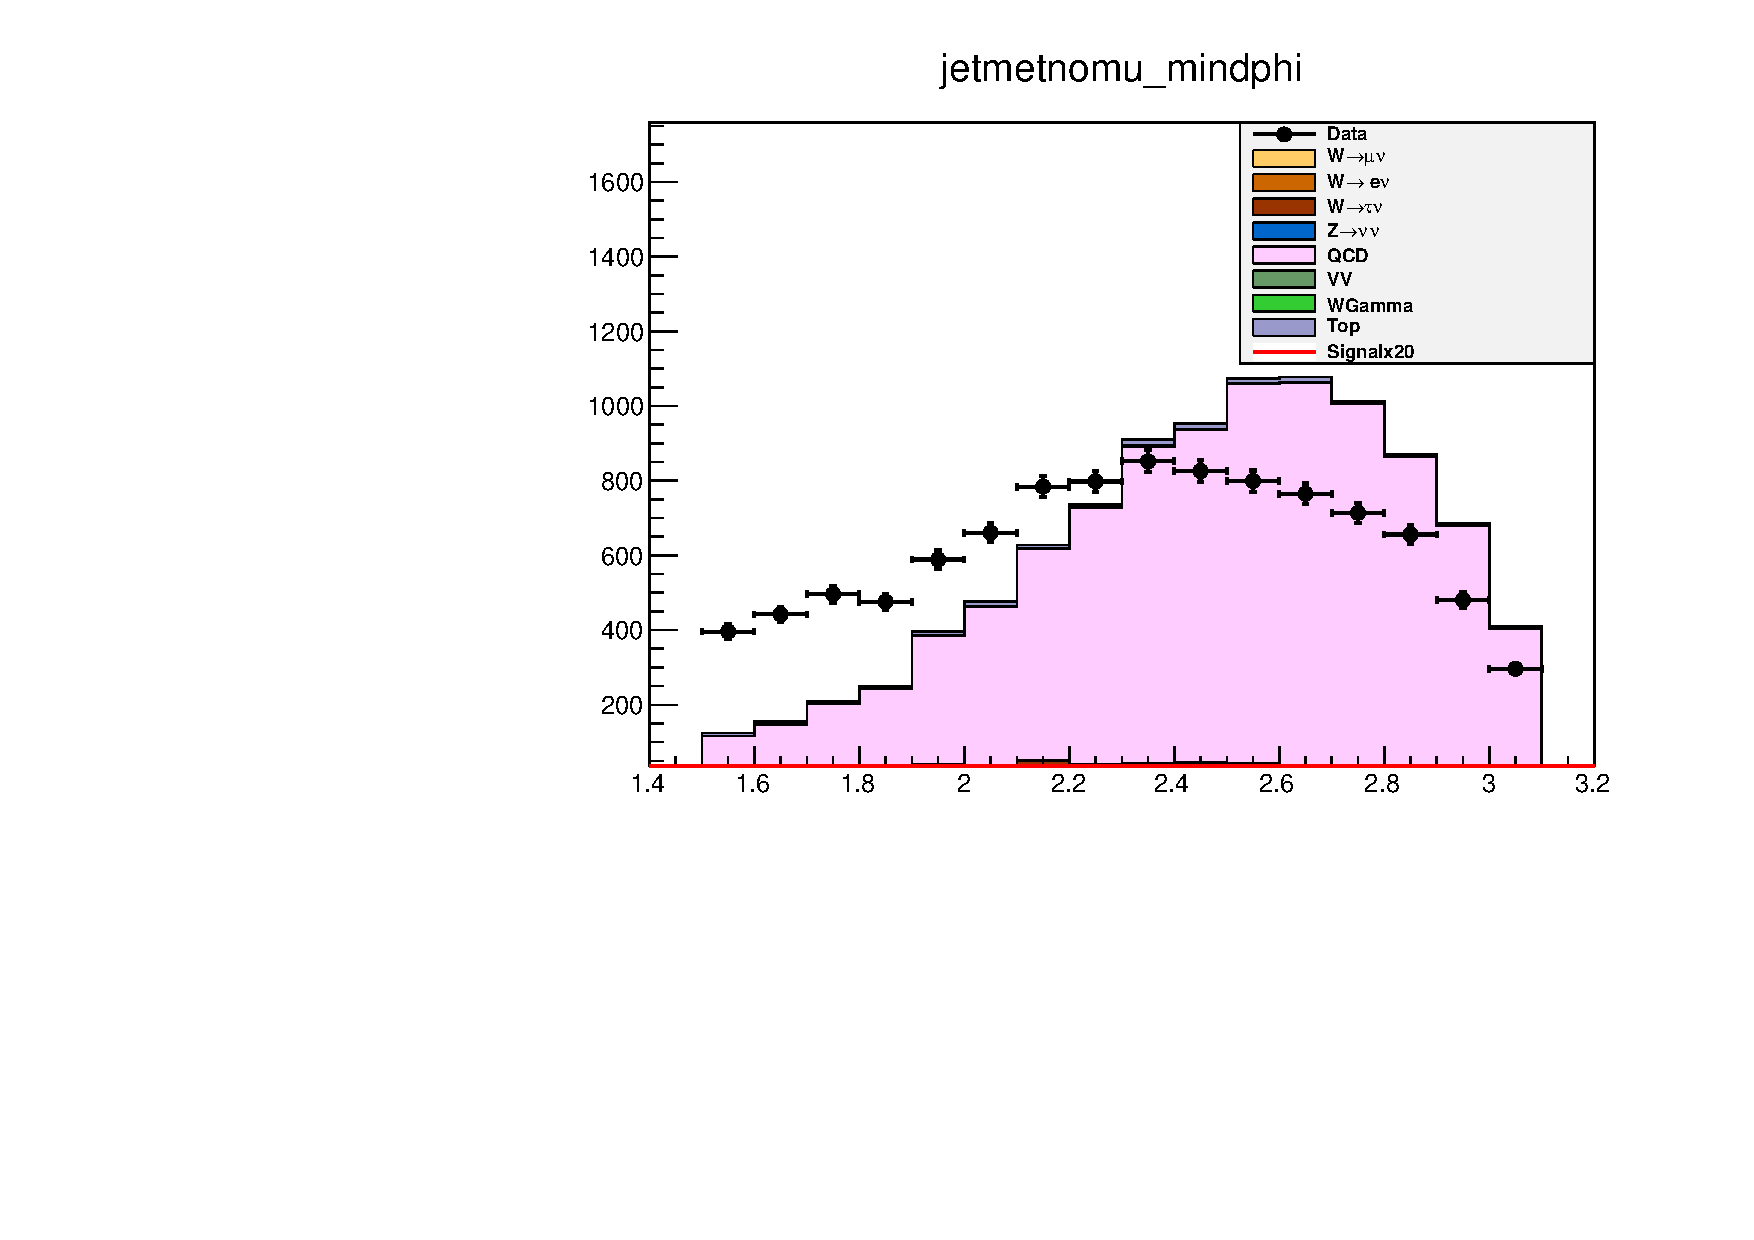
\includegraphics[width=\textwidth]{TalkPics/trigeffprog120814/qcd_jetmetmindphi.pdf}
    \end{block}

  \end{columns}
\end{frame}

\begin{frame}
  \frametitle{New control plots - tight region}
  \begin{columns}
    \column{.5\textwidth}
    \begin{block}{Jet 1 pt}
      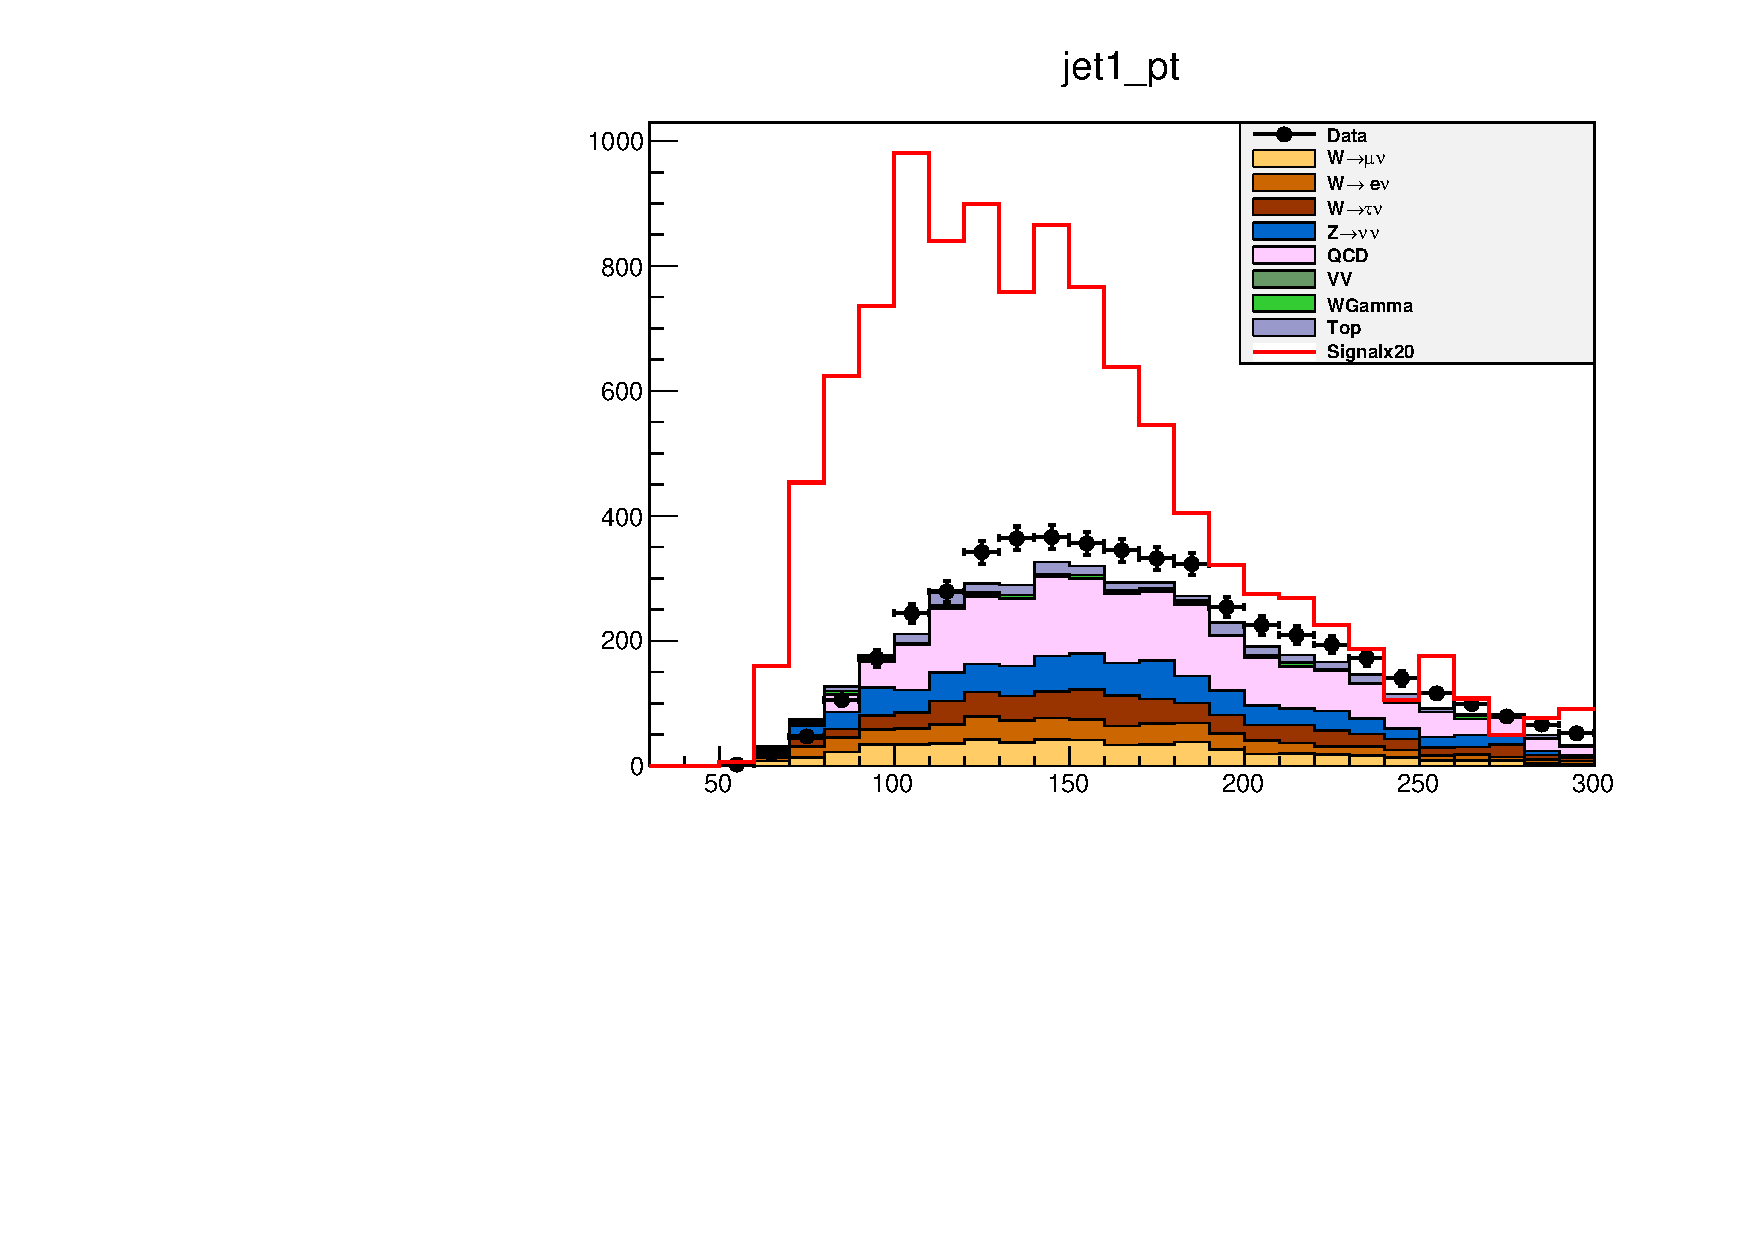
\includegraphics[width=\textwidth]{TalkPics/trigeffprog120814/metandmjjcutsig_jet1pt.pdf}
    \end{block}
    \column{.5\textwidth}
    \begin{block}{Jet 2 pt}
      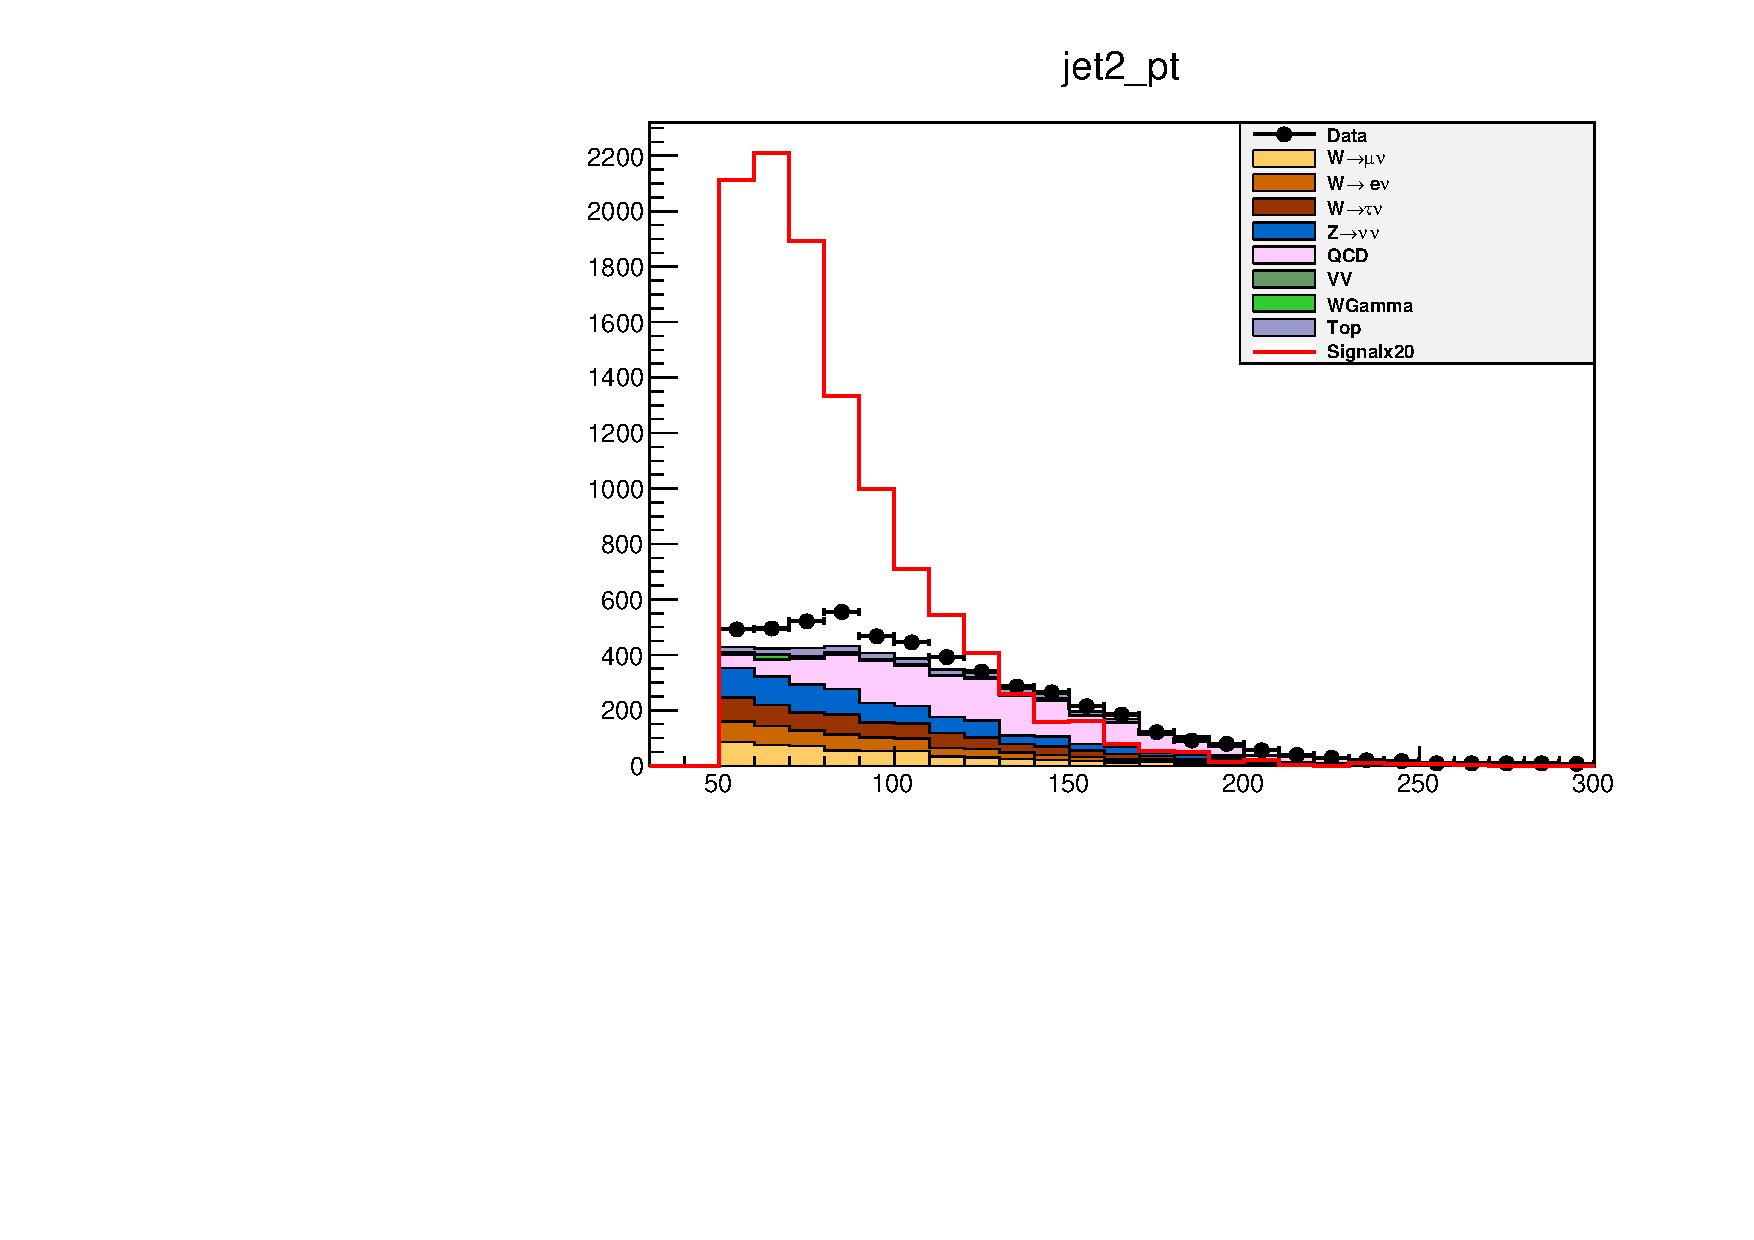
\includegraphics[width=\textwidth]{TalkPics/trigeffprog120814/metandmjjcutsig_jet2pt.pdf}
    \end{block}

  \end{columns}
\end{frame}

\begin{frame}
  \frametitle{New control plots - tight region}
  \begin{columns}
    \column{.5\textwidth}
    \begin{block}{METnomu}
      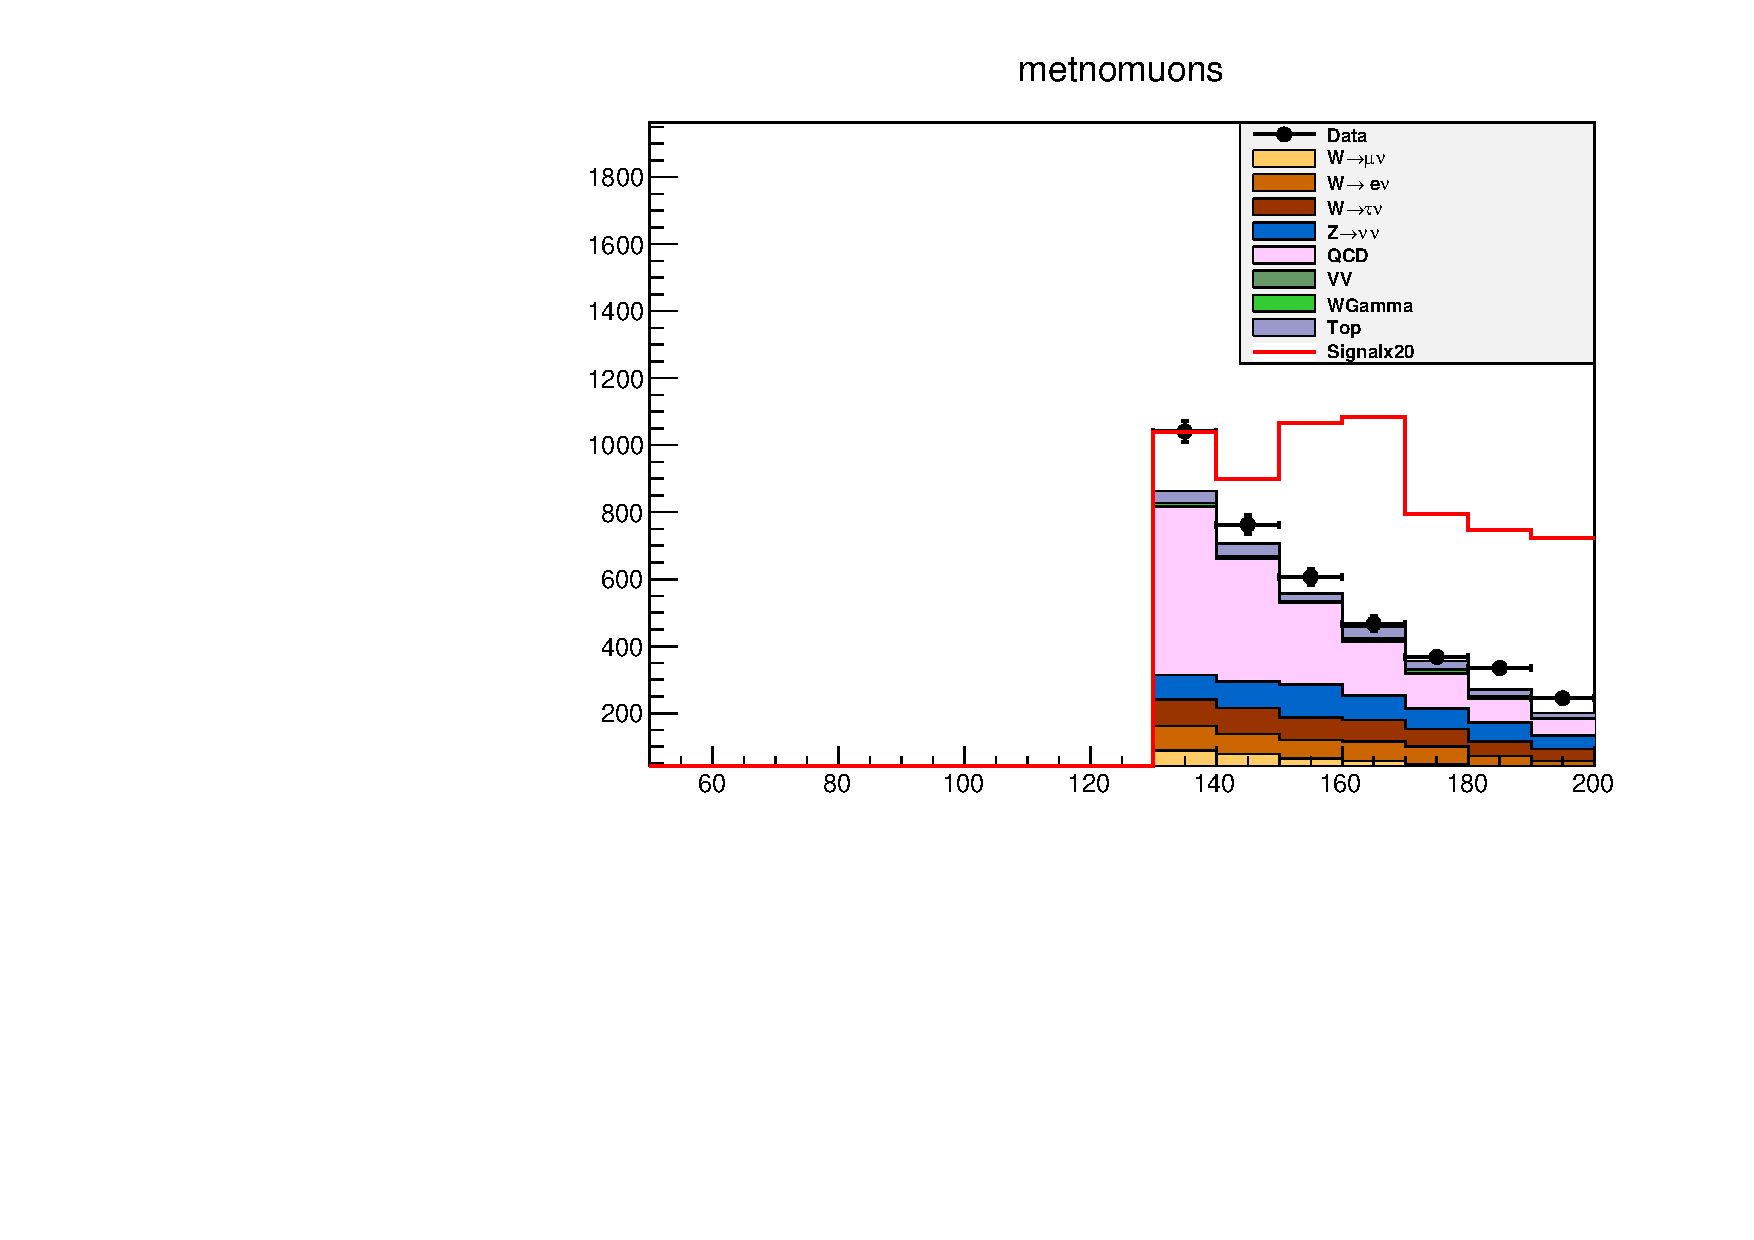
\includegraphics[width=\textwidth]{TalkPics/trigeffprog120814/metandmjjcutsig_metnomu.pdf}
    \end{block}
    \column{.5\textwidth}
    \begin{block}{METnomusig}
      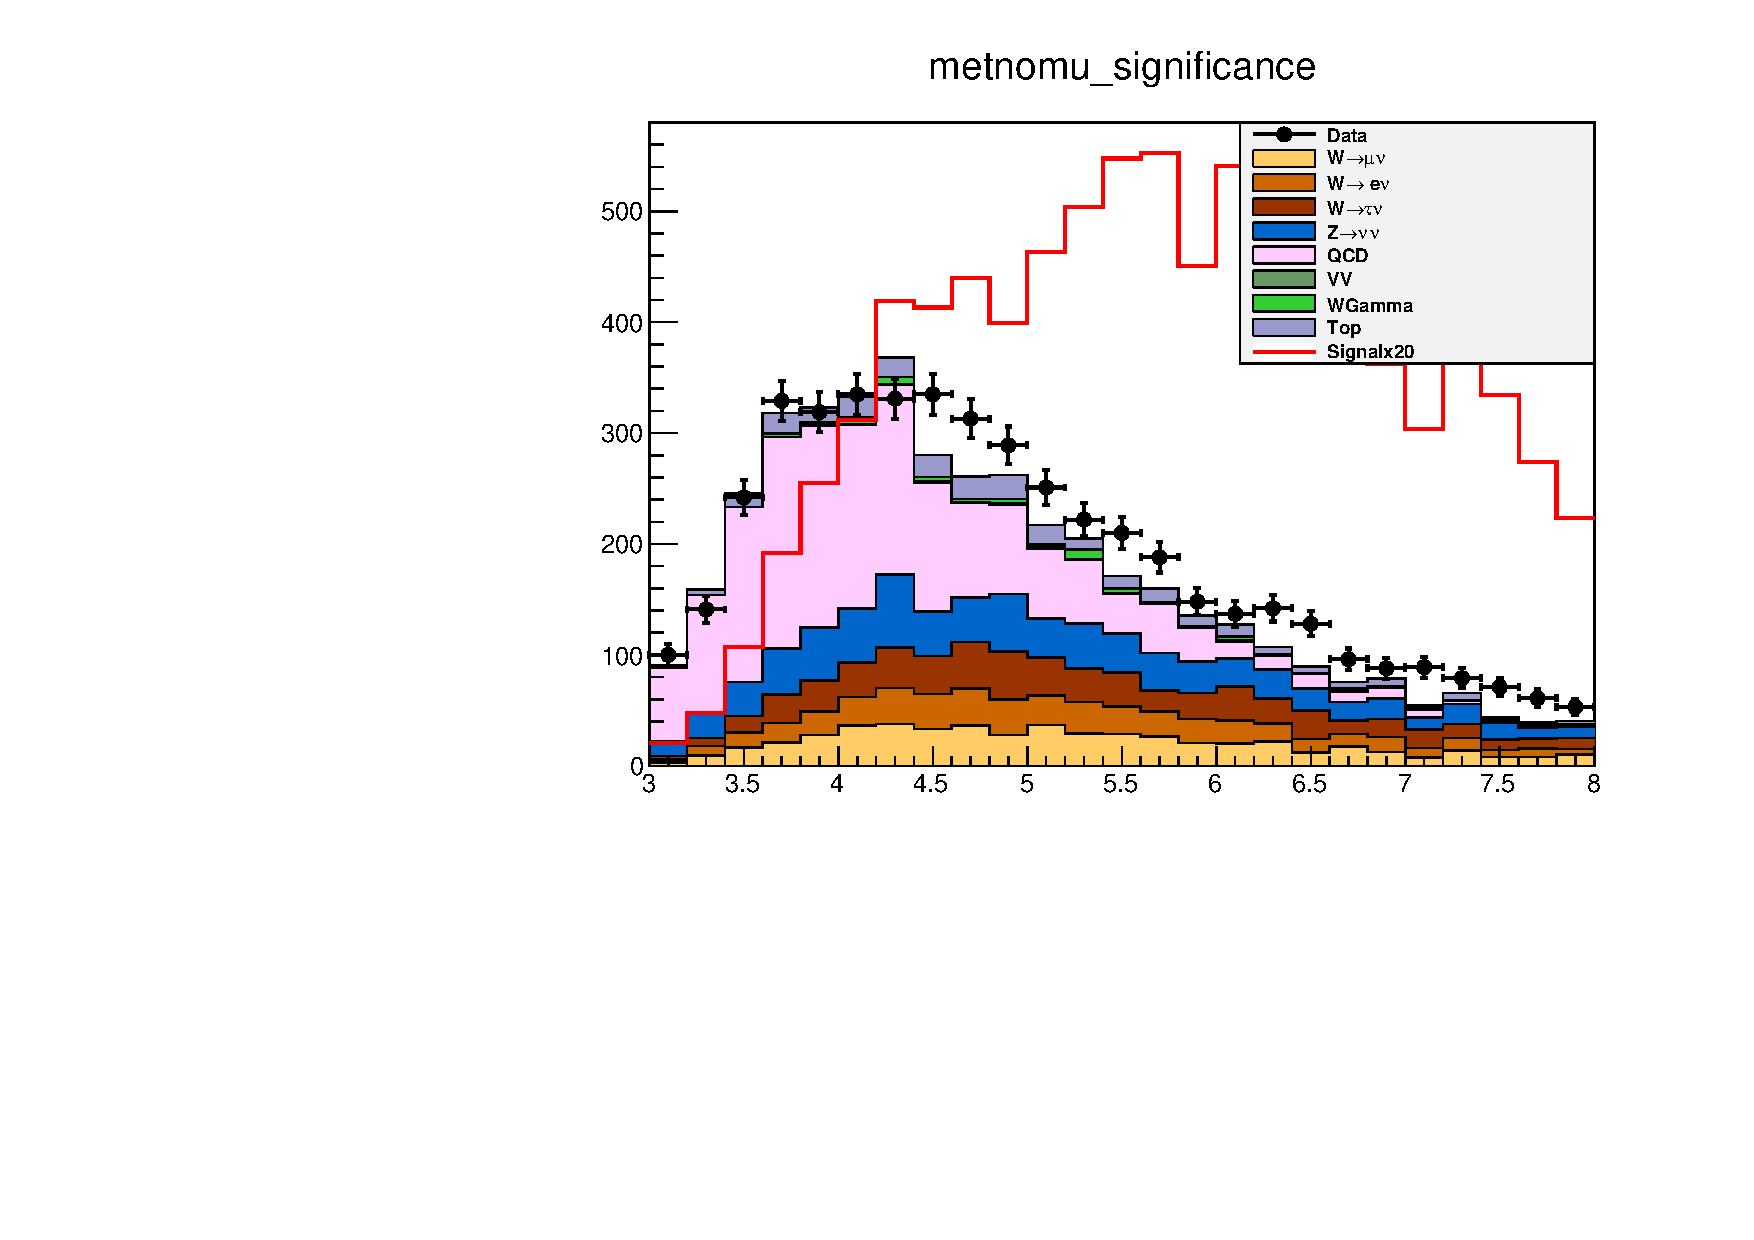
\includegraphics[width=\textwidth]{TalkPics/trigeffprog120814/metandmjjcutsig_metnomusig.pdf}
    \end{block}

  \end{columns}
\end{frame}

\begin{frame}
  \frametitle{New control plots - tight region}
  \begin{columns}
    \column{.5\textwidth}
    \begin{block}{Mjj}
      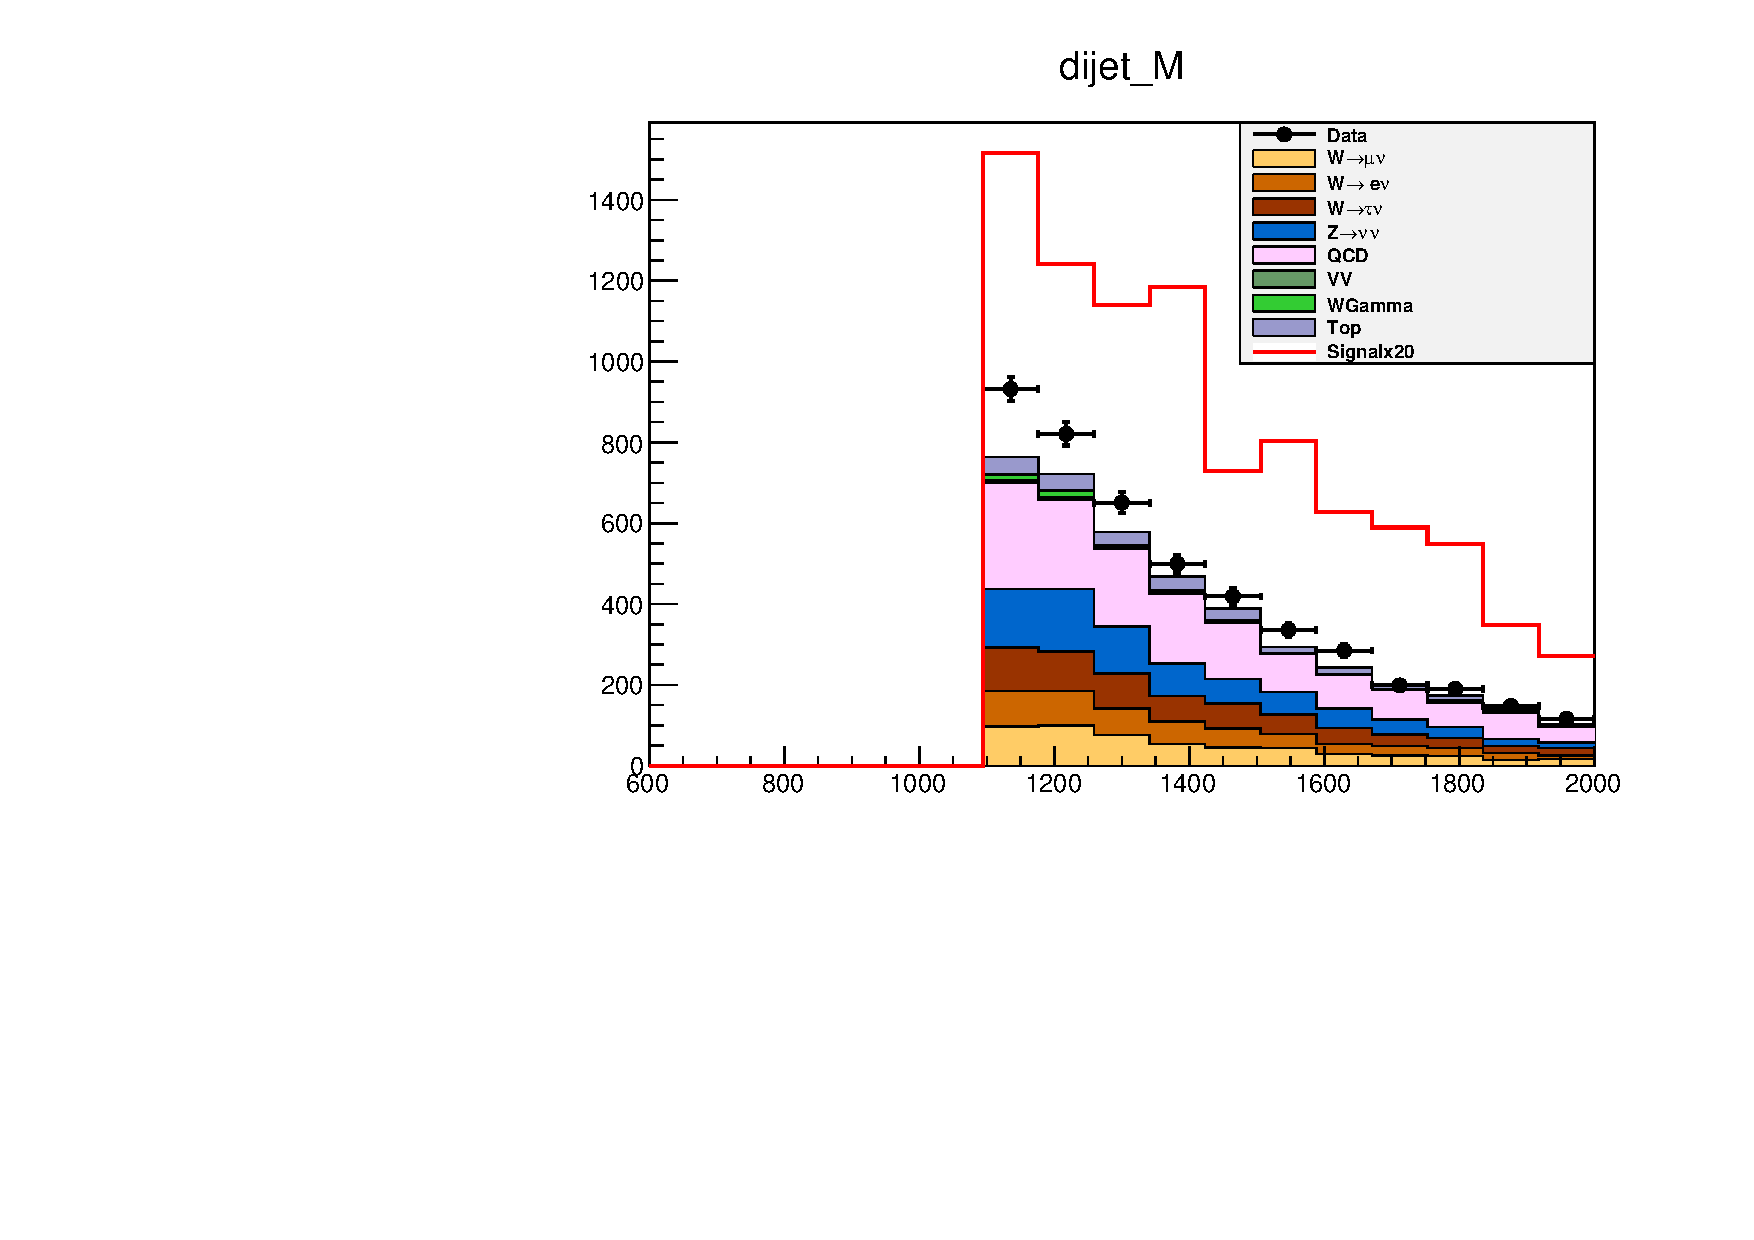
\includegraphics[width=\textwidth]{TalkPics/trigeffprog120814/metandmjjcutsig_mjj.pdf}
    \end{block}
    \column{.5\textwidth}
  \end{columns}
\end{frame}

\begin{frame}
  \frametitle{New control plots - tight region}
  \begin{columns}
    \column{.5\textwidth}
    \begin{block}{Dphijj}
      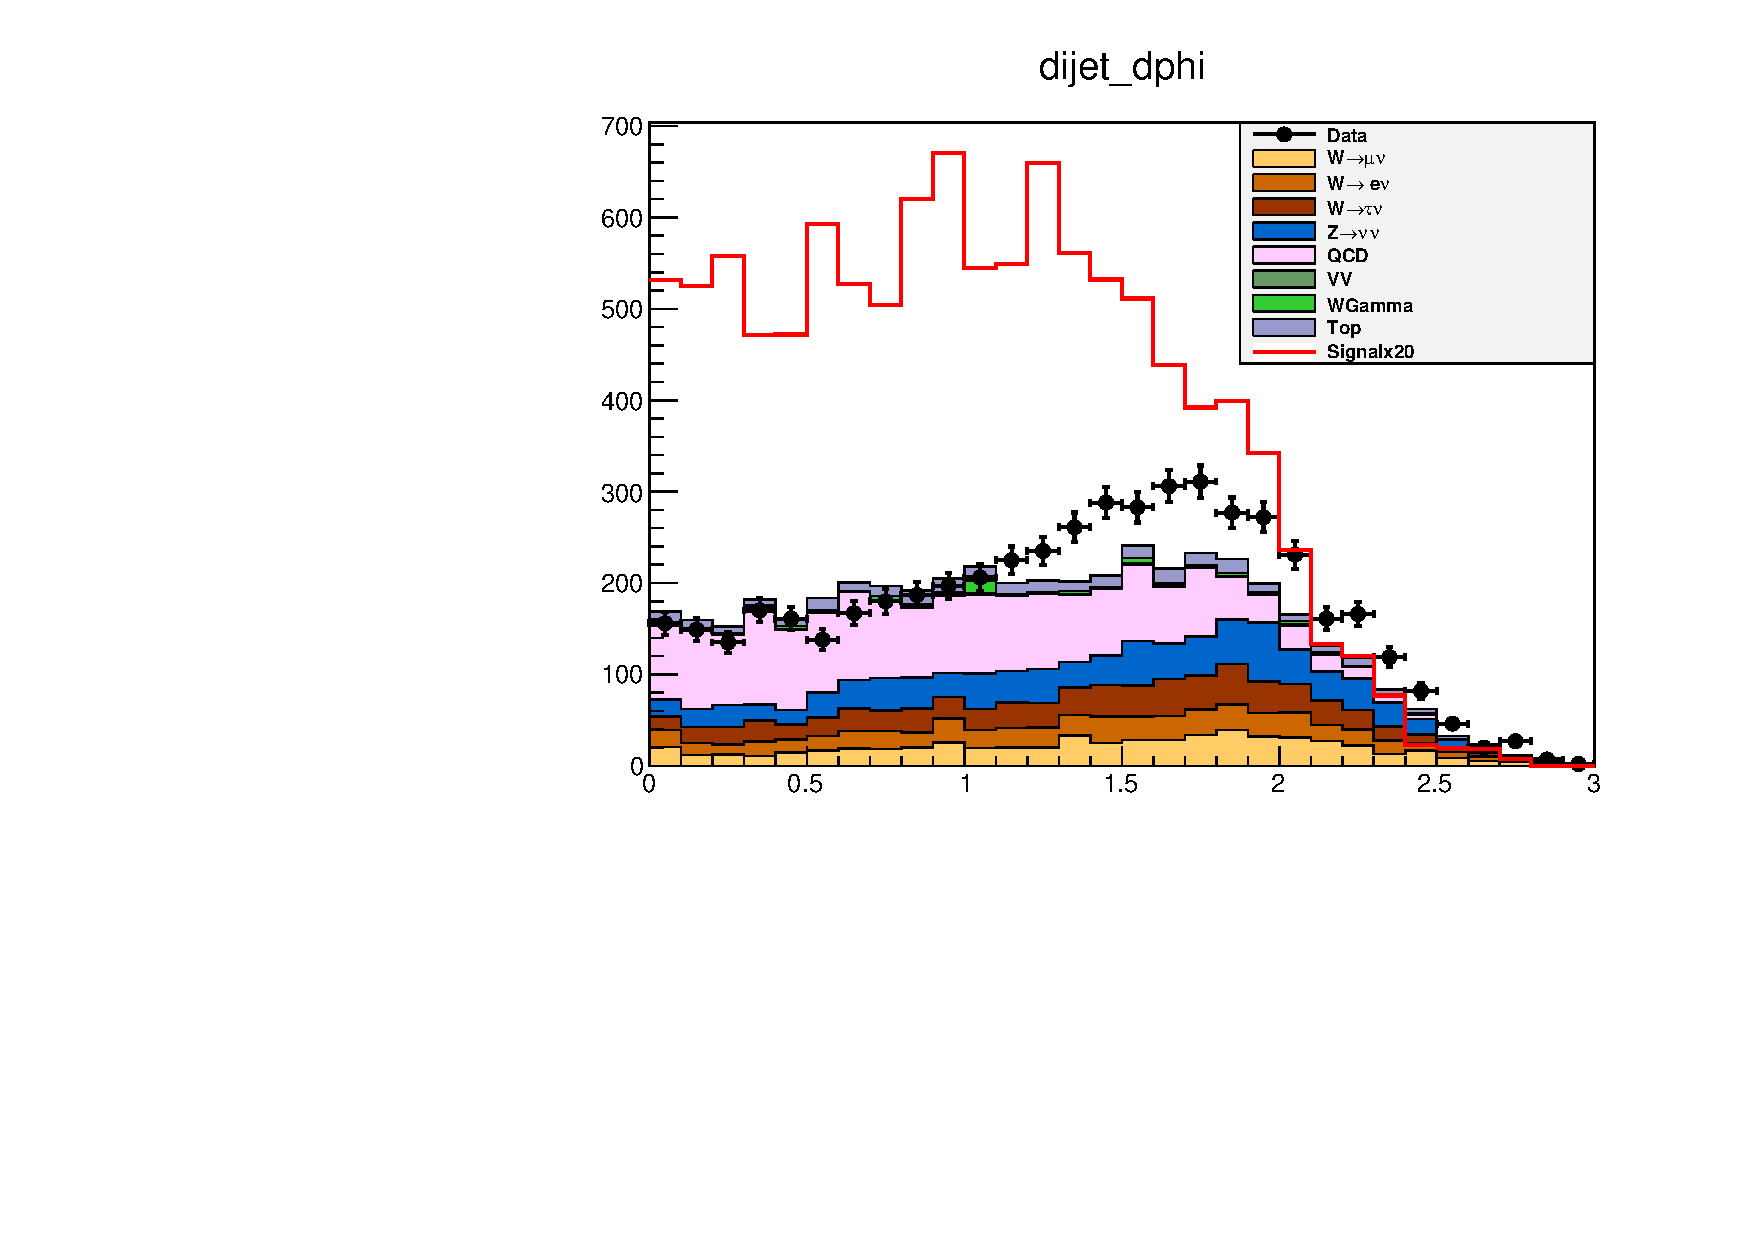
\includegraphics[width=\textwidth]{TalkPics/trigeffprog120814/metandmjjcutsig_dphijj.pdf}
    \end{block}
    \column{.5\textwidth}
    \begin{block}{Detajj}
      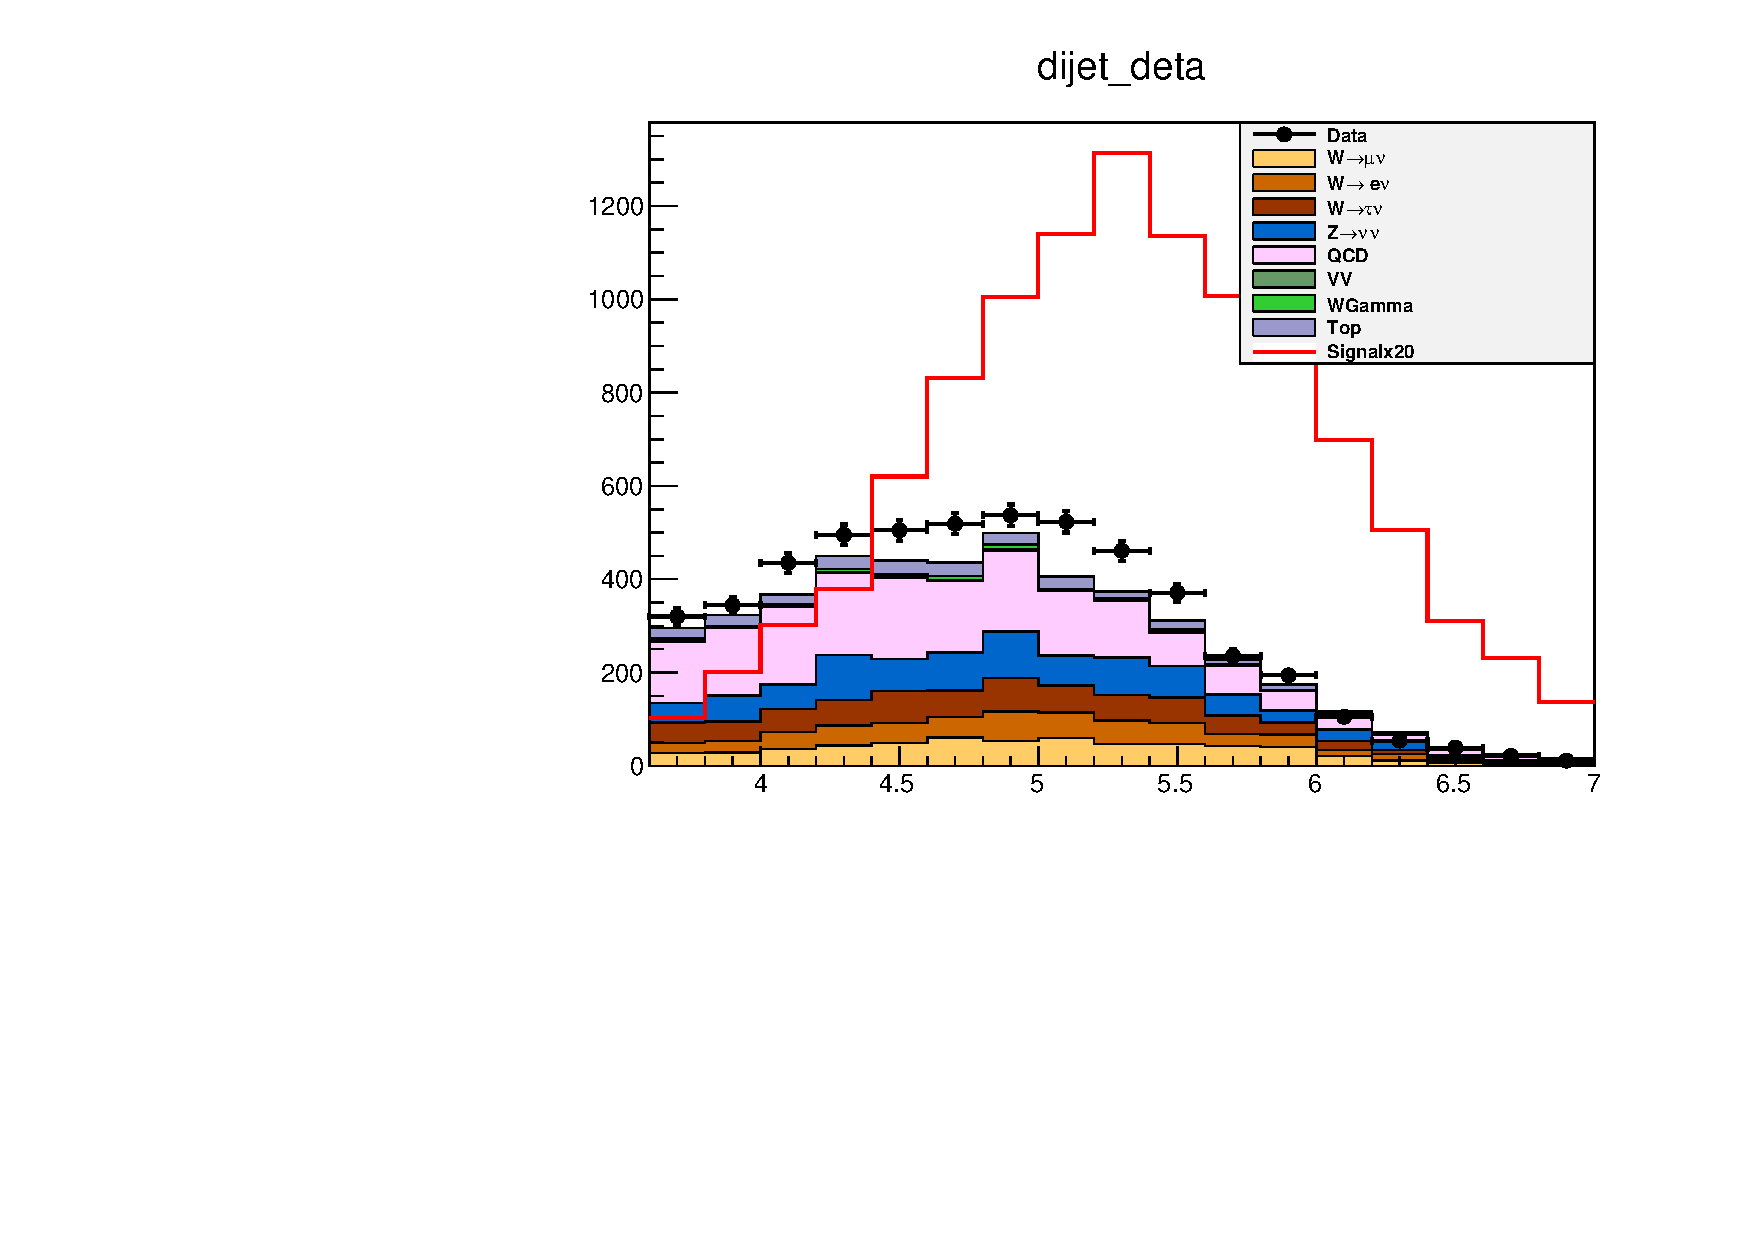
\includegraphics[width=\textwidth]{TalkPics/trigeffprog120814/metandmjjcutsig_detajj.pdf}
    \end{block}

  \end{columns}
\end{frame}

\begin{frame}
  \frametitle{New control plots - tight region}
  \begin{columns}
    \column{.5\textwidth}
    \begin{block}{Jet-met mindphi}
      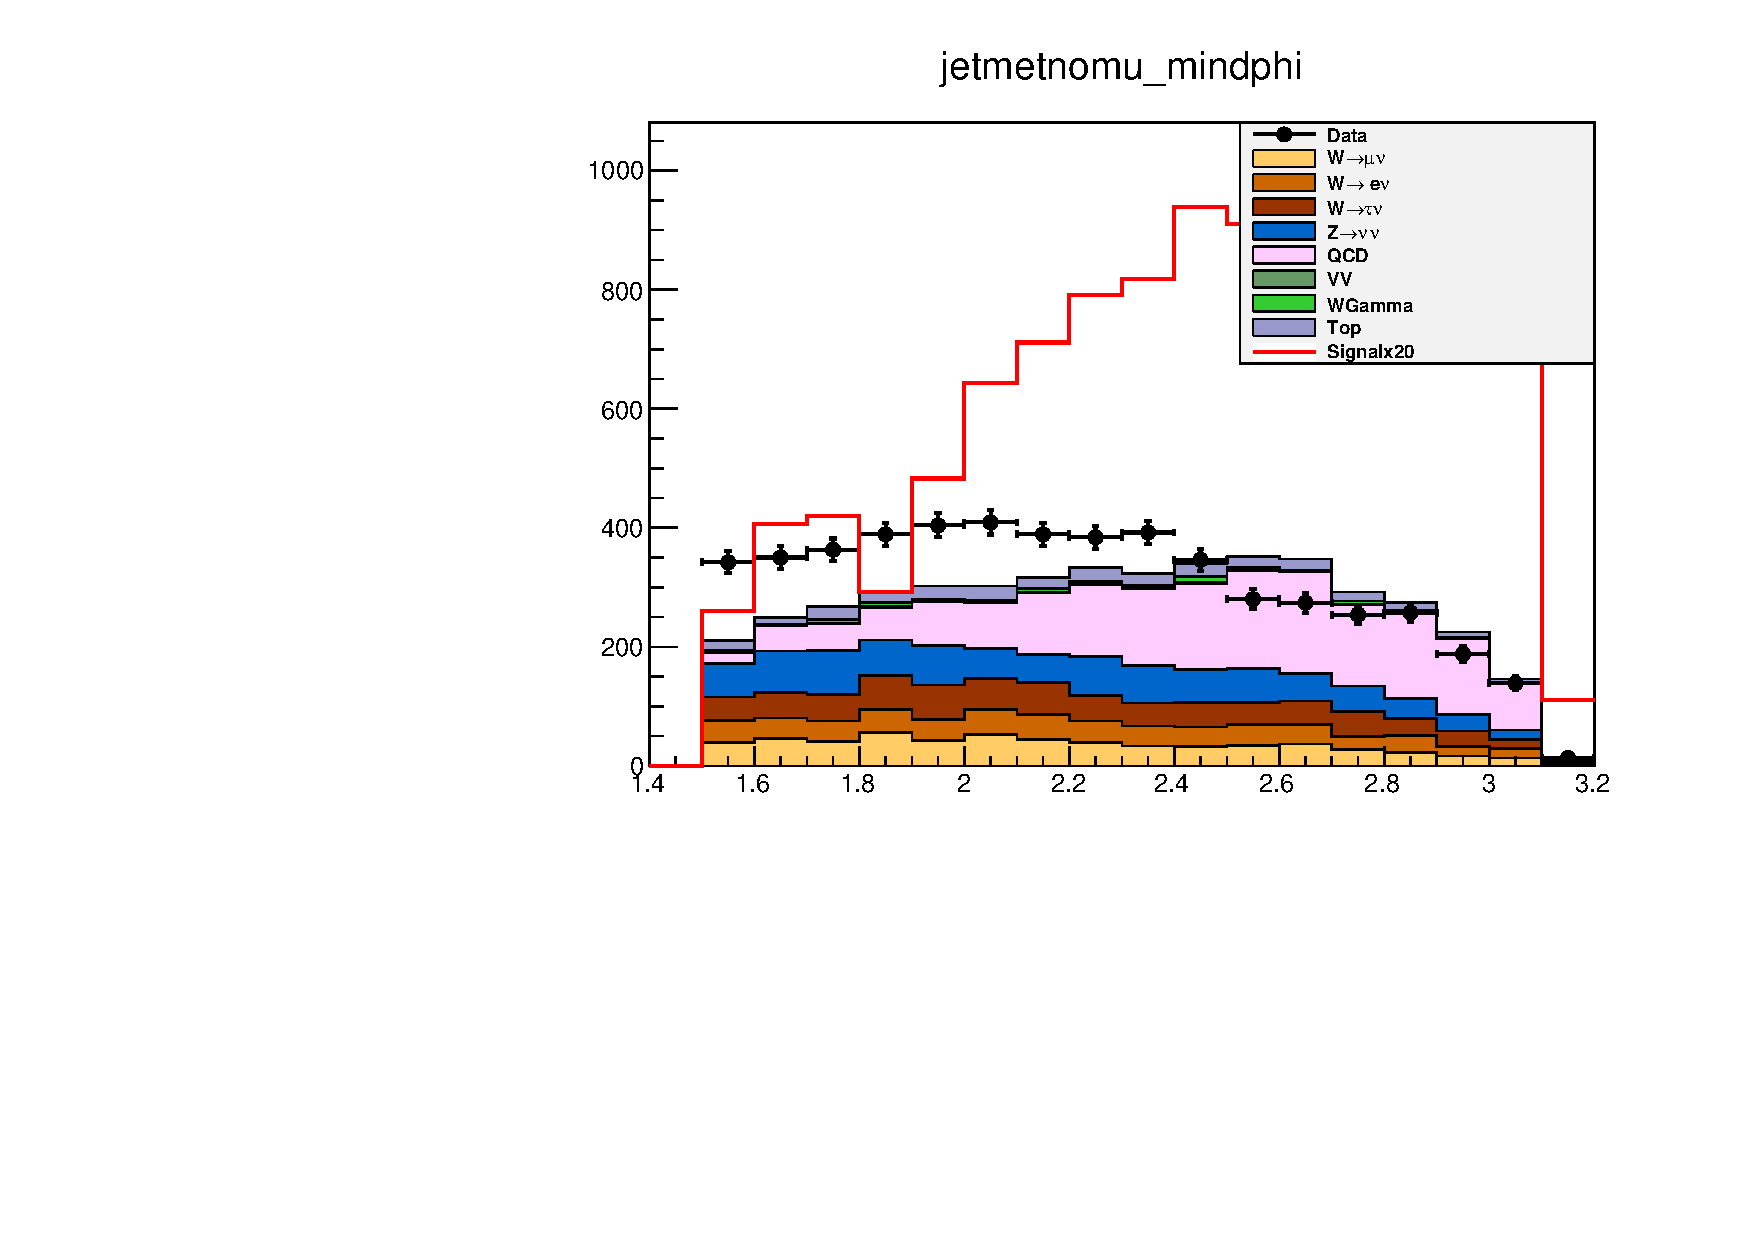
\includegraphics[width=\textwidth]{TalkPics/trigeffprog120814/metandmjjcutsig_jetmetmindphi.pdf}
    \end{block}
    \column{.5\textwidth}
    \begin{block}{dijet-metnomu pt fraction}
      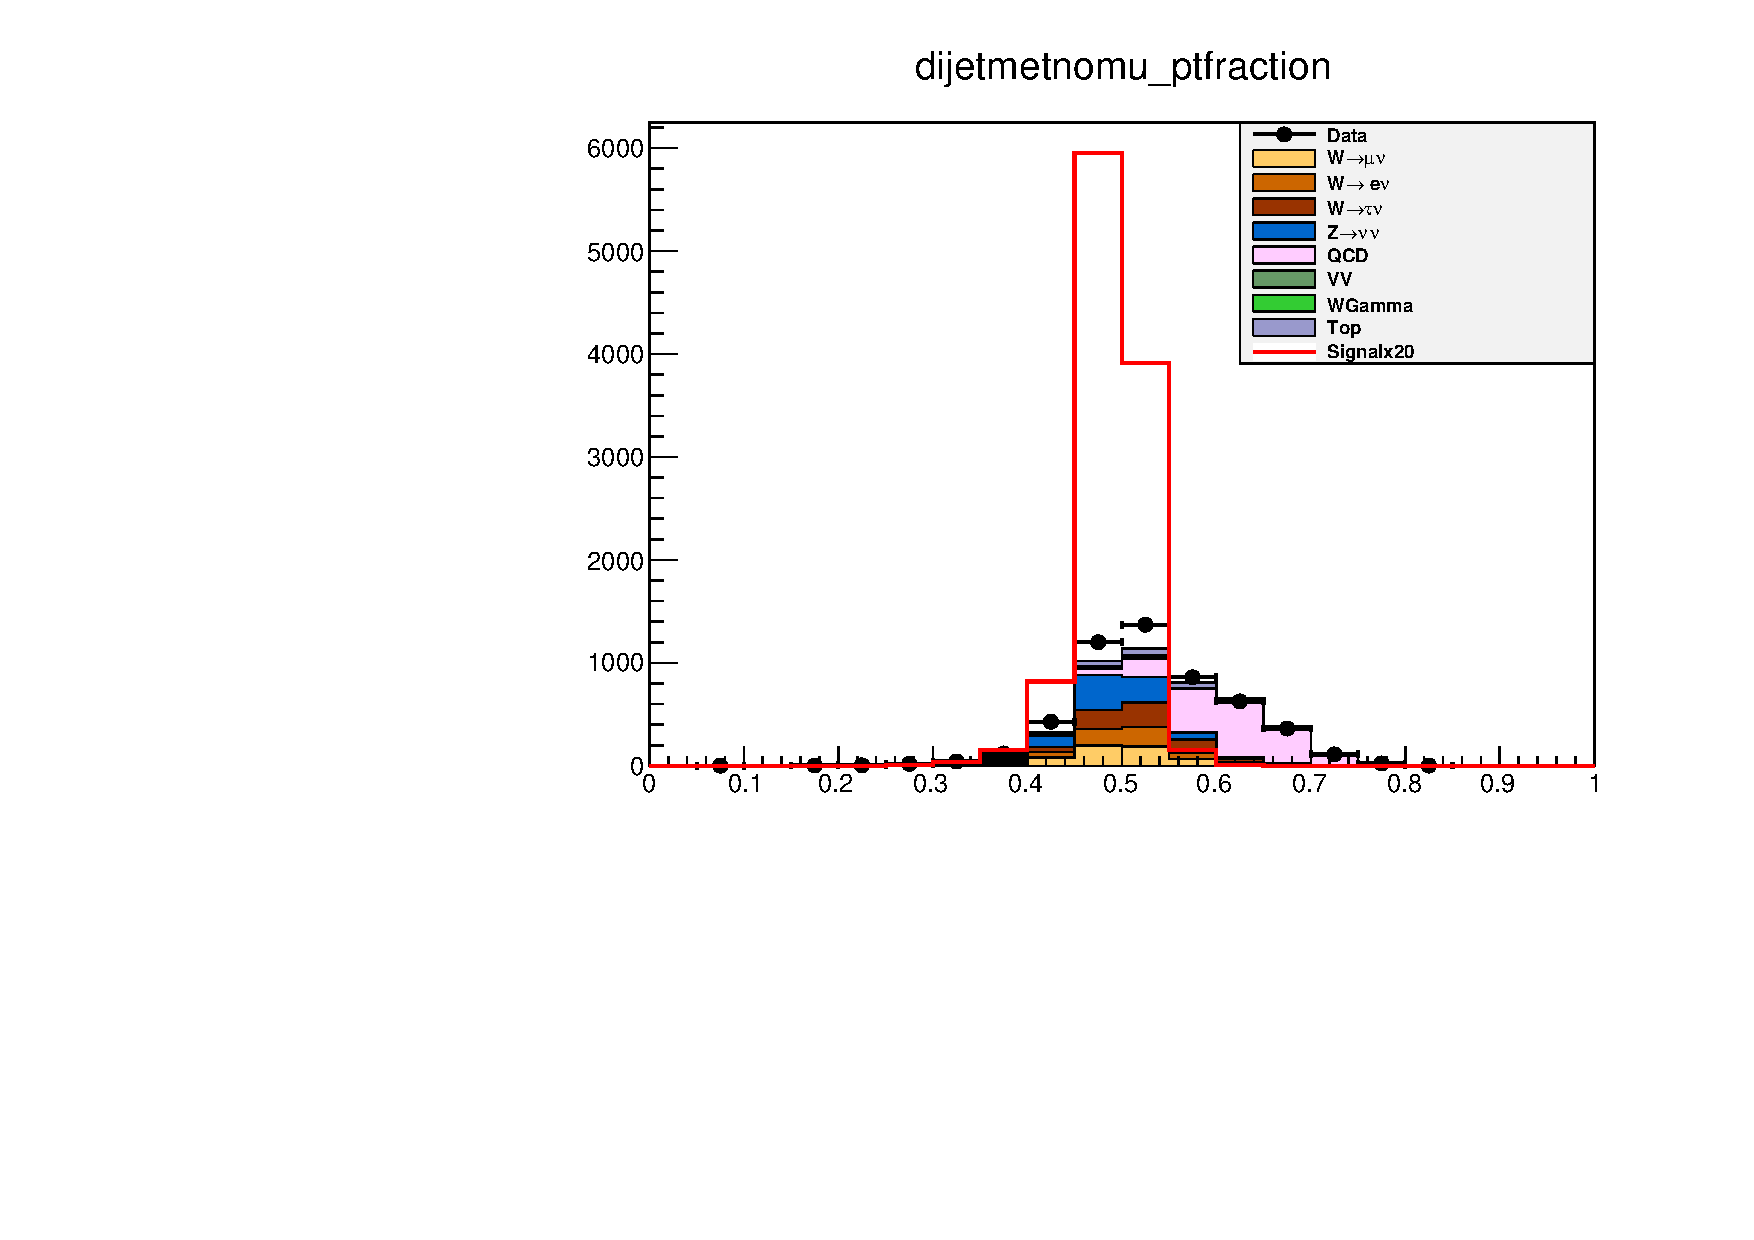
\includegraphics[width=\textwidth]{TalkPics/trigeffprog120814/metandmjjcutsig_dijetmetnomuptfrac.pdf}
    \end{block}

  \end{columns}
\end{frame}


\begin{frame}
  \frametitle{Conclusions}
  \label{lastframe}

  \begin{block}{}
    \scriptsize
    \begin{itemize}
      \item Data MC disagreement still present
      \item[-] Jumps gone due to fitting
      \item[-] Problem with QCD angular distributions
      \item[-] Moving to tight region doesn't remove problem
      \item[-] Have plots only cutting out regions where more than one variable is inefficient, need to study
    \end{itemize}
  \end{block}

\end{frame}

\begin{frame}
  \frametitle{Backup}
\end{frame}

\end{fmffile}
\end{document}
